\documentclass[]{article}
\usepackage{lmodern}
\usepackage{amssymb,amsmath}
\usepackage{ifxetex,ifluatex}
\usepackage{fixltx2e} % provides \textsubscript
\ifnum 0\ifxetex 1\fi\ifluatex 1\fi=0 % if pdftex
  \usepackage[T1]{fontenc}
  \usepackage[utf8]{inputenc}
\else % if luatex or xelatex
  \ifxetex
    \usepackage{mathspec}
  \else
    \usepackage{fontspec}
  \fi
  \defaultfontfeatures{Ligatures=TeX,Scale=MatchLowercase}
\fi
% use upquote if available, for straight quotes in verbatim environments
\IfFileExists{upquote.sty}{\usepackage{upquote}}{}
% use microtype if available
\IfFileExists{microtype.sty}{%
\usepackage{microtype}
\UseMicrotypeSet[protrusion]{basicmath} % disable protrusion for tt fonts
}{}
\usepackage[margin=1in]{geometry}
\usepackage{hyperref}
\hypersetup{unicode=true,
            pdftitle={Comparative evaluation of Differential Gene Expression Analyses Tools},
            pdfauthor={Abdul-Rahman Adamu Bukari},
            pdfborder={0 0 0},
            breaklinks=true}
\urlstyle{same}  % don't use monospace font for urls
\usepackage{color}
\usepackage{fancyvrb}
\newcommand{\VerbBar}{|}
\newcommand{\VERB}{\Verb[commandchars=\\\{\}]}
\DefineVerbatimEnvironment{Highlighting}{Verbatim}{commandchars=\\\{\}}
% Add ',fontsize=\small' for more characters per line
\usepackage{framed}
\definecolor{shadecolor}{RGB}{248,248,248}
\newenvironment{Shaded}{\begin{snugshade}}{\end{snugshade}}
\newcommand{\AlertTok}[1]{\textcolor[rgb]{0.94,0.16,0.16}{#1}}
\newcommand{\AnnotationTok}[1]{\textcolor[rgb]{0.56,0.35,0.01}{\textbf{\textit{#1}}}}
\newcommand{\AttributeTok}[1]{\textcolor[rgb]{0.77,0.63,0.00}{#1}}
\newcommand{\BaseNTok}[1]{\textcolor[rgb]{0.00,0.00,0.81}{#1}}
\newcommand{\BuiltInTok}[1]{#1}
\newcommand{\CharTok}[1]{\textcolor[rgb]{0.31,0.60,0.02}{#1}}
\newcommand{\CommentTok}[1]{\textcolor[rgb]{0.56,0.35,0.01}{\textit{#1}}}
\newcommand{\CommentVarTok}[1]{\textcolor[rgb]{0.56,0.35,0.01}{\textbf{\textit{#1}}}}
\newcommand{\ConstantTok}[1]{\textcolor[rgb]{0.00,0.00,0.00}{#1}}
\newcommand{\ControlFlowTok}[1]{\textcolor[rgb]{0.13,0.29,0.53}{\textbf{#1}}}
\newcommand{\DataTypeTok}[1]{\textcolor[rgb]{0.13,0.29,0.53}{#1}}
\newcommand{\DecValTok}[1]{\textcolor[rgb]{0.00,0.00,0.81}{#1}}
\newcommand{\DocumentationTok}[1]{\textcolor[rgb]{0.56,0.35,0.01}{\textbf{\textit{#1}}}}
\newcommand{\ErrorTok}[1]{\textcolor[rgb]{0.64,0.00,0.00}{\textbf{#1}}}
\newcommand{\ExtensionTok}[1]{#1}
\newcommand{\FloatTok}[1]{\textcolor[rgb]{0.00,0.00,0.81}{#1}}
\newcommand{\FunctionTok}[1]{\textcolor[rgb]{0.00,0.00,0.00}{#1}}
\newcommand{\ImportTok}[1]{#1}
\newcommand{\InformationTok}[1]{\textcolor[rgb]{0.56,0.35,0.01}{\textbf{\textit{#1}}}}
\newcommand{\KeywordTok}[1]{\textcolor[rgb]{0.13,0.29,0.53}{\textbf{#1}}}
\newcommand{\NormalTok}[1]{#1}
\newcommand{\OperatorTok}[1]{\textcolor[rgb]{0.81,0.36,0.00}{\textbf{#1}}}
\newcommand{\OtherTok}[1]{\textcolor[rgb]{0.56,0.35,0.01}{#1}}
\newcommand{\PreprocessorTok}[1]{\textcolor[rgb]{0.56,0.35,0.01}{\textit{#1}}}
\newcommand{\RegionMarkerTok}[1]{#1}
\newcommand{\SpecialCharTok}[1]{\textcolor[rgb]{0.00,0.00,0.00}{#1}}
\newcommand{\SpecialStringTok}[1]{\textcolor[rgb]{0.31,0.60,0.02}{#1}}
\newcommand{\StringTok}[1]{\textcolor[rgb]{0.31,0.60,0.02}{#1}}
\newcommand{\VariableTok}[1]{\textcolor[rgb]{0.00,0.00,0.00}{#1}}
\newcommand{\VerbatimStringTok}[1]{\textcolor[rgb]{0.31,0.60,0.02}{#1}}
\newcommand{\WarningTok}[1]{\textcolor[rgb]{0.56,0.35,0.01}{\textbf{\textit{#1}}}}
\usepackage{graphicx}
% grffile has become a legacy package: https://ctan.org/pkg/grffile
\IfFileExists{grffile.sty}{%
\usepackage{grffile}
}{}
\makeatletter
\def\maxwidth{\ifdim\Gin@nat@width>\linewidth\linewidth\else\Gin@nat@width\fi}
\def\maxheight{\ifdim\Gin@nat@height>\textheight\textheight\else\Gin@nat@height\fi}
\makeatother
% Scale images if necessary, so that they will not overflow the page
% margins by default, and it is still possible to overwrite the defaults
% using explicit options in \includegraphics[width, height, ...]{}
\setkeys{Gin}{width=\maxwidth,height=\maxheight,keepaspectratio}
\IfFileExists{parskip.sty}{%
\usepackage{parskip}
}{% else
\setlength{\parindent}{0pt}
\setlength{\parskip}{6pt plus 2pt minus 1pt}
}
\setlength{\emergencystretch}{3em}  % prevent overfull lines
\providecommand{\tightlist}{%
  \setlength{\itemsep}{0pt}\setlength{\parskip}{0pt}}
\setcounter{secnumdepth}{0}
% Redefines (sub)paragraphs to behave more like sections
\ifx\paragraph\undefined\else
\let\oldparagraph\paragraph
\renewcommand{\paragraph}[1]{\oldparagraph{#1}\mbox{}}
\fi
\ifx\subparagraph\undefined\else
\let\oldsubparagraph\subparagraph
\renewcommand{\subparagraph}[1]{\oldsubparagraph{#1}\mbox{}}
\fi

%%% Use protect on footnotes to avoid problems with footnotes in titles
\let\rmarkdownfootnote\footnote%
\def\footnote{\protect\rmarkdownfootnote}

%%% Change title format to be more compact
\usepackage{titling}

% Create subtitle command for use in maketitle
\providecommand{\subtitle}[1]{
  \posttitle{
    \begin{center}\large#1\end{center}
    }
}

\setlength{\droptitle}{-2em}

  \title{Comparative evaluation of Differential Gene Expression Analyses Tools}
    \pretitle{\vspace{\droptitle}\centering\huge}
  \posttitle{\par}
    \author{Abdul-Rahman Adamu Bukari}
    \preauthor{\centering\large\emph}
  \postauthor{\par}
      \predate{\centering\large\emph}
  \postdate{\par}
    \date{11/11/2019}


\begin{document}
\maketitle

\DeclareUnicodeCharacter{2212}{-}

\begin{Shaded}
\begin{Highlighting}[]
\KeywordTok{library}\NormalTok{(}\StringTok{"pheatmap"}\NormalTok{)}
\KeywordTok{library}\NormalTok{(}\StringTok{"tibble"}\NormalTok{)}
\KeywordTok{library}\NormalTok{(}\StringTok{"compcodeR"}\NormalTok{)}
\KeywordTok{library}\NormalTok{(}\StringTok{"here"}\NormalTok{)}
\KeywordTok{library}\NormalTok{(}\StringTok{"ggplot2"}\NormalTok{)}
\KeywordTok{library}\NormalTok{(}\StringTok{"RColorBrewer"}\NormalTok{)}
\KeywordTok{library}\NormalTok{(}\StringTok{"affy"}\NormalTok{)}
\KeywordTok{library}\NormalTok{(}\StringTok{"readr"}\NormalTok{)}
\KeywordTok{library}\NormalTok{(}\StringTok{"DESeq2"}\NormalTok{)}
\KeywordTok{library}\NormalTok{(}\StringTok{"apeglm"}\NormalTok{)}
\KeywordTok{library}\NormalTok{(}\StringTok{"NOISeq"}\NormalTok{)}
\KeywordTok{library}\NormalTok{(}\StringTok{"DEGseq"}\NormalTok{)}
\end{Highlighting}
\end{Shaded}

\hypertarget{introduction}{%
\subsection{Introduction}\label{introduction}}

A crucial component of RNA sequence analysis is the statistical
procedure used to call differentially expressed genes. Yet existing
methods for differential gene expression analysis presume that count
data follows specific distribution models (Huang, Niu, and Qin (2015)).
These baseline assumptions along with other downstream assumptions
result in a list of differentially expressed genes with potentially
differing accuracies which could affect downstream analysis such as
functional enrichment analysis. Here, using simulated datasets, the
accuracies of three DGE analysis tools (Deseq2, NOISeq, DEGseq)
operating with different models (Negative Binomial, Non-parametric and
Binomial distributions respectively) will be assessed and the
theoretical underpinnings of the differences in the outcomes will be
explained.

\hypertarget{methods}{%
\subsection{Methods}\label{methods}}

\hypertarget{choice-of-data-simulation-tool}{%
\subsubsection{Choice of data simulation
tool}\label{choice-of-data-simulation-tool}}

There are at least 4 tools developed specifically for simulating RNAseq
count data. Interestingly, all the tools simulate count data following a
Negative-Binomial distribution. This is due to the over-dispertion
recognized in real expression datasets. Thus the variance of the
expression values is larger than the mean values. This is a better
alternative to the poison distributin which assumes no difference
beteeen the mean and variance.

\href{https://rdrr.io/bioc/PROPER/man/simRNAseq.html}{\emph{simRNAseq}}
from PROPER

\href{chrome-extension://cbnaodkpfinfiipjblikofhlhlcickei/src/pdfviewer/web/viewer.html?file=https://cran.r-project.org/web/packages/ssizeRNA/ssizeRNA.pdf}{\emph{sim.counts}}
from ssizeRNA

\href{https://bioconductor.org/packages/release/bioc/manuals/compcodeR/man/compcodeR.pdf}{\emph{generateSyntheticData}}
from compcodeR

\href{https://www.rdocumentation.org/packages/metaseqR/versions/1.12.2/topics/make.sim.data.sd}{\emph{make.sim.data.sd}}
from metaseqR

The functions \emph{generateSyntheticData} and \emph{make.sim.data.sd}
both work by generating synthetic RNA-seq count matrices, using the
approaches described by Robles et al. (2012) and Soneson and Delorenzi
(2013). The \emph{generateSyntheticData} function was used in simulating
the synthetic data due to the extensive documentation that support the
development of this function. Additionally, unlike
\emph{make.sim.data.sd} which samples from one real data, mean values
can be sampled from values estimated from the both the Pickrell and
Cheung datasets.

\hypertarget{data-simulation}{%
\subsubsection{Data simulation}\label{data-simulation}}

Four simulated datasets (D1, D2, D3, D4) were generated using the same
parameters to asses the consistency of the differential expression
analysis tools. The simulated datasets contained 13000 gene counts with
two groups (group1 and group2) of 5 replicates each, where 1300 of the
genes were simulated to be differentially expressed between the two
groups. The counts were also simulated with the same dispersion in the
two groups, and no outlier counts were introduced. The datasets were
then filtered by excluding all genes with total counts of 0. The
differentially expressed genes were equally distributed between
upregulated and downregulated genes.The \emph{summarizeSynthetic} was
then used to generate a report summarizing the parameters that were used
for the simulation in addition to some diagnostic plots.

\begin{Shaded}
\begin{Highlighting}[]
\CommentTok{#Run the simulation code}
\NormalTok{D1 <-}\StringTok{ }\KeywordTok{generateSyntheticData}\NormalTok{(}\DataTypeTok{dataset =} \StringTok{"D1"}\NormalTok{, }\DataTypeTok{n.vars =} \DecValTok{13000}\NormalTok{,}
             \DataTypeTok{samples.per.cond =} \DecValTok{5}\NormalTok{, }\DataTypeTok{n.diffexp =} \DecValTok{1300}\NormalTok{,}\DataTypeTok{repl.id =} \DecValTok{1}\NormalTok{, }\DataTypeTok{seqdepth =} \FloatTok{1e8}\NormalTok{,}
             \DataTypeTok{fraction.upregulated =} \FloatTok{0.5}\NormalTok{, }\DataTypeTok{between.group.diffdisp =} \OtherTok{FALSE}\NormalTok{,}
             \DataTypeTok{filter.threshold.total =} \DecValTok{1}\NormalTok{,}\DataTypeTok{filter.threshold.mediancpm =} \DecValTok{0}\NormalTok{,}
             \DataTypeTok{fraction.non.overdispersed =} \DecValTok{0}\NormalTok{,}\DataTypeTok{output.file =} \StringTok{"D1.rds"}\NormalTok{)}

\CommentTok{#extract the Truth set}
\NormalTok{D1_truthset <-}\StringTok{ }\KeywordTok{subset}\NormalTok{(D1}\OperatorTok{@}\NormalTok{variable.annotations, differential.expression }\OperatorTok{==}\DecValTok{1}\NormalTok{)}
\KeywordTok{nrow}\NormalTok{(D1_truthset)}
\end{Highlighting}
\end{Shaded}

\begin{verbatim}
## [1] 1300
\end{verbatim}

\begin{Shaded}
\begin{Highlighting}[]
\KeywordTok{write.csv}\NormalTok{(D1_truthset,}\StringTok{'D1_truthset.csv'}\NormalTok{)}
\end{Highlighting}
\end{Shaded}

\begin{Shaded}
\begin{Highlighting}[]
\NormalTok{D2 <-}\StringTok{ }\KeywordTok{generateSyntheticData}\NormalTok{(}\DataTypeTok{dataset =} \StringTok{"D2"}\NormalTok{, }\DataTypeTok{n.vars =} \DecValTok{13000}\NormalTok{,}
             \DataTypeTok{samples.per.cond =} \DecValTok{5}\NormalTok{, }\DataTypeTok{n.diffexp =} \DecValTok{1300}\NormalTok{,}\DataTypeTok{repl.id =} \DecValTok{2}\NormalTok{, }\DataTypeTok{seqdepth =} \FloatTok{1e8}\NormalTok{,}
             \DataTypeTok{fraction.upregulated =} \FloatTok{0.5}\NormalTok{, }\DataTypeTok{between.group.diffdisp =} \OtherTok{FALSE}\NormalTok{,}
             \DataTypeTok{filter.threshold.total =} \DecValTok{1}\NormalTok{,}\DataTypeTok{filter.threshold.mediancpm =} \DecValTok{0}\NormalTok{,}
             \DataTypeTok{fraction.non.overdispersed =} \DecValTok{0}\NormalTok{,}\DataTypeTok{output.file =} \StringTok{"D2.rds"}\NormalTok{)}
\NormalTok{D2_truthset <-}\StringTok{ }\KeywordTok{subset}\NormalTok{(D2}\OperatorTok{@}\NormalTok{variable.annotations, differential.expression }\OperatorTok{==}\DecValTok{1}\NormalTok{)}
\KeywordTok{nrow}\NormalTok{(D2_truthset)}
\end{Highlighting}
\end{Shaded}

\begin{verbatim}
## [1] 1299
\end{verbatim}

\begin{Shaded}
\begin{Highlighting}[]
\KeywordTok{write.csv}\NormalTok{(D2_truthset,}\StringTok{'D2_truthset.csv'}\NormalTok{)}
\end{Highlighting}
\end{Shaded}

\begin{Shaded}
\begin{Highlighting}[]
\NormalTok{D3 <-}\StringTok{ }\KeywordTok{generateSyntheticData}\NormalTok{(}\DataTypeTok{dataset =} \StringTok{"D3"}\NormalTok{, }\DataTypeTok{n.vars =} \DecValTok{13000}\NormalTok{,}
             \DataTypeTok{samples.per.cond =} \DecValTok{5}\NormalTok{, }\DataTypeTok{n.diffexp =} \DecValTok{1300}\NormalTok{,}\DataTypeTok{repl.id =} \DecValTok{3}\NormalTok{, }\DataTypeTok{seqdepth =} \FloatTok{1e8}\NormalTok{,}
             \DataTypeTok{fraction.upregulated =} \FloatTok{0.5}\NormalTok{, }\DataTypeTok{between.group.diffdisp =} \OtherTok{FALSE}\NormalTok{,}
             \DataTypeTok{filter.threshold.total =} \DecValTok{1}\NormalTok{,}\DataTypeTok{filter.threshold.mediancpm =} \DecValTok{0}\NormalTok{,}
             \DataTypeTok{fraction.non.overdispersed =} \DecValTok{0}\NormalTok{,}\DataTypeTok{output.file =} \StringTok{"D3.rds"}\NormalTok{)}
\NormalTok{D3_truthset <-}\StringTok{ }\KeywordTok{subset}\NormalTok{(D3}\OperatorTok{@}\NormalTok{variable.annotations, differential.expression }\OperatorTok{==}\DecValTok{1}\NormalTok{)}
\KeywordTok{nrow}\NormalTok{(D3_truthset)}
\end{Highlighting}
\end{Shaded}

\begin{verbatim}
## [1] 1300
\end{verbatim}

\begin{Shaded}
\begin{Highlighting}[]
\KeywordTok{write.csv}\NormalTok{(D3_truthset,}\StringTok{'D3_truthset.csv'}\NormalTok{)}
\end{Highlighting}
\end{Shaded}

\begin{Shaded}
\begin{Highlighting}[]
\NormalTok{D4 <-}\StringTok{ }\KeywordTok{generateSyntheticData}\NormalTok{(}\DataTypeTok{dataset =} \StringTok{"D4"}\NormalTok{, }\DataTypeTok{n.vars =} \DecValTok{13000}\NormalTok{,}
             \DataTypeTok{samples.per.cond =} \DecValTok{5}\NormalTok{, }\DataTypeTok{n.diffexp =} \DecValTok{1300}\NormalTok{,}\DataTypeTok{repl.id =} \DecValTok{4}\NormalTok{, }\DataTypeTok{seqdepth =} \FloatTok{1e8}\NormalTok{,}
             \DataTypeTok{fraction.upregulated =} \FloatTok{0.5}\NormalTok{, }\DataTypeTok{between.group.diffdisp =} \OtherTok{FALSE}\NormalTok{,}
             \DataTypeTok{filter.threshold.total =} \DecValTok{1}\NormalTok{,}\DataTypeTok{filter.threshold.mediancpm =} \DecValTok{0}\NormalTok{,}
             \DataTypeTok{fraction.non.overdispersed =} \DecValTok{0}\NormalTok{,}\DataTypeTok{output.file =} \StringTok{"D4.rds"}\NormalTok{)}

\NormalTok{D4_truthset <-}\StringTok{ }\KeywordTok{subset}\NormalTok{(D4}\OperatorTok{@}\NormalTok{variable.annotations, differential.expression }\OperatorTok{==}\DecValTok{1}\NormalTok{)}
\KeywordTok{nrow}\NormalTok{(D4_truthset)}
\end{Highlighting}
\end{Shaded}

\begin{verbatim}
## [1] 1300
\end{verbatim}

\begin{Shaded}
\begin{Highlighting}[]
\CommentTok{# Extract the roownames to be used later for performance assesment}
\KeywordTok{write.csv}\NormalTok{(}\KeywordTok{rownames}\NormalTok{(D4_truthset),}\StringTok{'T1.csv'}\NormalTok{)}
\KeywordTok{write.csv}\NormalTok{(}\KeywordTok{rownames}\NormalTok{(D2_truthset),}\StringTok{'T2.csv'}\NormalTok{)}
\KeywordTok{write.csv}\NormalTok{(}\KeywordTok{rownames}\NormalTok{(D3_truthset),}\StringTok{'T3.csv'}\NormalTok{)}
\KeywordTok{write.csv}\NormalTok{(}\KeywordTok{rownames}\NormalTok{(D4_truthset),}\StringTok{'T4.csv'}\NormalTok{)}

\CommentTok{#generate summary infromation about the plots}
\CommentTok{#summarizeSyntheticDataSet(data.set = "D1.rds",output.filename = "D1_data_summary.html")}
\CommentTok{#summarizeSyntheticDataSet(data.set = "D2.rds",output.filename = "D2_data_summary.html")}
\CommentTok{#summarizeSyntheticDataSet(data.set = "D3.rds",output.filename = "D3_data_summary.html")}
\CommentTok{#summarizeSyntheticDataSet(data.set = "D4.rds",output.filename = "D4_data_summary.html")}
\end{Highlighting}
\end{Shaded}

\begin{Shaded}
\begin{Highlighting}[]
\KeywordTok{par}\NormalTok{(}\DataTypeTok{mfrow=}\KeywordTok{c}\NormalTok{(}\DecValTok{2}\NormalTok{,}\DecValTok{2}\NormalTok{),}\DataTypeTok{oma =} \KeywordTok{c}\NormalTok{(}\DecValTok{0}\NormalTok{, }\DecValTok{0}\NormalTok{, }\DecValTok{2}\NormalTok{, }\DecValTok{0}\NormalTok{))}
\KeywordTok{plotDensity}\NormalTok{(D1}\OperatorTok{@}\NormalTok{count.matrix, }\DataTypeTok{main =} \StringTok{"D1"}\NormalTok{, }\DataTypeTok{xlab =} \StringTok{"Counts"}\NormalTok{, }\DataTypeTok{col=}\DecValTok{1}\OperatorTok{:}\DecValTok{20}\NormalTok{)}
\KeywordTok{legend}\NormalTok{(}\StringTok{"topright"}\NormalTok{, }\KeywordTok{colnames}\NormalTok{(D1}\OperatorTok{@}\NormalTok{count.matrix),}\DataTypeTok{col=}\DecValTok{1}\OperatorTok{:}\DecValTok{20}\NormalTok{,}\DataTypeTok{lwd=}\DecValTok{2}\NormalTok{,}\DataTypeTok{cex=}\FloatTok{0.30}\NormalTok{)}

\KeywordTok{plotDensity}\NormalTok{(D2}\OperatorTok{@}\NormalTok{count.matrix, }\DataTypeTok{main =} \StringTok{"D2"}\NormalTok{, }\DataTypeTok{xlab =} \StringTok{"Counts"}\NormalTok{, }\DataTypeTok{col=}\DecValTok{1}\OperatorTok{:}\DecValTok{20}\NormalTok{)}
\KeywordTok{legend}\NormalTok{(}\StringTok{"topright"}\NormalTok{, }\KeywordTok{colnames}\NormalTok{(D2}\OperatorTok{@}\NormalTok{count.matrix),}\DataTypeTok{col=}\DecValTok{1}\OperatorTok{:}\DecValTok{20}\NormalTok{,}\DataTypeTok{lwd=}\DecValTok{2}\NormalTok{,}\DataTypeTok{cex=}\FloatTok{0.30}\NormalTok{)}

\KeywordTok{plotDensity}\NormalTok{(D3}\OperatorTok{@}\NormalTok{count.matrix, }\DataTypeTok{main =} \StringTok{"D3"}\NormalTok{, }\DataTypeTok{xlab =} \StringTok{"Counts"}\NormalTok{, }\DataTypeTok{col=}\DecValTok{1}\OperatorTok{:}\DecValTok{20}\NormalTok{)}
\KeywordTok{legend}\NormalTok{(}\StringTok{"topright"}\NormalTok{, }\KeywordTok{colnames}\NormalTok{(D3}\OperatorTok{@}\NormalTok{count.matrix),}\DataTypeTok{col=}\DecValTok{1}\OperatorTok{:}\DecValTok{20}\NormalTok{,}\DataTypeTok{lwd=}\DecValTok{2}\NormalTok{,}\DataTypeTok{cex=}\FloatTok{0.30}\NormalTok{)}


\KeywordTok{plotDensity}\NormalTok{(D4}\OperatorTok{@}\NormalTok{count.matrix, }\DataTypeTok{main =} \StringTok{"D4"}\NormalTok{, }\DataTypeTok{xlab =} \StringTok{"Counts"}\NormalTok{, }\DataTypeTok{col=}\DecValTok{1}\OperatorTok{:}\DecValTok{20}\NormalTok{)}
\KeywordTok{legend}\NormalTok{(}\StringTok{"topright"}\NormalTok{, }\KeywordTok{colnames}\NormalTok{(D4}\OperatorTok{@}\NormalTok{count.matrix),}\DataTypeTok{col=}\DecValTok{1}\OperatorTok{:}\DecValTok{20}\NormalTok{,}\DataTypeTok{lwd=}\DecValTok{2}\NormalTok{,}\DataTypeTok{cex=}\FloatTok{0.30}\NormalTok{)}
\end{Highlighting}
\end{Shaded}

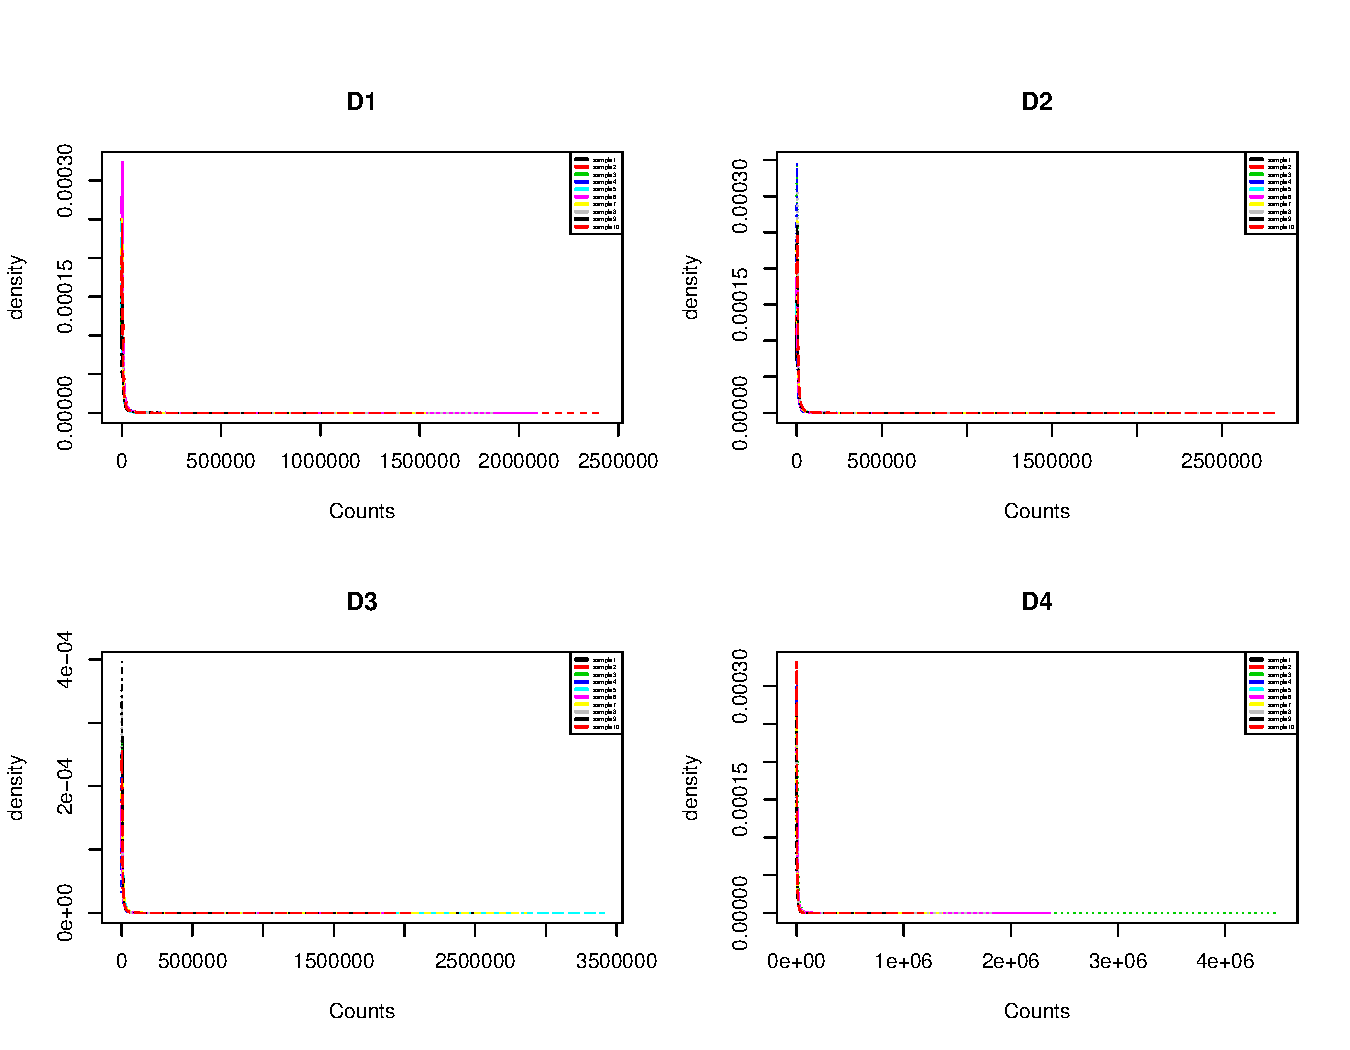
\includegraphics{Untitled_files/figure-latex/Observe count raw count distribution-1.pdf}

\begin{Shaded}
\begin{Highlighting}[]
\CommentTok{#Convert the dataset into an object that can be worked on by the vst function of Deseq2 package. This does not affect the data as the object created  has multiple slots including the original counts}
\NormalTok{Metadata <-}\StringTok{ }\KeywordTok{read.delim}\NormalTok{(}\KeywordTok{here}\NormalTok{(}\StringTok{"Project"}\NormalTok{,}\StringTok{"Metadata.txt"}\NormalTok{))}
\NormalTok{Metadata}\OperatorTok{$}\NormalTok{Groups <-}\StringTok{ }\KeywordTok{as.factor}\NormalTok{(Metadata}\OperatorTok{$}\NormalTok{Groups)}
\NormalTok{dds <-}\StringTok{ }\KeywordTok{DESeqDataSetFromMatrix}\NormalTok{(D1}\OperatorTok{@}\NormalTok{count.matrix, }
                              \DataTypeTok{colData =}\NormalTok{ Metadata, }
                              \DataTypeTok{design =} \OperatorTok{~}\NormalTok{Groups)}
\NormalTok{dds1 <-}\StringTok{ }\KeywordTok{DESeq}\NormalTok{(dds)}

\CommentTok{#Transform and plot the dataset}
\NormalTok{vsd <-}\StringTok{ }\KeywordTok{vst}\NormalTok{(dds1, }\DataTypeTok{blind=}\OtherTok{FALSE}\NormalTok{)}
\KeywordTok{head}\NormalTok{(}\KeywordTok{assay}\NormalTok{(vsd), }\DecValTok{3}\NormalTok{)}
\end{Highlighting}
\end{Shaded}

\begin{verbatim}
##     sample1  sample2  sample3  sample4  sample5  sample6  sample7  sample8
## g1 12.83999 12.63004 13.18539 12.85077 13.13527 13.43362 13.64820 13.11632
## g2 12.70894 11.17865 12.69099 10.89762 11.98284 14.46935 15.29341 12.61442
## g3 13.71002 12.61003 13.04778 12.95460 13.58159 14.23933 13.07089 15.09662
##     sample9 sample10
## g1 13.54991 13.30268
## g2 13.47458 15.21118
## g3 14.17843 13.70661
\end{verbatim}

\begin{Shaded}
\begin{Highlighting}[]
\NormalTok{sampleDists <-}\StringTok{ }\KeywordTok{dist}\NormalTok{(}\KeywordTok{t}\NormalTok{(}\KeywordTok{assay}\NormalTok{(vsd)))}

\NormalTok{sampleDistMatrix <-}\StringTok{ }\KeywordTok{as.matrix}\NormalTok{(sampleDists)}

\KeywordTok{rownames}\NormalTok{(sampleDistMatrix) <-}\StringTok{ }\KeywordTok{paste}\NormalTok{(vsd}\OperatorTok{$}\NormalTok{SampleID)}
\KeywordTok{colnames}\NormalTok{(sampleDistMatrix) <-}\StringTok{ }\OtherTok{NULL}
\NormalTok{colors <-}\StringTok{ }\KeywordTok{colorRampPalette}\NormalTok{( }\KeywordTok{rev}\NormalTok{(}\KeywordTok{brewer.pal}\NormalTok{(}\DecValTok{9}\NormalTok{, }\StringTok{"Blues"}\NormalTok{)) )(}\DecValTok{255}\NormalTok{)}
\KeywordTok{pheatmap}\NormalTok{(sampleDistMatrix,}
         \DataTypeTok{clustering_distance_rows=}\NormalTok{sampleDists,}
         \DataTypeTok{clustering_distance_cols=}\NormalTok{sampleDists,}\DataTypeTok{show_rownames =}\NormalTok{ T, }\DataTypeTok{show_colnames =}\NormalTok{ T,}
         \DataTypeTok{col=}\NormalTok{colors)}
\end{Highlighting}
\end{Shaded}

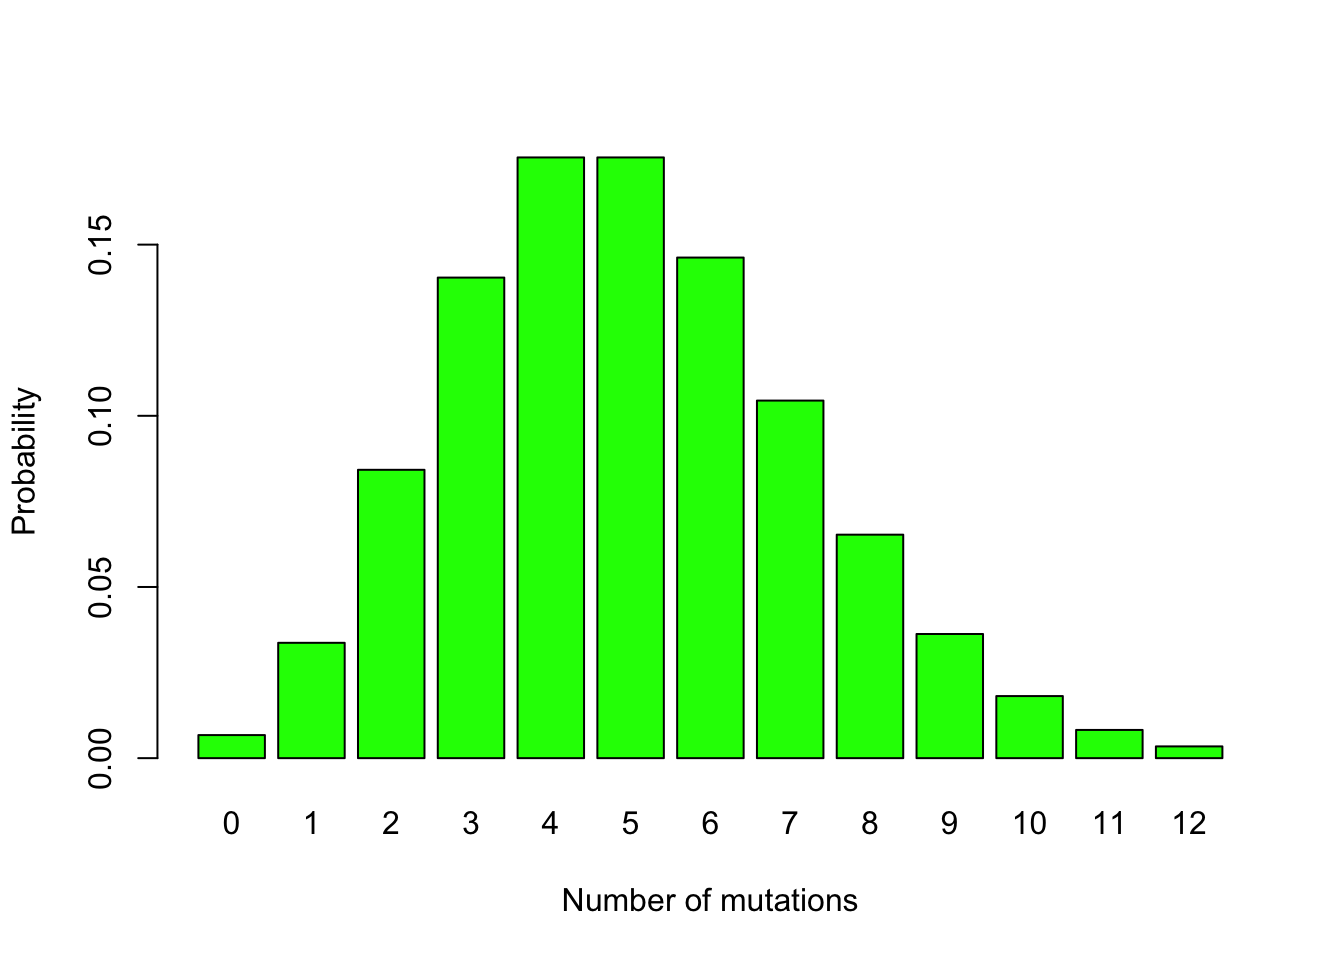
\includegraphics{Untitled_files/figure-latex/unnamed-chunk-2-1.pdf}

\begin{Shaded}
\begin{Highlighting}[]
\KeywordTok{plotPCA}\NormalTok{(vsd, }\DataTypeTok{intgroup=}\KeywordTok{c}\NormalTok{(}\StringTok{"Groups"}\NormalTok{))}
\end{Highlighting}
\end{Shaded}

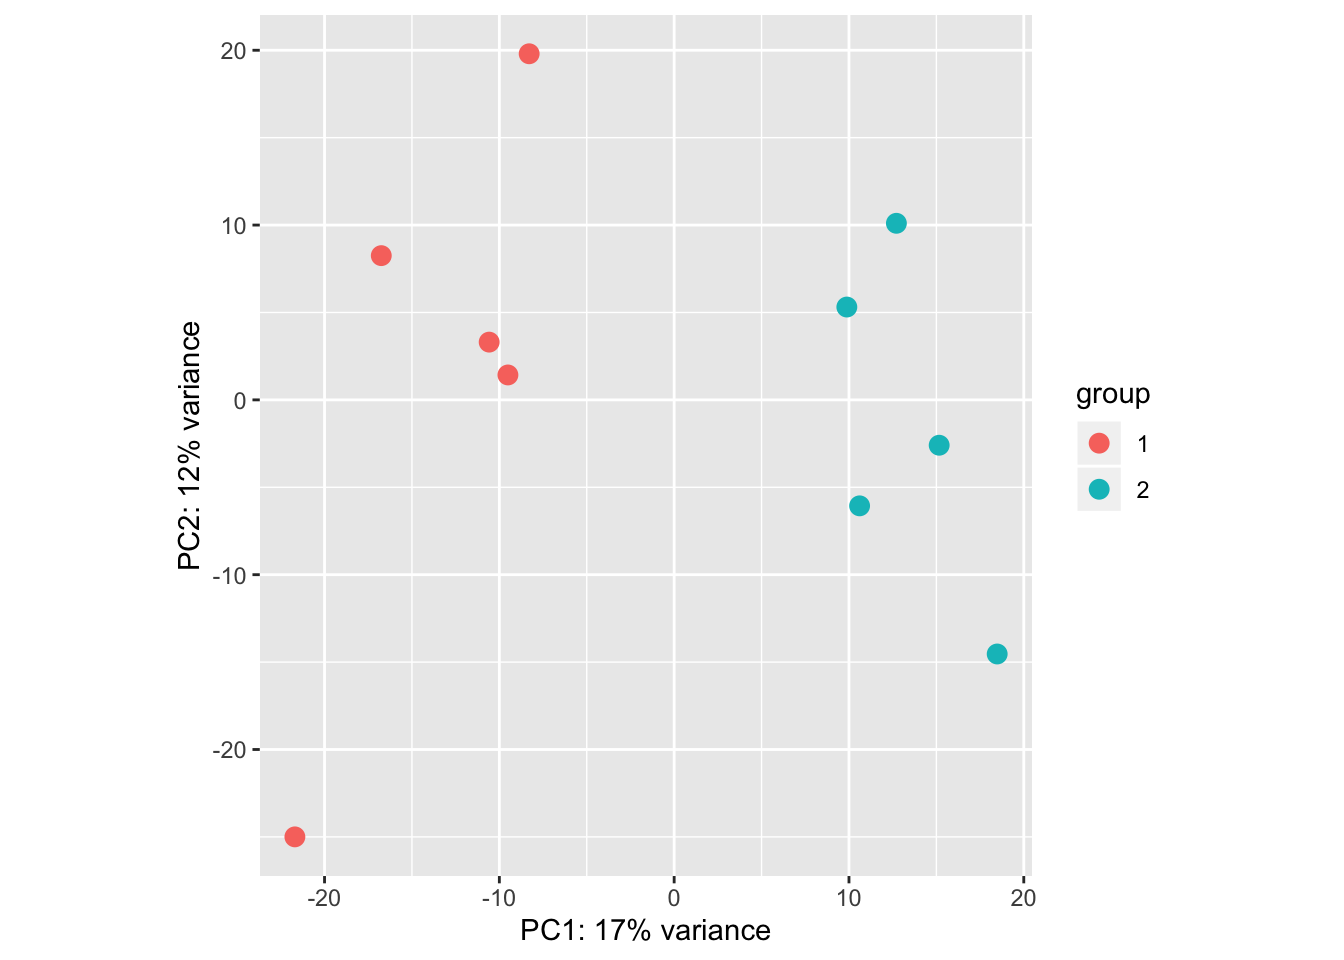
\includegraphics{Untitled_files/figure-latex/unnamed-chunk-2-2.pdf} \#\#
Differential expression

Three tools were compared; DESeq2, DEGseq, NOISeq. Analysis was executed
by following the guidelines available in the manuals of these tools. In
most cases, the default setting were followed except when there was a
need to do otherwise.

DESeq2: A DESeqDataSet object was created from the matrix of counts and
metadata using DESeqDataSetFromMatrix function for counts data. The
\emph{\emph{DESeq}} function was then run on the object created to
perform differential gene expression analysis. This was followed by
building the results table using the results function. MA plots were
then generated from the results obtained. Finally, selection of
differentially expressed genes was done, genes with adjusted p-values of
less than 0.05 were considered to be significantly differentially
expressed genes.

DEGseq: A DEGseq data object was created using \emph{readGeneExp}
function. The \emph{DEGexp} function was then run on the object created
to perform differential gene expression analysis with
\emph{thresholdKind} set to 3 (Benjamini adjusted q-value). As
recomnedaded by the authors, no normalization method was selected. A
graphical summary of the results was automatically generated. Finally,
genes with adjusted p-values less than 0.05 were considered to be
significantly differentially expressed genes.

NOISeq: \emph{noiseq} was run on a noiseq genertaed object from the
count matrix with the the trimmed mean of M normalization. A 0.8
threshold for the \(q\) statsitic was then used to select differentially
expressed genes.

Using the truth dataset from the simulated dataset, performance mersures
such as prescision, recall and F1-score were calculated. Venn diagrams
were generated with
\href{http://bioinformatics.psb.ugent.be/webtools/Venn/}{VennDiagrams}
online tool.

\begin{Shaded}
\begin{Highlighting}[]
\CommentTok{# Create the DESeqDataSet object from Matrix of counts and metadata}
\NormalTok{dds <-}\StringTok{ }\KeywordTok{DESeqDataSetFromMatrix}\NormalTok{(D1}\OperatorTok{@}\NormalTok{count.matrix, }
                              \DataTypeTok{colData =}\NormalTok{ Metadata, }
                              \DataTypeTok{design =} \OperatorTok{~}\NormalTok{Groups)}
\CommentTok{###Confirm that the rows of the deseq object is same as original data}
\KeywordTok{nrow}\NormalTok{(dds) }
\end{Highlighting}
\end{Shaded}

\begin{verbatim}
## [1] 12997
\end{verbatim}

\begin{Shaded}
\begin{Highlighting}[]
\CommentTok{#Run DESeq function on the data to perform differential gene expression analysis}
\NormalTok{dds1 <-}\StringTok{ }\KeywordTok{DESeq}\NormalTok{(dds)}

\CommentTok{##View the calculated size factors for each sample}
\KeywordTok{colData}\NormalTok{(dds1)}
\end{Highlighting}
\end{Shaded}

\begin{verbatim}
## DataFrame with 10 rows and 3 columns
##          SampleID   Groups        sizeFactor
##          <factor> <factor>         <numeric>
## sample1   sample1        1 0.850115064093275
## sample2   sample2        1  1.08856724881021
## sample3   sample3        1  1.39866716968907
## sample4   sample4        1 0.994468408151956
## sample5   sample5        1 0.768362038209123
## sample6   sample6        2  1.25433437017283
## sample7   sample7        2  1.08852844340515
## sample8   sample8        2 0.932091898146313
## sample9   sample9        2 0.801553920809952
## sample10 sample10        2  1.26644362287029
\end{verbatim}

\begin{Shaded}
\begin{Highlighting}[]
\CommentTok{# Build out results table}
\NormalTok{res <-}\StringTok{ }\KeywordTok{results}\NormalTok{(dds1)}
\KeywordTok{mcols}\NormalTok{(res , }\DataTypeTok{use.names=}\OtherTok{TRUE}\NormalTok{)}
\end{Highlighting}
\end{Shaded}

\begin{verbatim}
## DataFrame with 6 rows and 2 columns
##                        type                               description
##                 <character>                               <character>
## baseMean       intermediate mean of normalized counts for all samples
## log2FoldChange      results     log2 fold change (MLE): Groups 2 vs 1
## lfcSE               results             standard error: Groups 2 vs 1
## stat                results             Wald statistic: Groups 2 vs 1
## pvalue              results          Wald test p-value: Groups 2 vs 1
## padj                results                      BH adjusted p-values
\end{verbatim}

\begin{Shaded}
\begin{Highlighting}[]
\CommentTok{#Get a quick summary of the results}
\KeywordTok{summary}\NormalTok{(res )}
\end{Highlighting}
\end{Shaded}

\begin{verbatim}
## 
## out of 12997 with nonzero total read count
## adjusted p-value < 0.1
## LFC > 0 (up)       : 432, 3.3%
## LFC < 0 (down)     : 424, 3.3%
## outliers [1]       : 112, 0.86%
## low counts [2]     : 0, 0%
## (mean count < 0)
## [1] see 'cooksCutoff' argument of ?results
## [2] see 'independentFiltering' argument of ?results
\end{verbatim}

\begin{Shaded}
\begin{Highlighting}[]
\CommentTok{#Number of genes with padj < 0.05}
\KeywordTok{sum}\NormalTok{(res}\OperatorTok{$}\NormalTok{padj }\OperatorTok{<}\StringTok{ }\FloatTok{0.05}\NormalTok{, }\DataTypeTok{na.rm=}\OtherTok{TRUE}\NormalTok{)}
\end{Highlighting}
\end{Shaded}

\begin{verbatim}
## [1] 703
\end{verbatim}

\begin{Shaded}
\begin{Highlighting}[]
\CommentTok{#MA Plot on before and after apeglm shrinkage"}
\NormalTok{resLFC <-}\StringTok{ }\KeywordTok{lfcShrink}\NormalTok{(dds1, }\DataTypeTok{coef=}\DecValTok{2}\NormalTok{, }\DataTypeTok{type=}\StringTok{"apeglm"}\NormalTok{)}
\KeywordTok{par}\NormalTok{(}\DataTypeTok{mfrow=}\KeywordTok{c}\NormalTok{(}\DecValTok{1}\NormalTok{,}\DecValTok{2}\NormalTok{))}

\KeywordTok{plotMA}\NormalTok{(res,}\DataTypeTok{main =} \StringTok{"MA Plot of D1"}\NormalTok{,}\DataTypeTok{xlab =}\StringTok{"Mean of Normalised counts"}\NormalTok{,}
       \DataTypeTok{xlim=}\KeywordTok{c}\NormalTok{(}\DecValTok{1}\NormalTok{,}\DecValTok{150000}\NormalTok{), }\DataTypeTok{ylim=}\KeywordTok{c}\NormalTok{(}\OperatorTok{-}\DecValTok{6}\NormalTok{,}\DecValTok{6}\NormalTok{))}
\KeywordTok{plotMA}\NormalTok{(resLFC, }\DataTypeTok{xlim=}\KeywordTok{c}\NormalTok{(}\DecValTok{1}\NormalTok{,}\DecValTok{150000}\NormalTok{), }\DataTypeTok{ylim=}\KeywordTok{c}\NormalTok{(}\OperatorTok{-}\DecValTok{6}\NormalTok{,}\DecValTok{6}\NormalTok{),}\DataTypeTok{xlab=}\StringTok{"Mean of Normalised counts"}\NormalTok{, }\DataTypeTok{main=}\StringTok{"apeglm"}\NormalTok{)}
\end{Highlighting}
\end{Shaded}

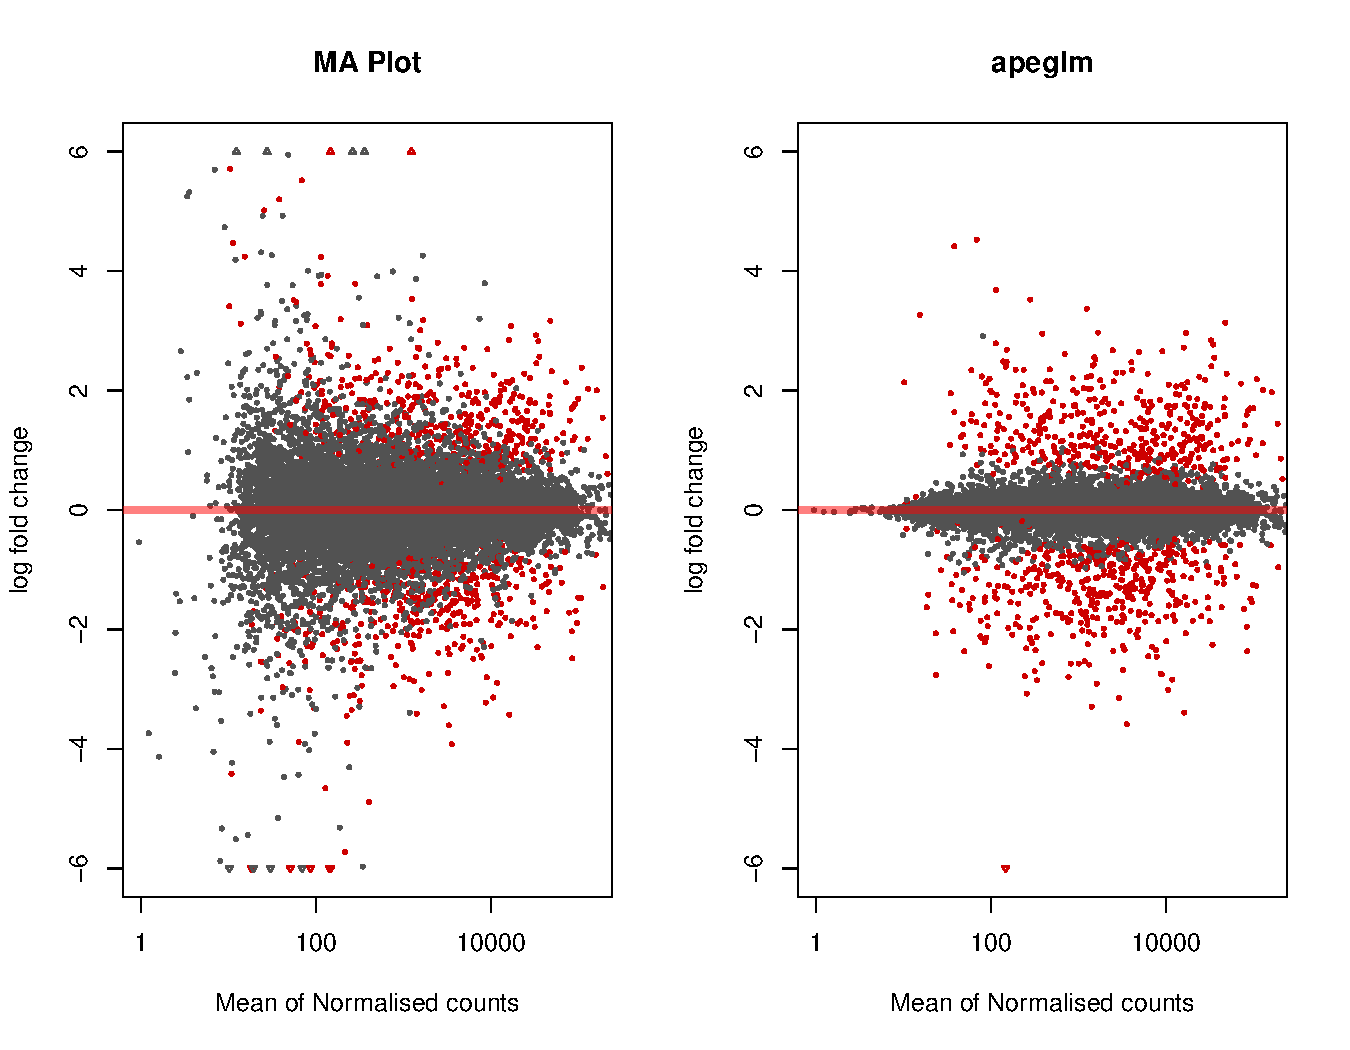
\includegraphics{Untitled_files/figure-latex/Deseq2-1.pdf}

\begin{Shaded}
\begin{Highlighting}[]
\CommentTok{#Working with alpha 0.05}
\NormalTok{res05_D1 <-}\StringTok{ }\KeywordTok{results}\NormalTok{(dds1, }\DataTypeTok{alpha=}\FloatTok{0.05}\NormalTok{)}
\KeywordTok{summary}\NormalTok{(res05_D1)}
\end{Highlighting}
\end{Shaded}

\begin{verbatim}
## 
## out of 12997 with nonzero total read count
## adjusted p-value < 0.05
## LFC > 0 (up)       : 351, 2.7%
## LFC < 0 (down)     : 352, 2.7%
## outliers [1]       : 112, 0.86%
## low counts [2]     : 0, 0%
## (mean count < 0)
## [1] see 'cooksCutoff' argument of ?results
## [2] see 'independentFiltering' argument of ?results
\end{verbatim}

\begin{Shaded}
\begin{Highlighting}[]
\CommentTok{#You can select the gene to plot by rowname or by numeric index.}
\KeywordTok{par}\NormalTok{(}\DataTypeTok{mfrow=}\KeywordTok{c}\NormalTok{(}\DecValTok{1}\NormalTok{,}\DecValTok{1}\NormalTok{))}
\KeywordTok{plotCounts}\NormalTok{(dds1, }\DataTypeTok{gene=}\KeywordTok{which.min}\NormalTok{(res05_D1}\OperatorTok{$}\NormalTok{padj), }\DataTypeTok{intgroup=}\StringTok{"Groups"}\NormalTok{)}
\end{Highlighting}
\end{Shaded}

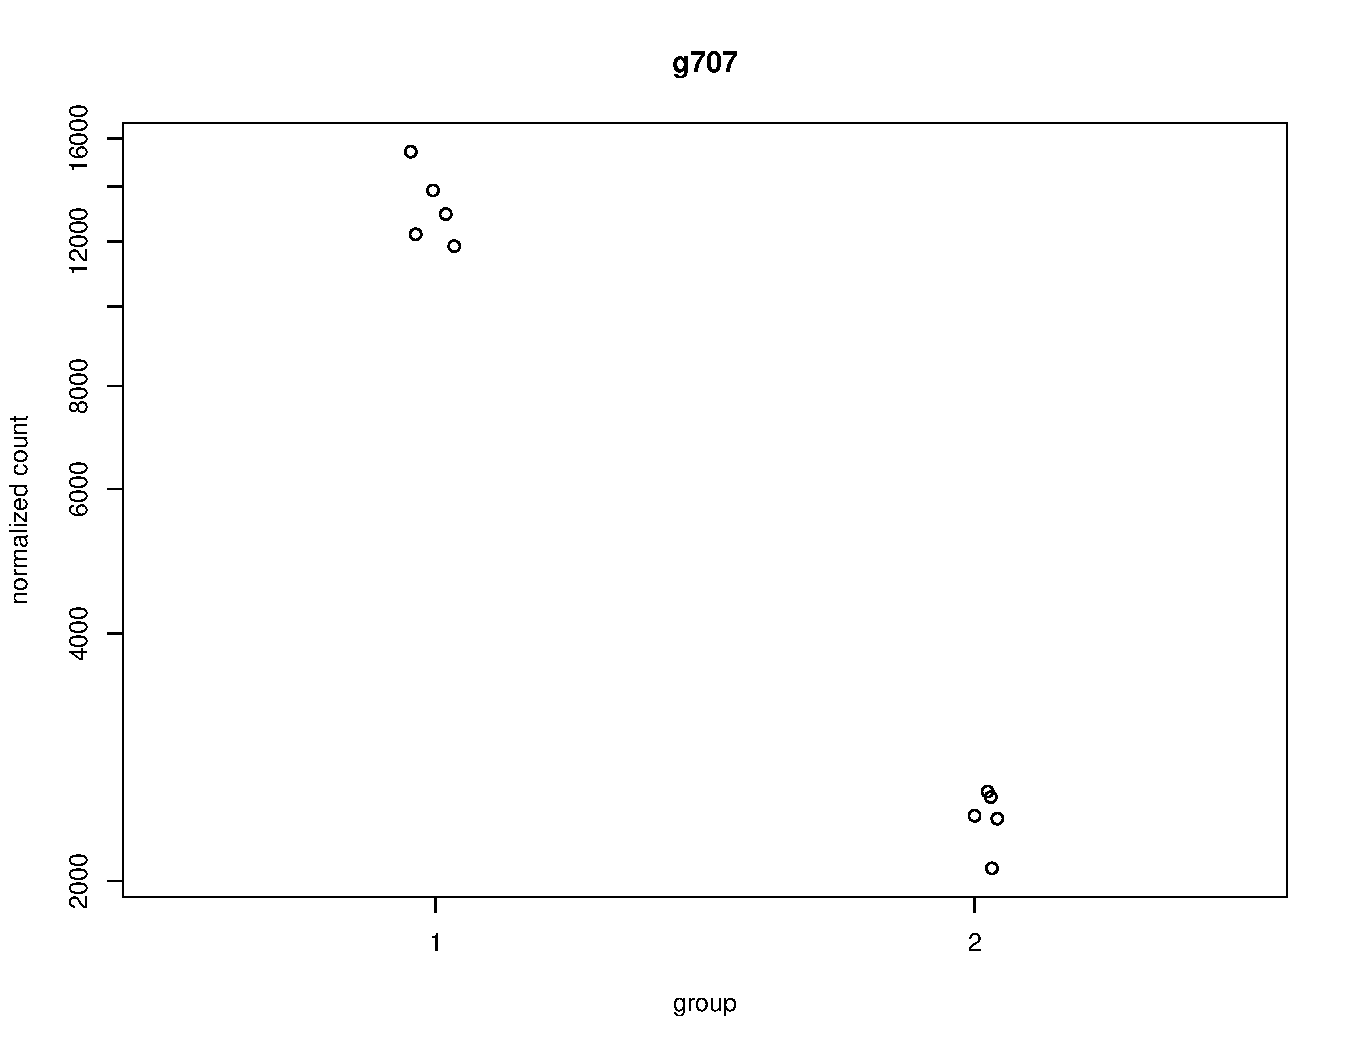
\includegraphics{Untitled_files/figure-latex/Deseq2-2.pdf}

\begin{Shaded}
\begin{Highlighting}[]
\CommentTok{#Select genes with padj < 0.05 }
\NormalTok{resSig_D1 <-}\StringTok{ }\KeywordTok{subset}\NormalTok{(res05_D1, padj }\OperatorTok{<}\StringTok{ }\FloatTok{0.05}\NormalTok{)}
\KeywordTok{nrow}\NormalTok{(resSig_D1)}
\end{Highlighting}
\end{Shaded}

\begin{verbatim}
## [1] 703
\end{verbatim}

\begin{Shaded}
\begin{Highlighting}[]
\KeywordTok{write.csv}\NormalTok{(resSig_D1,}\StringTok{'DEseq2_D1_res.csv'}\NormalTok{)}



\CommentTok{#Do same for all four datasets}
\CommentTok{##For D2}
\NormalTok{dds2 <-}\StringTok{ }\KeywordTok{DESeqDataSetFromMatrix}\NormalTok{(D2}\OperatorTok{@}\NormalTok{count.matrix, }
                              \DataTypeTok{colData =}\NormalTok{ Metadata, }
                              \DataTypeTok{design =} \OperatorTok{~}\NormalTok{Groups)}
\KeywordTok{nrow}\NormalTok{(dds2) }
\end{Highlighting}
\end{Shaded}

\begin{verbatim}
## [1] 12998
\end{verbatim}

\begin{Shaded}
\begin{Highlighting}[]
\NormalTok{dds2 <-}\StringTok{ }\KeywordTok{DESeq}\NormalTok{(dds2)}
\KeywordTok{colData}\NormalTok{(dds2)}
\end{Highlighting}
\end{Shaded}

\begin{verbatim}
## DataFrame with 10 rows and 3 columns
##          SampleID   Groups        sizeFactor
##          <factor> <factor>         <numeric>
## sample1   sample1        1 0.779448037475267
## sample2   sample2        1  1.22827700726851
## sample3   sample3        1  1.06879532655364
## sample4   sample4        1 0.722716378616827
## sample5   sample5        1 0.938326190354225
## sample6   sample6        2  1.05121341884108
## sample7   sample7        2  1.24577246907866
## sample8   sample8        2  1.26873134562723
## sample9   sample9        2  1.22035050540828
## sample10 sample10        2 0.911421482868434
\end{verbatim}

\begin{Shaded}
\begin{Highlighting}[]
\NormalTok{res2 <-}\StringTok{ }\KeywordTok{results}\NormalTok{(dds2)}
\KeywordTok{mcols}\NormalTok{(res2 , }\DataTypeTok{use.names=}\OtherTok{TRUE}\NormalTok{)}
\end{Highlighting}
\end{Shaded}

\begin{verbatim}
## DataFrame with 6 rows and 2 columns
##                        type                               description
##                 <character>                               <character>
## baseMean       intermediate mean of normalized counts for all samples
## log2FoldChange      results     log2 fold change (MLE): Groups 2 vs 1
## lfcSE               results             standard error: Groups 2 vs 1
## stat                results             Wald statistic: Groups 2 vs 1
## pvalue              results          Wald test p-value: Groups 2 vs 1
## padj                results                      BH adjusted p-values
\end{verbatim}

\begin{Shaded}
\begin{Highlighting}[]
\KeywordTok{summary}\NormalTok{(res2 )}
\end{Highlighting}
\end{Shaded}

\begin{verbatim}
## 
## out of 12998 with nonzero total read count
## adjusted p-value < 0.1
## LFC > 0 (up)       : 451, 3.5%
## LFC < 0 (down)     : 428, 3.3%
## outliers [1]       : 100, 0.77%
## low counts [2]     : 0, 0%
## (mean count < 0)
## [1] see 'cooksCutoff' argument of ?results
## [2] see 'independentFiltering' argument of ?results
\end{verbatim}

\begin{Shaded}
\begin{Highlighting}[]
\KeywordTok{sum}\NormalTok{(res2}\OperatorTok{$}\NormalTok{padj }\OperatorTok{<}\StringTok{ }\FloatTok{0.05}\NormalTok{, }\DataTypeTok{na.rm=}\OtherTok{TRUE}\NormalTok{)}
\end{Highlighting}
\end{Shaded}

\begin{verbatim}
## [1] 716
\end{verbatim}

\begin{Shaded}
\begin{Highlighting}[]
\NormalTok{resLFC2 <-}\StringTok{ }\KeywordTok{lfcShrink}\NormalTok{(dds2, }\DataTypeTok{coef=}\DecValTok{2}\NormalTok{, }\DataTypeTok{type=}\StringTok{"apeglm"}\NormalTok{)}
\KeywordTok{par}\NormalTok{(}\DataTypeTok{mfrow=}\KeywordTok{c}\NormalTok{(}\DecValTok{1}\NormalTok{,}\DecValTok{2}\NormalTok{))}
\KeywordTok{plotMA}\NormalTok{(res2,}\DataTypeTok{main =} \StringTok{"MA Plot of D2"}\NormalTok{,}\DataTypeTok{xlab =}\StringTok{"Mean of Normalised counts"}\NormalTok{, }\DataTypeTok{xlim=}\KeywordTok{c}\NormalTok{(}\DecValTok{1}\NormalTok{,}\DecValTok{150000}\NormalTok{), }\DataTypeTok{ylim=}\KeywordTok{c}\NormalTok{(}\OperatorTok{-}\DecValTok{6}\NormalTok{,}\DecValTok{6}\NormalTok{))}
\KeywordTok{plotMA}\NormalTok{(resLFC2, }\DataTypeTok{xlim=}\KeywordTok{c}\NormalTok{(}\DecValTok{1}\NormalTok{,}\DecValTok{150000}\NormalTok{), }\DataTypeTok{ylim=}\KeywordTok{c}\NormalTok{(}\OperatorTok{-}\DecValTok{6}\NormalTok{,}\DecValTok{6}\NormalTok{),}\DataTypeTok{xlab=}\StringTok{"Mean of Normalised counts"}\NormalTok{, }\DataTypeTok{main=}\StringTok{"apeglm"}\NormalTok{)}
\end{Highlighting}
\end{Shaded}

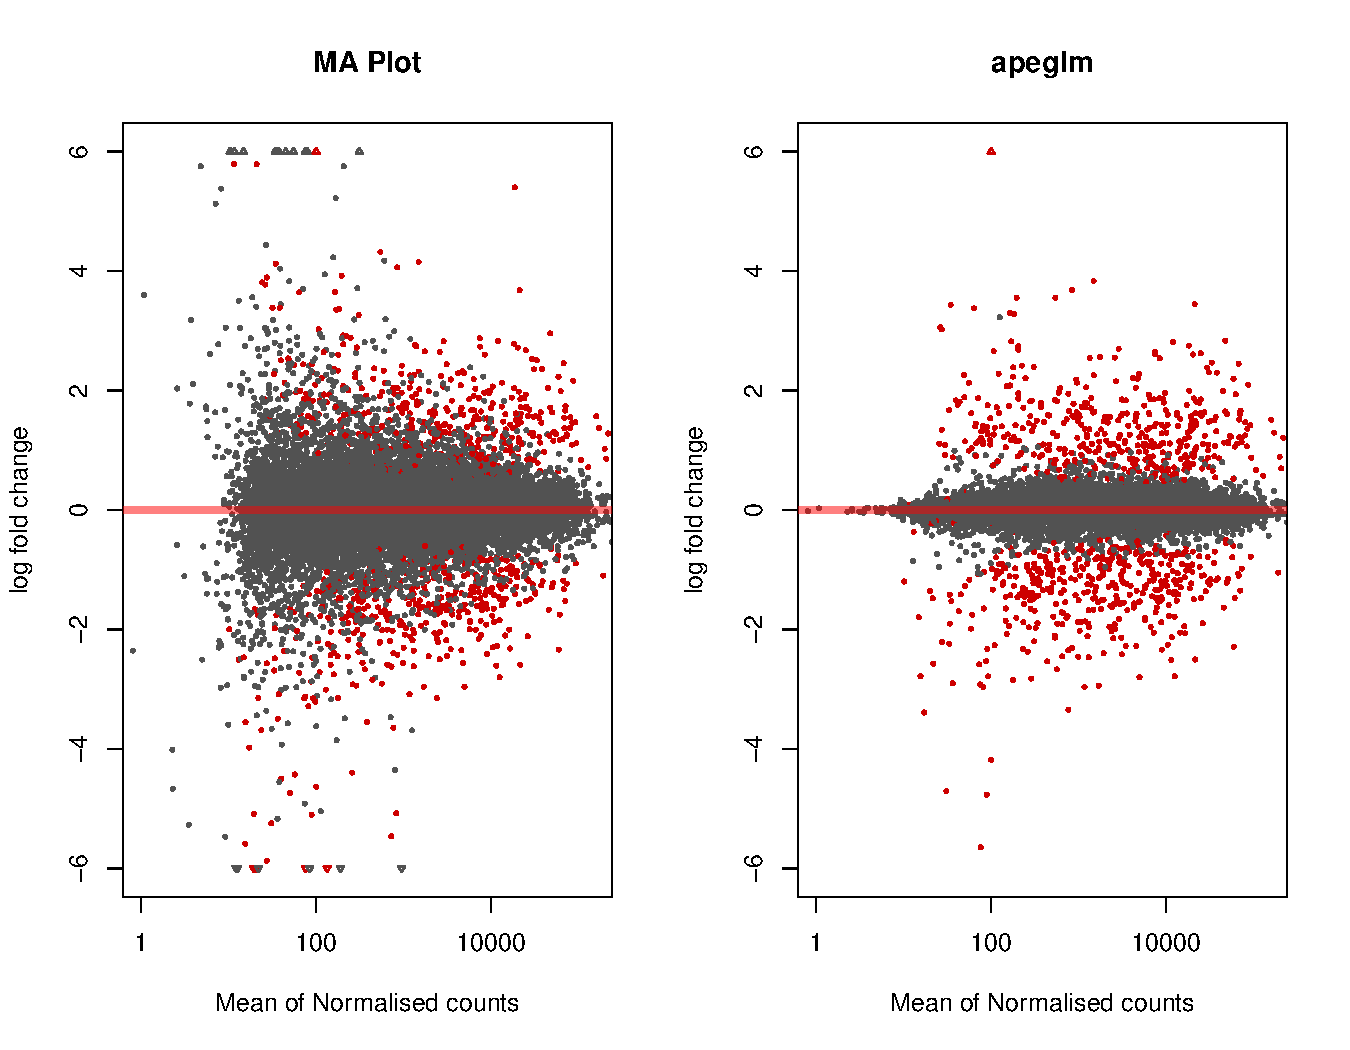
\includegraphics{Untitled_files/figure-latex/Deseq2-3.pdf}

\begin{Shaded}
\begin{Highlighting}[]
\NormalTok{res05_D2 <-}\StringTok{ }\KeywordTok{results}\NormalTok{(dds2, }\DataTypeTok{alpha=}\FloatTok{0.05}\NormalTok{)}
\KeywordTok{summary}\NormalTok{(res05_D2)}
\end{Highlighting}
\end{Shaded}

\begin{verbatim}
## 
## out of 12998 with nonzero total read count
## adjusted p-value < 0.05
## LFC > 0 (up)       : 370, 2.8%
## LFC < 0 (down)     : 346, 2.7%
## outliers [1]       : 100, 0.77%
## low counts [2]     : 0, 0%
## (mean count < 0)
## [1] see 'cooksCutoff' argument of ?results
## [2] see 'independentFiltering' argument of ?results
\end{verbatim}

\begin{Shaded}
\begin{Highlighting}[]
\KeywordTok{par}\NormalTok{(}\DataTypeTok{mfrow=}\KeywordTok{c}\NormalTok{(}\DecValTok{1}\NormalTok{,}\DecValTok{1}\NormalTok{))}
\KeywordTok{plotCounts}\NormalTok{(dds2, }\DataTypeTok{gene=}\KeywordTok{which.min}\NormalTok{(res2}\OperatorTok{$}\NormalTok{padj), }\DataTypeTok{intgroup=}\StringTok{"Groups"}\NormalTok{)}
\end{Highlighting}
\end{Shaded}

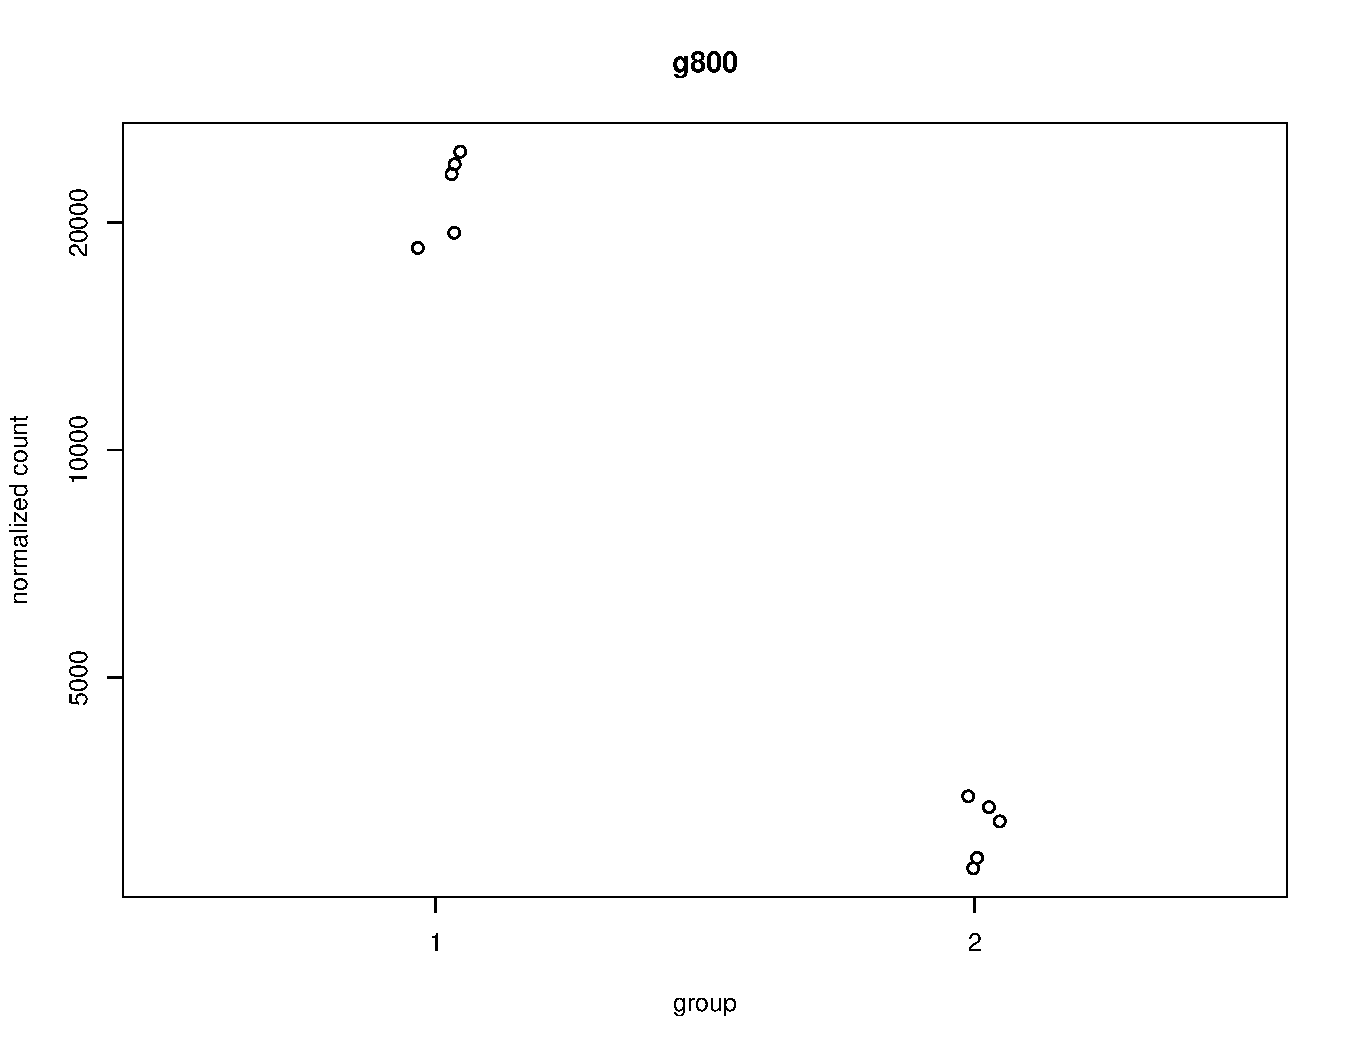
\includegraphics{Untitled_files/figure-latex/Deseq2-4.pdf}

\begin{Shaded}
\begin{Highlighting}[]
\NormalTok{resSig_D2 <-}\StringTok{ }\KeywordTok{subset}\NormalTok{(res05_D2, padj }\OperatorTok{<}\StringTok{ }\FloatTok{0.05}\NormalTok{)}
\KeywordTok{nrow}\NormalTok{(resSig_D2)}
\end{Highlighting}
\end{Shaded}

\begin{verbatim}
## [1] 716
\end{verbatim}

\begin{Shaded}
\begin{Highlighting}[]
\KeywordTok{write.csv}\NormalTok{(resSig_D2,}\StringTok{'DEseq2_D2_res.csv'}\NormalTok{)}


\CommentTok{##For D3}
\NormalTok{dds3 <-}\StringTok{ }\KeywordTok{DESeqDataSetFromMatrix}\NormalTok{(D3}\OperatorTok{@}\NormalTok{count.matrix, }
                              \DataTypeTok{colData =}\NormalTok{ Metadata, }
                              \DataTypeTok{design =} \OperatorTok{~}\NormalTok{Groups)}
\KeywordTok{nrow}\NormalTok{(dds3) }
\end{Highlighting}
\end{Shaded}

\begin{verbatim}
## [1] 12999
\end{verbatim}

\begin{Shaded}
\begin{Highlighting}[]
\NormalTok{dds3 <-}\StringTok{ }\KeywordTok{DESeq}\NormalTok{(dds3)}
\KeywordTok{colData}\NormalTok{(dds3)}
\end{Highlighting}
\end{Shaded}

\begin{verbatim}
## DataFrame with 10 rows and 3 columns
##          SampleID   Groups        sizeFactor
##          <factor> <factor>         <numeric>
## sample1   sample1        1 0.993104153321671
## sample2   sample2        1  1.35152809757693
## sample3   sample3        1 0.876006961778257
## sample4   sample4        1  0.93119949319263
## sample5   sample5        1 0.832001628273773
## sample6   sample6        2  1.21688047873468
## sample7   sample7        2  1.00522030917127
## sample8   sample8        2  1.21533585508711
## sample9   sample9        2 0.912212289090538
## sample10 sample10        2  1.05769664760319
\end{verbatim}

\begin{Shaded}
\begin{Highlighting}[]
\NormalTok{res3 <-}\StringTok{ }\KeywordTok{results}\NormalTok{(dds3)}
\KeywordTok{mcols}\NormalTok{(res3 , }\DataTypeTok{use.names=}\OtherTok{TRUE}\NormalTok{)}
\end{Highlighting}
\end{Shaded}

\begin{verbatim}
## DataFrame with 6 rows and 2 columns
##                        type                               description
##                 <character>                               <character>
## baseMean       intermediate mean of normalized counts for all samples
## log2FoldChange      results     log2 fold change (MLE): Groups 2 vs 1
## lfcSE               results             standard error: Groups 2 vs 1
## stat                results             Wald statistic: Groups 2 vs 1
## pvalue              results          Wald test p-value: Groups 2 vs 1
## padj                results                      BH adjusted p-values
\end{verbatim}

\begin{Shaded}
\begin{Highlighting}[]
\KeywordTok{summary}\NormalTok{(res3)}
\end{Highlighting}
\end{Shaded}

\begin{verbatim}
## 
## out of 12999 with nonzero total read count
## adjusted p-value < 0.1
## LFC > 0 (up)       : 467, 3.6%
## LFC < 0 (down)     : 452, 3.5%
## outliers [1]       : 121, 0.93%
## low counts [2]     : 0, 0%
## (mean count < 0)
## [1] see 'cooksCutoff' argument of ?results
## [2] see 'independentFiltering' argument of ?results
\end{verbatim}

\begin{Shaded}
\begin{Highlighting}[]
\KeywordTok{sum}\NormalTok{(res3}\OperatorTok{$}\NormalTok{padj }\OperatorTok{<}\StringTok{ }\FloatTok{0.05}\NormalTok{, }\DataTypeTok{na.rm=}\OtherTok{TRUE}\NormalTok{)}
\end{Highlighting}
\end{Shaded}

\begin{verbatim}
## [1] 758
\end{verbatim}

\begin{Shaded}
\begin{Highlighting}[]
\NormalTok{resLFC3 <-}\StringTok{ }\KeywordTok{lfcShrink}\NormalTok{(dds3, }\DataTypeTok{coef=}\DecValTok{2}\NormalTok{, }\DataTypeTok{type=}\StringTok{"apeglm"}\NormalTok{)}
\KeywordTok{par}\NormalTok{(}\DataTypeTok{mfrow=}\KeywordTok{c}\NormalTok{(}\DecValTok{1}\NormalTok{,}\DecValTok{2}\NormalTok{))}
\KeywordTok{plotMA}\NormalTok{(res3,}\DataTypeTok{main =} \StringTok{"MA Plot of D3"}\NormalTok{,}\DataTypeTok{xlab =}\StringTok{"Mean of Normalised counts"}\NormalTok{,}
       \DataTypeTok{xlim=}\KeywordTok{c}\NormalTok{(}\DecValTok{1}\NormalTok{,}\DecValTok{150000}\NormalTok{), }\DataTypeTok{ylim=}\KeywordTok{c}\NormalTok{(}\OperatorTok{-}\DecValTok{6}\NormalTok{,}\DecValTok{6}\NormalTok{))}
\KeywordTok{plotMA}\NormalTok{(resLFC3, }\DataTypeTok{xlim=}\KeywordTok{c}\NormalTok{(}\DecValTok{1}\NormalTok{,}\DecValTok{150000}\NormalTok{), }\DataTypeTok{ylim=}\KeywordTok{c}\NormalTok{(}\OperatorTok{-}\DecValTok{6}\NormalTok{,}\DecValTok{6}\NormalTok{),}\DataTypeTok{xlab=}\StringTok{"Mean of Normalised counts"}\NormalTok{, }\DataTypeTok{main=}\StringTok{"apeglm"}\NormalTok{)}
\end{Highlighting}
\end{Shaded}

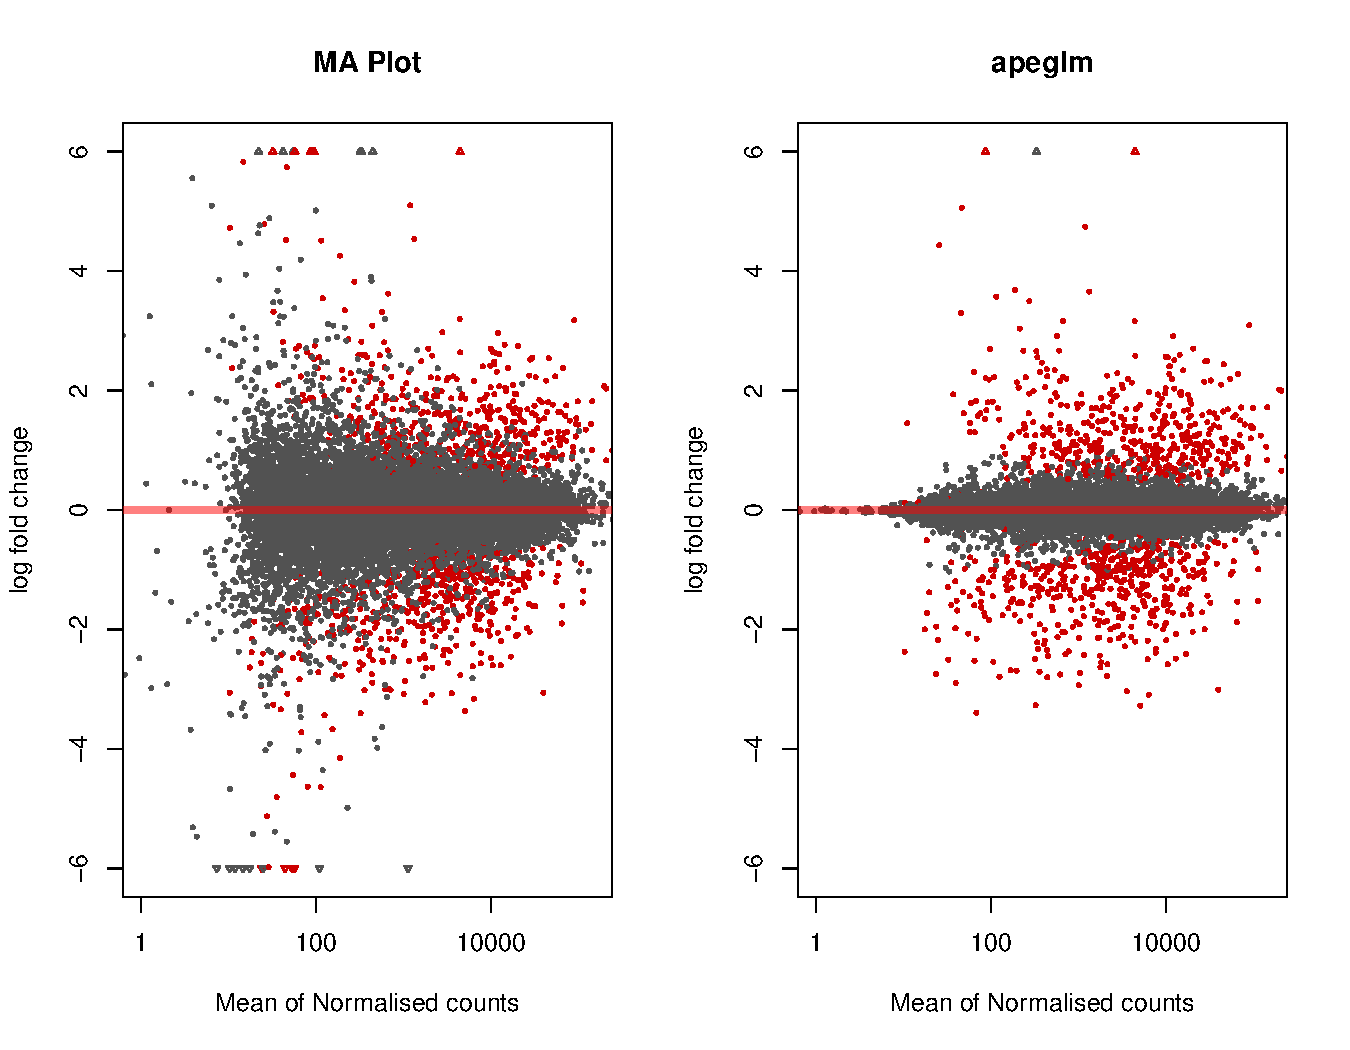
\includegraphics{Untitled_files/figure-latex/Deseq2-5.pdf}

\begin{Shaded}
\begin{Highlighting}[]
\NormalTok{res05_D3 <-}\StringTok{ }\KeywordTok{results}\NormalTok{(dds3, }\DataTypeTok{alpha=}\FloatTok{0.05}\NormalTok{)}
\KeywordTok{summary}\NormalTok{(res05_D3)}
\end{Highlighting}
\end{Shaded}

\begin{verbatim}
## 
## out of 12999 with nonzero total read count
## adjusted p-value < 0.05
## LFC > 0 (up)       : 387, 3%
## LFC < 0 (down)     : 375, 2.9%
## outliers [1]       : 121, 0.93%
## low counts [2]     : 226, 1.7%
## (mean count < 17)
## [1] see 'cooksCutoff' argument of ?results
## [2] see 'independentFiltering' argument of ?results
\end{verbatim}

\begin{Shaded}
\begin{Highlighting}[]
\KeywordTok{par}\NormalTok{(}\DataTypeTok{mfrow=}\KeywordTok{c}\NormalTok{(}\DecValTok{1}\NormalTok{,}\DecValTok{1}\NormalTok{))}
\KeywordTok{plotCounts}\NormalTok{(dds3, }\DataTypeTok{gene=}\KeywordTok{which.min}\NormalTok{(res3}\OperatorTok{$}\NormalTok{padj), }\DataTypeTok{intgroup=}\StringTok{"Groups"}\NormalTok{)}
\end{Highlighting}
\end{Shaded}

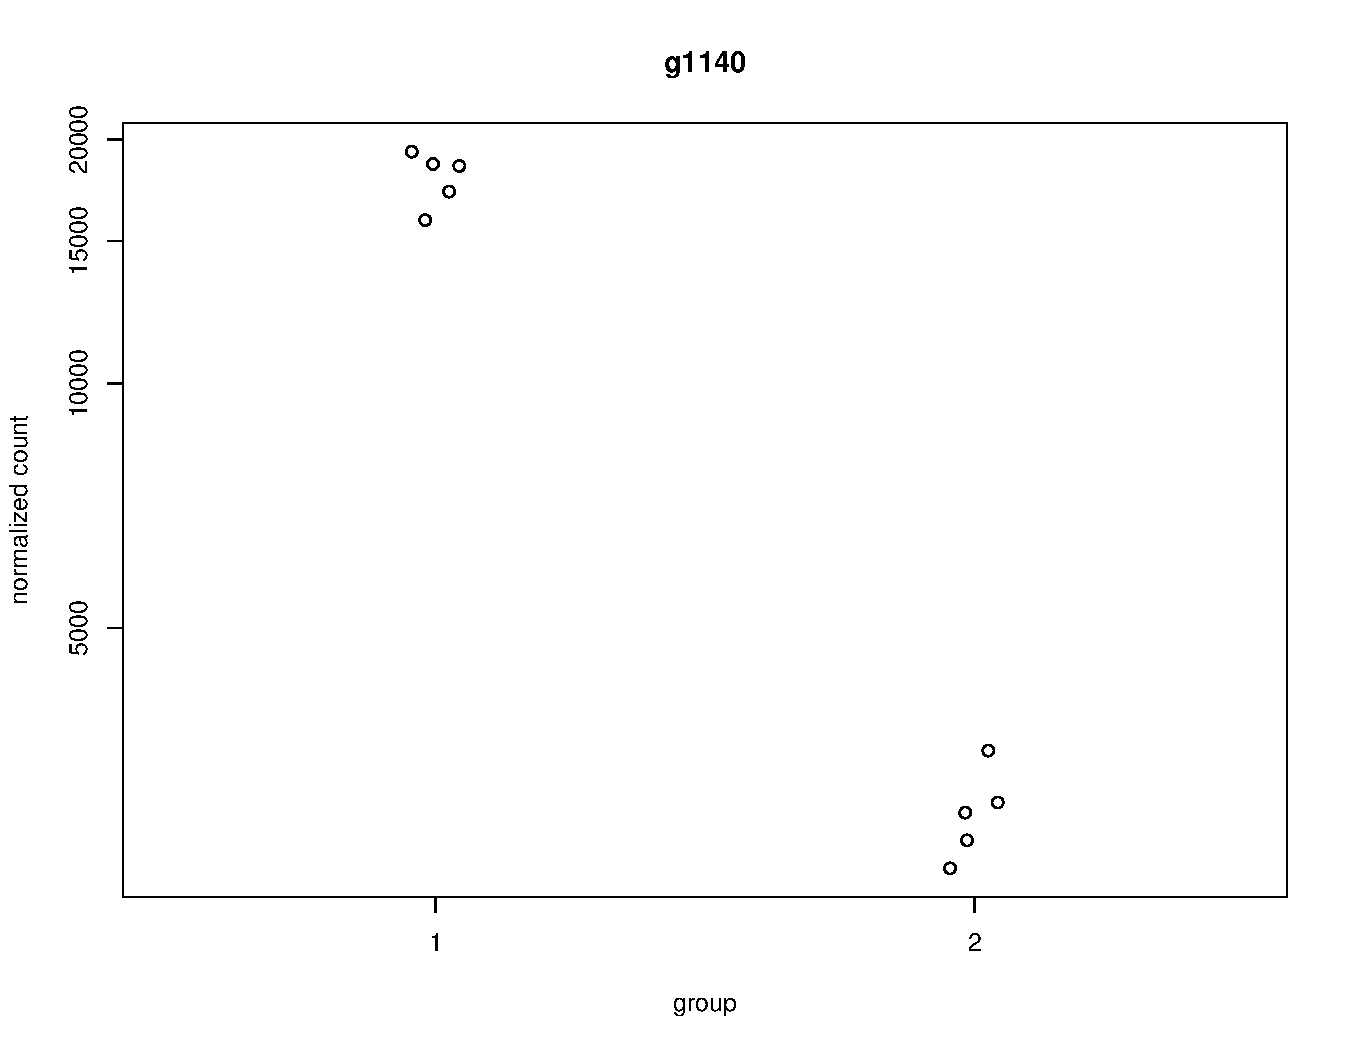
\includegraphics{Untitled_files/figure-latex/Deseq2-6.pdf}

\begin{Shaded}
\begin{Highlighting}[]
\NormalTok{resSig_D3 <-}\StringTok{ }\KeywordTok{subset}\NormalTok{(res05_D3, padj }\OperatorTok{<}\StringTok{ }\FloatTok{0.05}\NormalTok{)}
\KeywordTok{nrow}\NormalTok{(resSig_D3)}
\end{Highlighting}
\end{Shaded}

\begin{verbatim}
## [1] 762
\end{verbatim}

\begin{Shaded}
\begin{Highlighting}[]
\KeywordTok{write.csv}\NormalTok{(resSig_D3,}\StringTok{'DEseq2_D3_res.csv'}\NormalTok{)}


\CommentTok{##For D4}
\NormalTok{dds4 <-}\StringTok{ }\KeywordTok{DESeqDataSetFromMatrix}\NormalTok{(D4}\OperatorTok{@}\NormalTok{count.matrix, }
                              \DataTypeTok{colData =}\NormalTok{ Metadata, }
                              \DataTypeTok{design =} \OperatorTok{~}\NormalTok{Groups)}
\KeywordTok{nrow}\NormalTok{(dds4) }
\end{Highlighting}
\end{Shaded}

\begin{verbatim}
## [1] 12999
\end{verbatim}

\begin{Shaded}
\begin{Highlighting}[]
\NormalTok{dds4 <-}\StringTok{ }\KeywordTok{DESeq}\NormalTok{(dds4)}
\KeywordTok{colData}\NormalTok{(dds4)}
\end{Highlighting}
\end{Shaded}

\begin{verbatim}
## DataFrame with 10 rows and 3 columns
##          SampleID   Groups        sizeFactor
##          <factor> <factor>         <numeric>
## sample1   sample1        1 0.975625878873304
## sample2   sample2        1  1.15383733436947
## sample3   sample3        1  1.09936565349812
## sample4   sample4        1 0.940716375687604
## sample5   sample5        1 0.863125022987744
## sample6   sample6        2  1.10740071938824
## sample7   sample7        2 0.871063637714829
## sample8   sample8        2  1.08252297981681
## sample9   sample9        2 0.976725611615208
## sample10 sample10        2  1.26274563260039
\end{verbatim}

\begin{Shaded}
\begin{Highlighting}[]
\NormalTok{res4 <-}\StringTok{ }\KeywordTok{results}\NormalTok{(dds4)}
\KeywordTok{mcols}\NormalTok{(res4 , }\DataTypeTok{use.names=}\OtherTok{TRUE}\NormalTok{)}
\end{Highlighting}
\end{Shaded}

\begin{verbatim}
## DataFrame with 6 rows and 2 columns
##                        type                               description
##                 <character>                               <character>
## baseMean       intermediate mean of normalized counts for all samples
## log2FoldChange      results     log2 fold change (MLE): Groups 2 vs 1
## lfcSE               results             standard error: Groups 2 vs 1
## stat                results             Wald statistic: Groups 2 vs 1
## pvalue              results          Wald test p-value: Groups 2 vs 1
## padj                results                      BH adjusted p-values
\end{verbatim}

\begin{Shaded}
\begin{Highlighting}[]
\KeywordTok{summary}\NormalTok{(res4 )}
\end{Highlighting}
\end{Shaded}

\begin{verbatim}
## 
## out of 12999 with nonzero total read count
## adjusted p-value < 0.1
## LFC > 0 (up)       : 473, 3.6%
## LFC < 0 (down)     : 447, 3.4%
## outliers [1]       : 95, 0.73%
## low counts [2]     : 0, 0%
## (mean count < 0)
## [1] see 'cooksCutoff' argument of ?results
## [2] see 'independentFiltering' argument of ?results
\end{verbatim}

\begin{Shaded}
\begin{Highlighting}[]
\KeywordTok{sum}\NormalTok{(res4}\OperatorTok{$}\NormalTok{padj }\OperatorTok{<}\StringTok{ }\FloatTok{0.05}\NormalTok{, }\DataTypeTok{na.rm=}\OtherTok{TRUE}\NormalTok{)}
\end{Highlighting}
\end{Shaded}

\begin{verbatim}
## [1] 763
\end{verbatim}

\begin{Shaded}
\begin{Highlighting}[]
\NormalTok{resLFC4 <-}\StringTok{ }\KeywordTok{lfcShrink}\NormalTok{(dds4, }\DataTypeTok{coef=}\DecValTok{2}\NormalTok{, }\DataTypeTok{type=}\StringTok{"apeglm"}\NormalTok{)}
\KeywordTok{par}\NormalTok{(}\DataTypeTok{mfrow=}\KeywordTok{c}\NormalTok{(}\DecValTok{1}\NormalTok{,}\DecValTok{2}\NormalTok{))}
\KeywordTok{plotMA}\NormalTok{(res4,}\DataTypeTok{main =} \StringTok{"MA Plot of D4"}\NormalTok{,}\DataTypeTok{xlab =}\StringTok{"Mean of Normalised counts"}\NormalTok{,}
       \DataTypeTok{xlim=}\KeywordTok{c}\NormalTok{(}\DecValTok{1}\NormalTok{,}\DecValTok{150000}\NormalTok{), }\DataTypeTok{ylim=}\KeywordTok{c}\NormalTok{(}\OperatorTok{-}\DecValTok{6}\NormalTok{,}\DecValTok{6}\NormalTok{))}
\KeywordTok{plotMA}\NormalTok{(resLFC4, }\DataTypeTok{xlim=}\KeywordTok{c}\NormalTok{(}\DecValTok{1}\NormalTok{,}\DecValTok{150000}\NormalTok{), }\DataTypeTok{ylim=}\KeywordTok{c}\NormalTok{(}\OperatorTok{-}\DecValTok{6}\NormalTok{,}\DecValTok{6}\NormalTok{),}\DataTypeTok{xlab=}\StringTok{"Mean of Normalised counts"}\NormalTok{, }\DataTypeTok{main=}\StringTok{"MA plot of apeglm Shrunk lfc"}\NormalTok{)}
\end{Highlighting}
\end{Shaded}

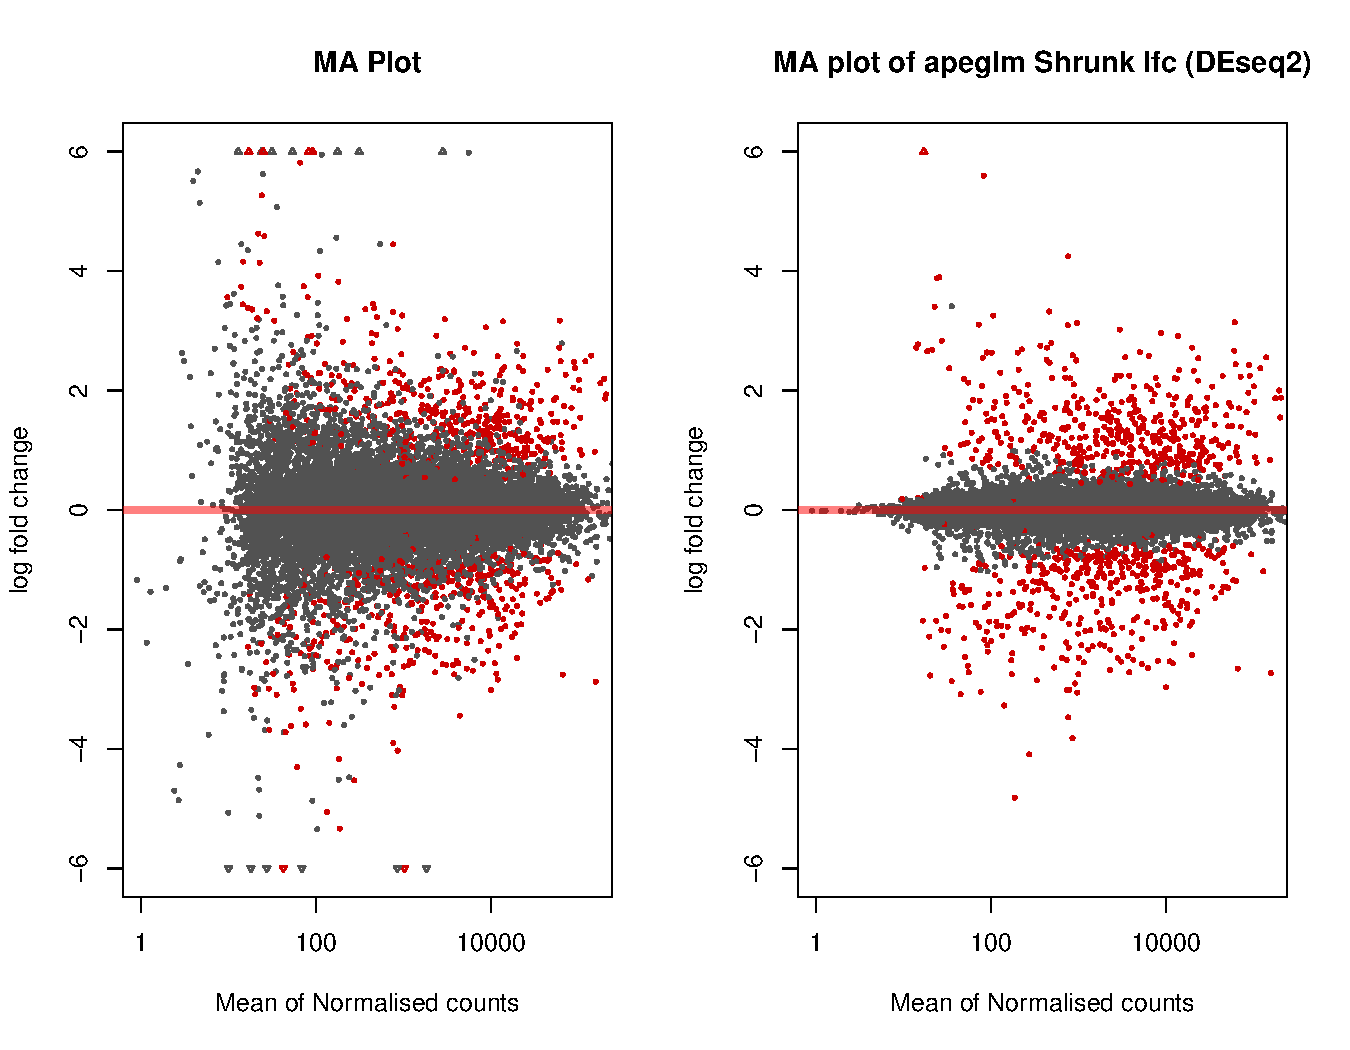
\includegraphics{Untitled_files/figure-latex/Deseq2-7.pdf}

\begin{Shaded}
\begin{Highlighting}[]
\NormalTok{res05_D4 <-}\StringTok{ }\KeywordTok{results}\NormalTok{(dds4, }\DataTypeTok{alpha=}\FloatTok{0.05}\NormalTok{)}
\KeywordTok{summary}\NormalTok{(res05_D4)}
\end{Highlighting}
\end{Shaded}

\begin{verbatim}
## 
## out of 12999 with nonzero total read count
## adjusted p-value < 0.05
## LFC > 0 (up)       : 394, 3%
## LFC < 0 (down)     : 369, 2.8%
## outliers [1]       : 95, 0.73%
## low counts [2]     : 0, 0%
## (mean count < 0)
## [1] see 'cooksCutoff' argument of ?results
## [2] see 'independentFiltering' argument of ?results
\end{verbatim}

\begin{Shaded}
\begin{Highlighting}[]
\KeywordTok{par}\NormalTok{(}\DataTypeTok{mfrow=}\KeywordTok{c}\NormalTok{(}\DecValTok{1}\NormalTok{,}\DecValTok{1}\NormalTok{))}
\KeywordTok{plotCounts}\NormalTok{(dds4, }\DataTypeTok{gene=}\KeywordTok{which.min}\NormalTok{(res4}\OperatorTok{$}\NormalTok{padj), }\DataTypeTok{intgroup=}\StringTok{"Groups"}\NormalTok{)}
\end{Highlighting}
\end{Shaded}

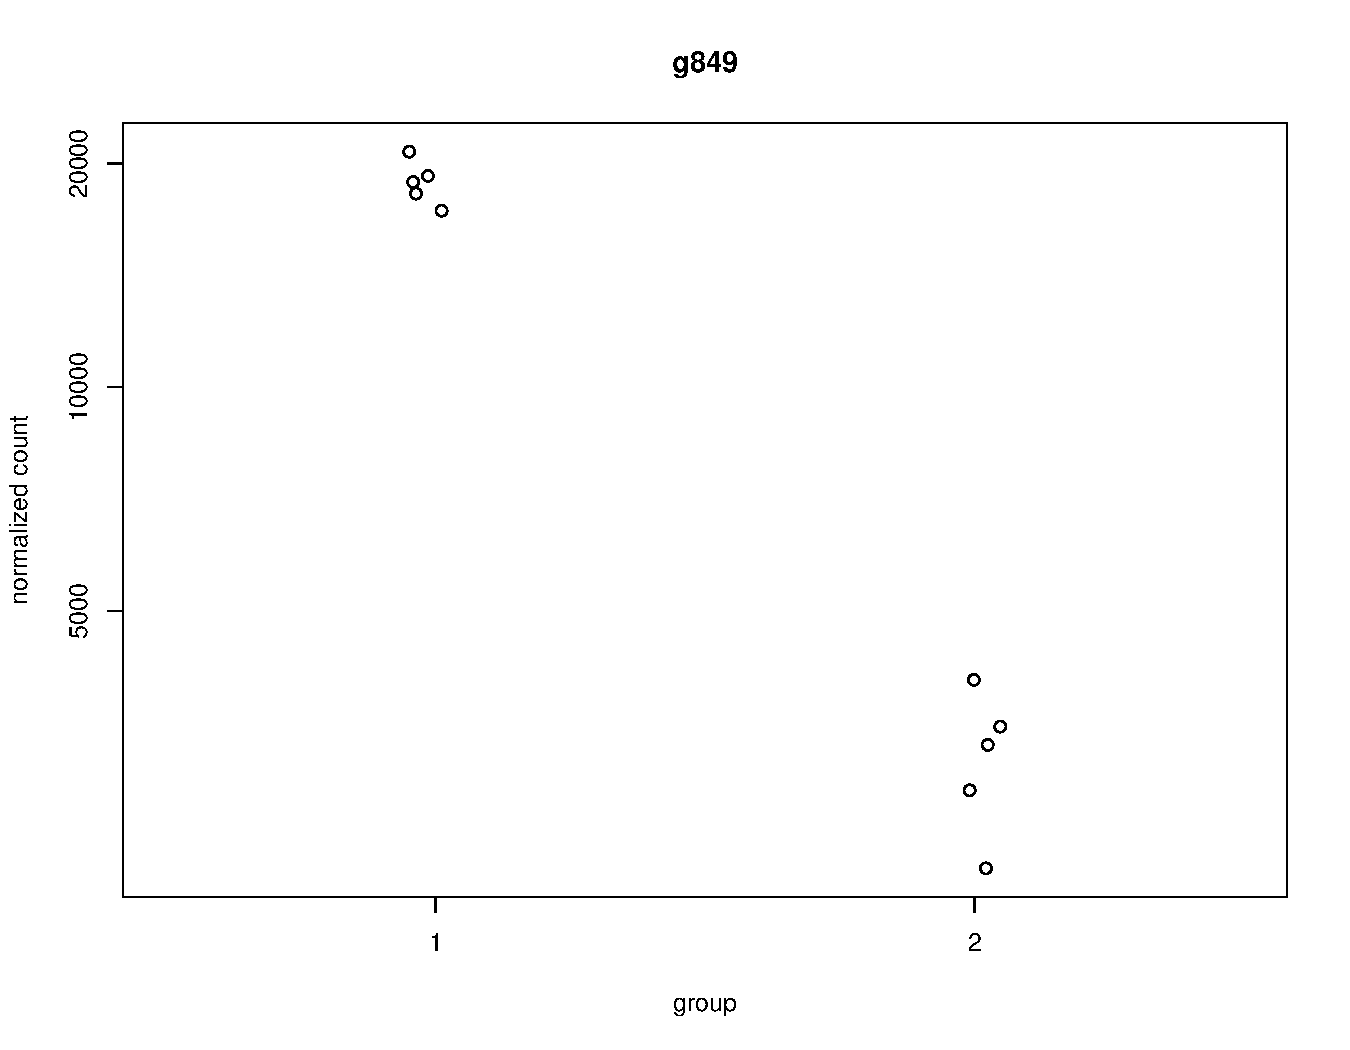
\includegraphics{Untitled_files/figure-latex/Deseq2-8.pdf}

\begin{Shaded}
\begin{Highlighting}[]
\NormalTok{resSig_D4 <-}\StringTok{ }\KeywordTok{subset}\NormalTok{(res05_D4, padj }\OperatorTok{<}\StringTok{ }\FloatTok{0.05}\NormalTok{)}
\KeywordTok{nrow}\NormalTok{(resSig_D4)}
\end{Highlighting}
\end{Shaded}

\begin{verbatim}
## [1] 763
\end{verbatim}

\begin{Shaded}
\begin{Highlighting}[]
\KeywordTok{write.csv}\NormalTok{(resSig_D4,}\StringTok{'DEseq2_D4_res.csv'}\NormalTok{)}

\KeywordTok{write.csv}\NormalTok{(}\KeywordTok{rownames}\NormalTok{(resSig_D1),}\StringTok{'DEseq2_T1.csv'}\NormalTok{)}
\KeywordTok{write.csv}\NormalTok{(}\KeywordTok{rownames}\NormalTok{(resSig_D2),}\StringTok{'DEseq2_T2.csv'}\NormalTok{)}
\KeywordTok{write.csv}\NormalTok{(}\KeywordTok{rownames}\NormalTok{(resSig_D3),}\StringTok{'DEseq2_T3.csv'}\NormalTok{)}
\KeywordTok{write.csv}\NormalTok{(}\KeywordTok{rownames}\NormalTok{(resSig_D4),}\StringTok{'DEseq2_T4.csv'}\NormalTok{)}
\end{Highlighting}
\end{Shaded}

\begin{Shaded}
\begin{Highlighting}[]
\KeywordTok{layout}\NormalTok{(}\KeywordTok{matrix}\NormalTok{(}\KeywordTok{c}\NormalTok{(}\DecValTok{1}\NormalTok{,}\DecValTok{2}\NormalTok{,}\DecValTok{3}\NormalTok{,}\DecValTok{4}\NormalTok{,}\DecValTok{5}\NormalTok{,}\DecValTok{6}\NormalTok{), }\DecValTok{3}\NormalTok{, }\DecValTok{2}\NormalTok{, }\DataTypeTok{byrow=}\OtherTok{TRUE}\NormalTok{))}
\KeywordTok{par}\NormalTok{(}\DataTypeTok{mfrow=}\KeywordTok{c}\NormalTok{(}\DecValTok{1}\NormalTok{,}\DecValTok{2}\NormalTok{),}\DataTypeTok{oma =} \KeywordTok{c}\NormalTok{(}\DecValTok{0}\NormalTok{, }\DecValTok{0}\NormalTok{, }\DecValTok{2}\NormalTok{, }\DecValTok{0}\NormalTok{))}

\CommentTok{#write the datasets into formats readable by readGeneExp}
\KeywordTok{write.table}\NormalTok{(D1}\OperatorTok{@}\NormalTok{count.matrix, }\DataTypeTok{file =} \StringTok{"D1.csv"}\NormalTok{)}
\KeywordTok{write.table}\NormalTok{(D2}\OperatorTok{@}\NormalTok{count.matrix, }\DataTypeTok{file =} \StringTok{"D2.csv"}\NormalTok{)}
\KeywordTok{write.table}\NormalTok{(D3}\OperatorTok{@}\NormalTok{count.matrix, }\DataTypeTok{file =} \StringTok{"D3.csv"}\NormalTok{)}
\KeywordTok{write.table}\NormalTok{(D4}\OperatorTok{@}\NormalTok{count.matrix, }\DataTypeTok{file =} \StringTok{"D4.csv"}\NormalTok{)}

\CommentTok{#Get a DEGseq object for both conditions(Groups)}
\NormalTok{geneExpMatrixD1_}\DecValTok{1}\NormalTok{ <-}\StringTok{ }\KeywordTok{readGeneExp}\NormalTok{(}\KeywordTok{here}\NormalTok{(}\StringTok{"Project"}\NormalTok{,}\StringTok{"D1.csv"}\NormalTok{), }\DataTypeTok{geneCol=}\DecValTok{1}\NormalTok{, }\DataTypeTok{valCol=}\KeywordTok{c}\NormalTok{(}\DecValTok{2}\NormalTok{,}\DecValTok{3}\NormalTok{,}\DecValTok{4}\NormalTok{,}\DecValTok{5}\NormalTok{))}
\NormalTok{geneExpMatrixD1_}\DecValTok{2}\NormalTok{ <-}\StringTok{ }\KeywordTok{readGeneExp}\NormalTok{(}\KeywordTok{here}\NormalTok{(}\StringTok{"Project"}\NormalTok{,}\StringTok{"D1.csv"}\NormalTok{), }\DataTypeTok{geneCol=}\DecValTok{1}\NormalTok{, }\DataTypeTok{valCol=}\KeywordTok{c}\NormalTok{(}\DecValTok{6}\NormalTok{,}\DecValTok{7}\NormalTok{,}\DecValTok{8}\NormalTok{,}\DecValTok{9}\NormalTok{))}

\NormalTok{geneExpMatrixD2_}\DecValTok{1}\NormalTok{ <-}\StringTok{ }\KeywordTok{readGeneExp}\NormalTok{(}\KeywordTok{here}\NormalTok{(}\StringTok{"Project"}\NormalTok{,}\StringTok{"D2.csv"}\NormalTok{), }\DataTypeTok{geneCol=}\DecValTok{1}\NormalTok{, }\DataTypeTok{valCol=}\KeywordTok{c}\NormalTok{(}\DecValTok{2}\NormalTok{,}\DecValTok{3}\NormalTok{,}\DecValTok{4}\NormalTok{,}\DecValTok{5}\NormalTok{))}
\NormalTok{geneExpMatrixD2_}\DecValTok{2}\NormalTok{ <-}\StringTok{ }\KeywordTok{readGeneExp}\NormalTok{(}\KeywordTok{here}\NormalTok{(}\StringTok{"Project"}\NormalTok{,}\StringTok{"D2.csv"}\NormalTok{), }\DataTypeTok{geneCol=}\DecValTok{1}\NormalTok{, }\DataTypeTok{valCol=}\KeywordTok{c}\NormalTok{(}\DecValTok{6}\NormalTok{,}\DecValTok{7}\NormalTok{,}\DecValTok{8}\NormalTok{,}\DecValTok{9}\NormalTok{))}

\NormalTok{geneExpMatrixD3_}\DecValTok{1}\NormalTok{ <-}\StringTok{ }\KeywordTok{readGeneExp}\NormalTok{(}\KeywordTok{here}\NormalTok{(}\StringTok{"Project"}\NormalTok{,}\StringTok{"D3.csv"}\NormalTok{), }\DataTypeTok{geneCol=}\DecValTok{1}\NormalTok{, }\DataTypeTok{valCol=}\KeywordTok{c}\NormalTok{(}\DecValTok{2}\NormalTok{,}\DecValTok{3}\NormalTok{,}\DecValTok{4}\NormalTok{,}\DecValTok{5}\NormalTok{))}
\NormalTok{geneExpMatrixD3_}\DecValTok{2}\NormalTok{ <-}\StringTok{ }\KeywordTok{readGeneExp}\NormalTok{(}\KeywordTok{here}\NormalTok{(}\StringTok{"Project"}\NormalTok{,}\StringTok{"D3.csv"}\NormalTok{), }\DataTypeTok{geneCol=}\DecValTok{1}\NormalTok{, }\DataTypeTok{valCol=}\KeywordTok{c}\NormalTok{(}\DecValTok{6}\NormalTok{,}\DecValTok{7}\NormalTok{,}\DecValTok{8}\NormalTok{,}\DecValTok{9}\NormalTok{))}

\NormalTok{geneExpMatrixD4_}\DecValTok{1}\NormalTok{ <-}\StringTok{ }\KeywordTok{readGeneExp}\NormalTok{(}\KeywordTok{here}\NormalTok{(}\StringTok{"Project"}\NormalTok{,}\StringTok{"D4.csv"}\NormalTok{), }\DataTypeTok{geneCol=}\DecValTok{1}\NormalTok{, }\DataTypeTok{valCol=}\KeywordTok{c}\NormalTok{(}\DecValTok{2}\NormalTok{,}\DecValTok{3}\NormalTok{,}\DecValTok{4}\NormalTok{,}\DecValTok{5}\NormalTok{))}
\NormalTok{geneExpMatrixD4_}\DecValTok{2}\NormalTok{ <-}\StringTok{ }\KeywordTok{readGeneExp}\NormalTok{(}\KeywordTok{here}\NormalTok{(}\StringTok{"Project"}\NormalTok{,}\StringTok{"D4.csv"}\NormalTok{), }\DataTypeTok{geneCol=}\DecValTok{1}\NormalTok{, }\DataTypeTok{valCol=}\KeywordTok{c}\NormalTok{(}\DecValTok{6}\NormalTok{,}\DecValTok{7}\NormalTok{,}\DecValTok{8}\NormalTok{,}\DecValTok{9}\NormalTok{))}


\CommentTok{#Run DEGseq for all the datasets and save the results of various object}
\NormalTok{DEGexp <-}\StringTok{ }\KeywordTok{DEGexp}\NormalTok{(}\DataTypeTok{geneExpMatrix1=}\NormalTok{ geneExpMatrixD1_}\DecValTok{1}\NormalTok{, }\DataTypeTok{groupLabel1=}\StringTok{"Group1"}\NormalTok{,}\DataTypeTok{depth1=} \FloatTok{1e7}\NormalTok{, }\DataTypeTok{depth2=}\FloatTok{1e7}\NormalTok{, }\DataTypeTok{geneExpMatrix2 =}\NormalTok{ geneExpMatrixD1_}\DecValTok{2}\NormalTok{ , }\DataTypeTok{groupLabel2=}\StringTok{"Group2"}\NormalTok{, }\DataTypeTok{thresholdKind=}\DecValTok{3}\NormalTok{, }\DataTypeTok{qValue =} \FloatTok{0.05}\NormalTok{, }\DataTypeTok{outputDir =} \KeywordTok{here}\NormalTok{(}\StringTok{"Project"}\NormalTok{,}\StringTok{"DEGseq_D1"}\NormalTok{))}
\end{Highlighting}
\end{Shaded}

\begin{verbatim}
## Please wait...
## gene id column in geneExpMatrix1 for sample1:  1 
## expression value column(s) in geneExpMatrix1: 2 
## total number of reads uniquely mapped to genome obtained from sample1: 1e+07 
## gene id column in geneExpMatrix2 for sample2:  1 
## expression value column(s) in geneExpMatrix2: 2 
## total number of reads uniquely mapped to genome obtained from sample2: 1e+07 
## 
## method to identify differentially expressed genes:  LRT 
## qValue threshold (Benjamini et al. 1995): 0.05 
## output directory: /Users/abdul-rahmanbukari/Documents/BIOSTATS/Project/DEGseq_D1 
## 
## Please wait ...
\end{verbatim}

\begin{verbatim}
## Identifying differentially expressed genes ...
## Please wait patiently ...
\end{verbatim}

\begin{verbatim}
## output ...
## 
## Done ...
## The results can be observed in directory:  /Users/abdul-rahmanbukari/Documents/BIOSTATS/Project/DEGseq_D1
\end{verbatim}

\begin{Shaded}
\begin{Highlighting}[]
\NormalTok{DEGseq_D1 <-}\StringTok{ }\KeywordTok{read.table}\NormalTok{(}\KeywordTok{here}\NormalTok{(}\StringTok{"Project"}\NormalTok{,}\StringTok{"DEGseq_D1"}\NormalTok{,}\StringTok{"output_score.txt"}\NormalTok{), }\DataTypeTok{header=}\OtherTok{TRUE}\NormalTok{)}
\NormalTok{DEGseq_D1_res <-}\StringTok{ }\KeywordTok{subset}\NormalTok{(DEGseq_D1, Signature.q.value.Benjamini.et.al..}\DecValTok{1995}\NormalTok{....}\DecValTok{0}\NormalTok{.}\FloatTok{05.} \OperatorTok{==}\OtherTok{TRUE}\NormalTok{)}
\KeywordTok{nrow}\NormalTok{(DEGseq_D1_res)}
\end{Highlighting}
\end{Shaded}

\begin{verbatim}
## [1] 10583
\end{verbatim}

\begin{Shaded}
\begin{Highlighting}[]
\KeywordTok{write.csv}\NormalTok{(DEGseq_D1_res,}\StringTok{'DEGseq_D1_res.csv'}\NormalTok{)}

\NormalTok{DEGexp <-}\StringTok{ }\KeywordTok{DEGexp}\NormalTok{(}\DataTypeTok{geneExpMatrix1=}\NormalTok{ geneExpMatrixD2_}\DecValTok{1}\NormalTok{, }\DataTypeTok{groupLabel1=}\StringTok{"Group1"}\NormalTok{, }\DataTypeTok{depth1=} \FloatTok{1e7}\NormalTok{, }\DataTypeTok{depth2=}\FloatTok{1e7}\NormalTok{, }\DataTypeTok{geneExpMatrix2 =}\NormalTok{ geneExpMatrixD2_}\DecValTok{2}\NormalTok{ , }\DataTypeTok{groupLabel2=}\StringTok{"Group2"}\NormalTok{, }\DataTypeTok{thresholdKind=}\DecValTok{3}\NormalTok{, }\DataTypeTok{qValue =} \FloatTok{0.05}\NormalTok{, }\DataTypeTok{outputDir =} \KeywordTok{here}\NormalTok{(}\StringTok{"Project"}\NormalTok{,}\StringTok{"DEGseq_D2"}\NormalTok{))}
\end{Highlighting}
\end{Shaded}

\begin{verbatim}
## Please wait...
## gene id column in geneExpMatrix1 for sample1:  1 
## expression value column(s) in geneExpMatrix1: 2 
## total number of reads uniquely mapped to genome obtained from sample1: 1e+07 
## gene id column in geneExpMatrix2 for sample2:  1 
## expression value column(s) in geneExpMatrix2: 2 
## total number of reads uniquely mapped to genome obtained from sample2: 1e+07 
## 
## method to identify differentially expressed genes:  LRT 
## qValue threshold (Benjamini et al. 1995): 0.05 
## output directory: /Users/abdul-rahmanbukari/Documents/BIOSTATS/Project/DEGseq_D2 
## 
## Please wait ...
\end{verbatim}

\begin{verbatim}
## Identifying differentially expressed genes ...
## Please wait patiently ...
\end{verbatim}

\begin{verbatim}
## output ...
## 
## Done ...
## The results can be observed in directory:  /Users/abdul-rahmanbukari/Documents/BIOSTATS/Project/DEGseq_D2
\end{verbatim}

\begin{Shaded}
\begin{Highlighting}[]
\NormalTok{DEGseq_D2 <-}\StringTok{ }\KeywordTok{read.table}\NormalTok{(}\KeywordTok{here}\NormalTok{(}\StringTok{"Project"}\NormalTok{,}\StringTok{"DEGseq_D2"}\NormalTok{,}\StringTok{"output_score.txt"}\NormalTok{), }\DataTypeTok{header=}\OtherTok{TRUE}\NormalTok{)}
\NormalTok{DEGseq_D2_res <-}\StringTok{ }\KeywordTok{subset}\NormalTok{(DEGseq_D2, Signature.q.value.Benjamini.et.al..}\DecValTok{1995}\NormalTok{....}\DecValTok{0}\NormalTok{.}\FloatTok{05.} \OperatorTok{==}\OtherTok{TRUE}\NormalTok{)}
\KeywordTok{nrow}\NormalTok{(DEGseq_D2_res)}
\end{Highlighting}
\end{Shaded}

\begin{verbatim}
## [1] 10917
\end{verbatim}

\begin{Shaded}
\begin{Highlighting}[]
\KeywordTok{write.csv}\NormalTok{(DEGseq_D2_res,}\StringTok{'DEGseq_D2_res.csv'}\NormalTok{)}

\NormalTok{DEGexp <-}\StringTok{ }\KeywordTok{DEGexp}\NormalTok{(}\DataTypeTok{geneExpMatrix1=}\NormalTok{ geneExpMatrixD3_}\DecValTok{1}\NormalTok{, }\DataTypeTok{groupLabel1=}\StringTok{"Group1"}\NormalTok{, }\DataTypeTok{depth1=} \FloatTok{1e7}\NormalTok{, }\DataTypeTok{depth2=}\FloatTok{1e7}\NormalTok{, }\DataTypeTok{geneExpMatrix2 =}\NormalTok{ geneExpMatrixD3_}\DecValTok{2}\NormalTok{ , }\DataTypeTok{groupLabel2=}\StringTok{"Group2"}\NormalTok{, }\DataTypeTok{thresholdKind=}\DecValTok{3}\NormalTok{, }\DataTypeTok{qValue =} \FloatTok{0.05}\NormalTok{, }\DataTypeTok{outputDir =} \KeywordTok{here}\NormalTok{(}\StringTok{"Project"}\NormalTok{,}\StringTok{"DEGseq_D3"}\NormalTok{))}
\end{Highlighting}
\end{Shaded}

\begin{verbatim}
## Please wait...
## gene id column in geneExpMatrix1 for sample1:  1 
## expression value column(s) in geneExpMatrix1: 2 
## total number of reads uniquely mapped to genome obtained from sample1: 1e+07 
## gene id column in geneExpMatrix2 for sample2:  1 
## expression value column(s) in geneExpMatrix2: 2 
## total number of reads uniquely mapped to genome obtained from sample2: 1e+07 
## 
## method to identify differentially expressed genes:  LRT 
## qValue threshold (Benjamini et al. 1995): 0.05 
## output directory: /Users/abdul-rahmanbukari/Documents/BIOSTATS/Project/DEGseq_D3 
## 
## Please wait ...
\end{verbatim}

\begin{verbatim}
## Identifying differentially expressed genes ...
## Please wait patiently ...
\end{verbatim}

\begin{verbatim}
## output ...
## 
## Done ...
## The results can be observed in directory:  /Users/abdul-rahmanbukari/Documents/BIOSTATS/Project/DEGseq_D3
\end{verbatim}

\begin{Shaded}
\begin{Highlighting}[]
\NormalTok{DEGseq_D3 <-}\StringTok{ }\KeywordTok{read.table}\NormalTok{(}\KeywordTok{here}\NormalTok{(}\StringTok{"Project"}\NormalTok{,}\StringTok{"DEGseq_D3"}\NormalTok{,}\StringTok{"output_score.txt"}\NormalTok{), }\DataTypeTok{header=}\OtherTok{TRUE}\NormalTok{)}
\NormalTok{DEGseq_D3_res <-}\StringTok{ }\KeywordTok{subset}\NormalTok{(DEGseq_D3, Signature.q.value.Benjamini.et.al..}\DecValTok{1995}\NormalTok{....}\DecValTok{0}\NormalTok{.}\FloatTok{05.} \OperatorTok{==}\OtherTok{TRUE}\NormalTok{)}
\KeywordTok{nrow}\NormalTok{(DEGseq_D3_res)}
\end{Highlighting}
\end{Shaded}

\begin{verbatim}
## [1] 10941
\end{verbatim}

\begin{Shaded}
\begin{Highlighting}[]
\KeywordTok{write.csv}\NormalTok{(DEGseq_D3_res,}\StringTok{'DEGseq_D3_res.csv'}\NormalTok{)}

\NormalTok{DEGexp <-}\StringTok{ }\KeywordTok{DEGexp}\NormalTok{(}\DataTypeTok{geneExpMatrix1=}\NormalTok{ geneExpMatrixD4_}\DecValTok{1}\NormalTok{, }\DataTypeTok{groupLabel1=}\StringTok{"Group1"}\NormalTok{, }\DataTypeTok{depth1=} \FloatTok{1e7}\NormalTok{, }\DataTypeTok{depth2=}\FloatTok{1e7}\NormalTok{, }\DataTypeTok{geneExpMatrix2 =}\NormalTok{ geneExpMatrixD4_}\DecValTok{2}\NormalTok{ , }\DataTypeTok{groupLabel2=}\StringTok{"Group2"}\NormalTok{, }\DataTypeTok{thresholdKind=}\DecValTok{3}\NormalTok{, }\DataTypeTok{qValue =} \FloatTok{0.05}\NormalTok{, }\DataTypeTok{outputDir =} \KeywordTok{here}\NormalTok{(}\StringTok{"Project"}\NormalTok{,}\StringTok{"DEGseq_D4"}\NormalTok{))}
\end{Highlighting}
\end{Shaded}

\begin{verbatim}
## Please wait...
## gene id column in geneExpMatrix1 for sample1:  1 
## expression value column(s) in geneExpMatrix1: 2 
## total number of reads uniquely mapped to genome obtained from sample1: 1e+07 
## gene id column in geneExpMatrix2 for sample2:  1 
## expression value column(s) in geneExpMatrix2: 2 
## total number of reads uniquely mapped to genome obtained from sample2: 1e+07 
## 
## method to identify differentially expressed genes:  LRT 
## qValue threshold (Benjamini et al. 1995): 0.05 
## output directory: /Users/abdul-rahmanbukari/Documents/BIOSTATS/Project/DEGseq_D4 
## 
## Please wait ...
\end{verbatim}

\begin{verbatim}
## Identifying differentially expressed genes ...
## Please wait patiently ...
\end{verbatim}

\begin{verbatim}
## output ...
## 
## Done ...
## The results can be observed in directory:  /Users/abdul-rahmanbukari/Documents/BIOSTATS/Project/DEGseq_D4
\end{verbatim}

\begin{Shaded}
\begin{Highlighting}[]
\NormalTok{DEGseq_D4 <-}\StringTok{ }\KeywordTok{read.table}\NormalTok{(}\KeywordTok{here}\NormalTok{(}\StringTok{"Project"}\NormalTok{,}\StringTok{"DEGseq_D4"}\NormalTok{,}\StringTok{"output_score.txt"}\NormalTok{), }\DataTypeTok{header=}\OtherTok{TRUE}\NormalTok{)}
\NormalTok{DEGseq_D4_res <-}\StringTok{ }\KeywordTok{subset}\NormalTok{(DEGseq_D4, Signature.q.value.Benjamini.et.al..}\DecValTok{1995}\NormalTok{....}\DecValTok{0}\NormalTok{.}\FloatTok{05.} \OperatorTok{==}\OtherTok{TRUE}\NormalTok{)}
\KeywordTok{nrow}\NormalTok{(DEGseq_D4_res)}
\end{Highlighting}
\end{Shaded}

\begin{verbatim}
## [1] 10885
\end{verbatim}

\begin{Shaded}
\begin{Highlighting}[]
\KeywordTok{write.csv}\NormalTok{(DEGseq_D4_res,}\StringTok{'DEGseq_D4_res.csv'}\NormalTok{)}

\KeywordTok{View}\NormalTok{(DEGseq_D4)}
\KeywordTok{write.csv}\NormalTok{(DEGseq_D1_res}\OperatorTok{$}\NormalTok{GeneNames,}\DataTypeTok{row.names =}\OtherTok{FALSE}\NormalTok{, }\DataTypeTok{col.names =} \OtherTok{NA}\NormalTok{ ,}\StringTok{'DEGseq_T1.csv'}\NormalTok{)}
\end{Highlighting}
\end{Shaded}

\begin{verbatim}
## Warning in write.csv(DEGseq_D1_res$GeneNames, row.names = FALSE, col.names =
## NA, : attempt to set 'col.names' ignored
\end{verbatim}

\begin{Shaded}
\begin{Highlighting}[]
\KeywordTok{write.csv}\NormalTok{(DEGseq_D2_res}\OperatorTok{$}\NormalTok{GeneNames,}\DataTypeTok{row.names =}\OtherTok{FALSE}\NormalTok{, }\DataTypeTok{col.names =} \OtherTok{NA}\NormalTok{ ,}\StringTok{'DEGseq_T2.csv'}\NormalTok{)}
\end{Highlighting}
\end{Shaded}

\begin{verbatim}
## Warning in write.csv(DEGseq_D2_res$GeneNames, row.names = FALSE, col.names =
## NA, : attempt to set 'col.names' ignored
\end{verbatim}

\begin{Shaded}
\begin{Highlighting}[]
\KeywordTok{write.csv}\NormalTok{(DEGseq_D3_res}\OperatorTok{$}\NormalTok{GeneNames,}\DataTypeTok{row.names =}\OtherTok{FALSE}\NormalTok{, }\DataTypeTok{col.names =} \OtherTok{NA}\NormalTok{ ,}\StringTok{'DEGseq_T3.csv'}\NormalTok{)}
\end{Highlighting}
\end{Shaded}

\begin{verbatim}
## Warning in write.csv(DEGseq_D3_res$GeneNames, row.names = FALSE, col.names =
## NA, : attempt to set 'col.names' ignored
\end{verbatim}

\begin{Shaded}
\begin{Highlighting}[]
\KeywordTok{write.csv}\NormalTok{(DEGseq_D4_res}\OperatorTok{$}\NormalTok{GeneNames,}\DataTypeTok{row.names =}\OtherTok{FALSE}\NormalTok{, }\DataTypeTok{col.names =} \OtherTok{NA}\NormalTok{ ,}\StringTok{'DEGseq_T4.csv'}\NormalTok{)}
\end{Highlighting}
\end{Shaded}

\begin{verbatim}
## Warning in write.csv(DEGseq_D4_res$GeneNames, row.names = FALSE, col.names =
## NA, : attempt to set 'col.names' ignored
\end{verbatim}

\begin{Shaded}
\begin{Highlighting}[]
\CommentTok{#Generate Noiseq input objects with defined metadata}
\KeywordTok{write.table}\NormalTok{(Metadata, }\DataTypeTok{file =} \StringTok{"Metadata.csv"}\NormalTok{)}
\NormalTok{NoiseqD1 <-}\StringTok{ }\KeywordTok{readData}\NormalTok{(}\DataTypeTok{data=}\NormalTok{D1}\OperatorTok{@}\NormalTok{count.matrix, }\DataTypeTok{factors =} \KeywordTok{read.table}\NormalTok{(}\KeywordTok{here}\NormalTok{(}\StringTok{"Project"}\NormalTok{,}\StringTok{"Metadata.csv"}\NormalTok{)))}
\NormalTok{NoiseqD2 <-}\StringTok{ }\KeywordTok{readData}\NormalTok{(}\DataTypeTok{data=}\NormalTok{D2}\OperatorTok{@}\NormalTok{count.matrix, }\DataTypeTok{factors =} \KeywordTok{read.table}\NormalTok{(}\KeywordTok{here}\NormalTok{(}\StringTok{"Project"}\NormalTok{,}\StringTok{"Metadata.csv"}\NormalTok{)))}
\NormalTok{NoiseqD3 <-}\StringTok{ }\KeywordTok{readData}\NormalTok{(}\DataTypeTok{data=}\NormalTok{D3}\OperatorTok{@}\NormalTok{count.matrix, }\DataTypeTok{factors =} \KeywordTok{read.table}\NormalTok{(}\KeywordTok{here}\NormalTok{(}\StringTok{"Project"}\NormalTok{,}\StringTok{"Metadata.csv"}\NormalTok{)))}
\NormalTok{NoiseqD4 <-}\StringTok{ }\KeywordTok{readData}\NormalTok{(}\DataTypeTok{data=}\NormalTok{D4}\OperatorTok{@}\NormalTok{count.matrix, }\DataTypeTok{factors =} \KeywordTok{read.table}\NormalTok{(}\KeywordTok{here}\NormalTok{(}\StringTok{"Project"}\NormalTok{,}\StringTok{"Metadata.csv"}\NormalTok{)))}

\CommentTok{#run noiseq, obtain DEG and generate a plot }
\NormalTok{mynoiseq_D1 =}\StringTok{ }\KeywordTok{noiseq}\NormalTok{(NoiseqD1,}\DataTypeTok{norm=}\StringTok{"tmm"}\NormalTok{,}\DataTypeTok{factor =} \StringTok{"Groups"}\NormalTok{)}
\end{Highlighting}
\end{Shaded}

\begin{verbatim}
## [1] "Computing (M,D) values..."
## [1] "Computing probability of differential expression..."
\end{verbatim}

\begin{Shaded}
\begin{Highlighting}[]
\NormalTok{NoiseqD1_res <-}\StringTok{ }\KeywordTok{degenes}\NormalTok{(mynoiseq_D1, }\DataTypeTok{q =} \FloatTok{0.80}\NormalTok{, }\DataTypeTok{M =} \OtherTok{NULL}\NormalTok{)}
\end{Highlighting}
\end{Shaded}

\begin{verbatim}
## [1] "233 differentially expressed features"
\end{verbatim}

\begin{Shaded}
\begin{Highlighting}[]
\KeywordTok{write.csv}\NormalTok{(NoiseqD1_res,}\StringTok{'NoiseqD1_res.csv'}\NormalTok{)}
\KeywordTok{DE.plot}\NormalTok{(mynoiseq_D1, }\DataTypeTok{q =} \FloatTok{0.8}\NormalTok{, }\DataTypeTok{graphic =} \StringTok{"MD"}\NormalTok{, }\DataTypeTok{main=}\StringTok{"mynoiseq_D1"}\NormalTok{)}
\end{Highlighting}
\end{Shaded}

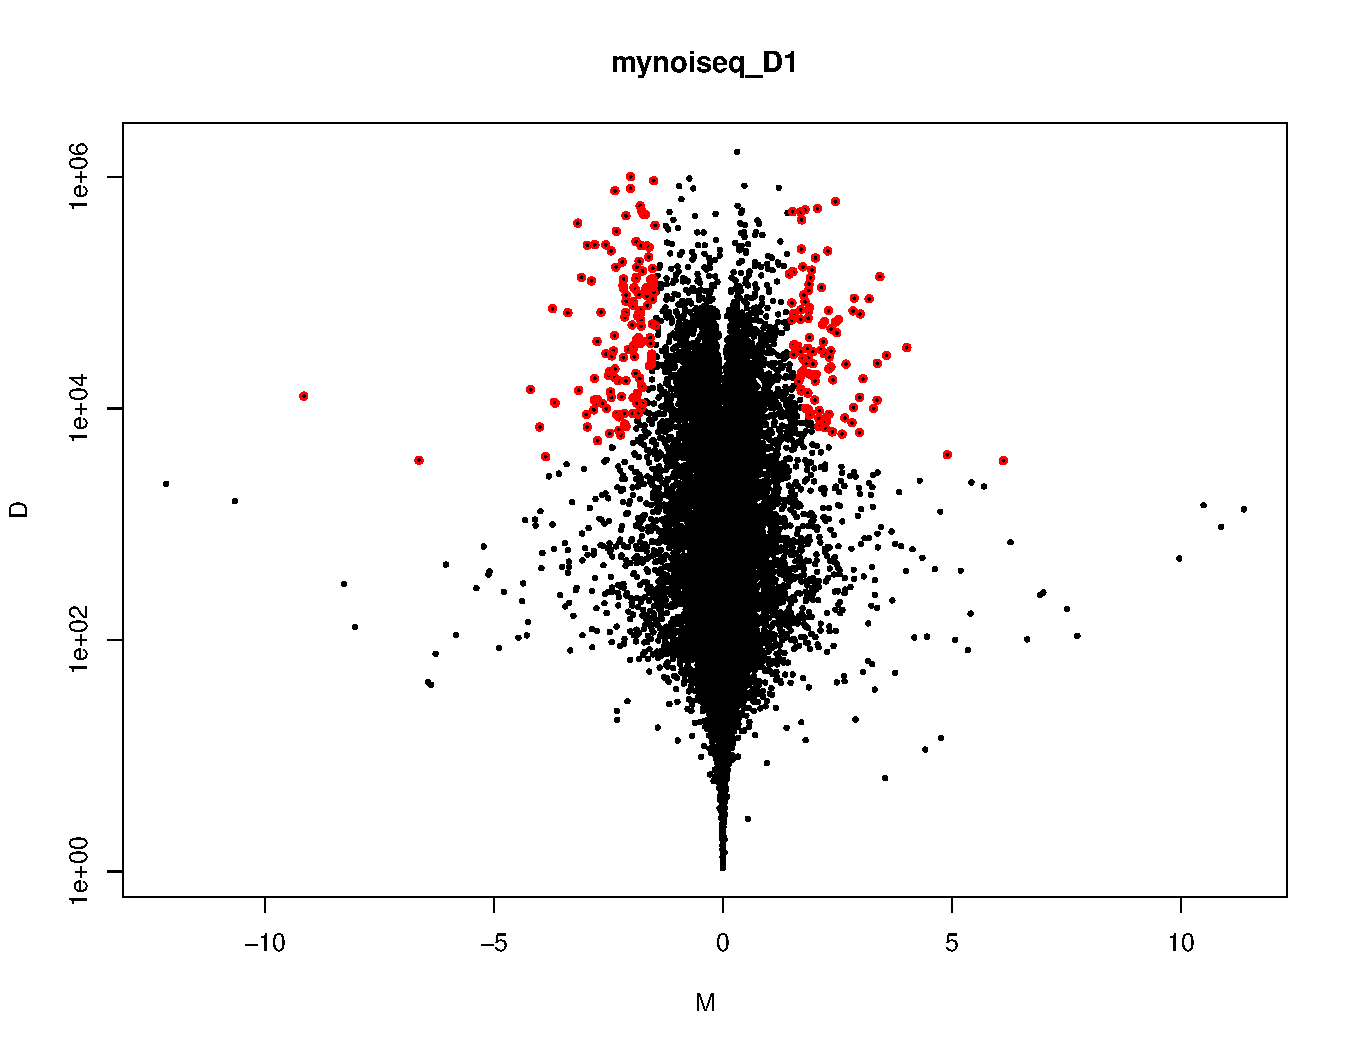
\includegraphics{Untitled_files/figure-latex/NOISeq-1.pdf}

\begin{verbatim}
## [1] "233 differentially expressed features"
\end{verbatim}

\begin{Shaded}
\begin{Highlighting}[]
\NormalTok{mynoiseq_D2 =}\StringTok{ }\KeywordTok{noiseq}\NormalTok{(NoiseqD2,}\DataTypeTok{factor =} \StringTok{"Groups"}\NormalTok{,}\DataTypeTok{norm=}\StringTok{"tmm"}\NormalTok{)}
\end{Highlighting}
\end{Shaded}

\begin{verbatim}
## [1] "Computing (M,D) values..."
## [1] "Computing probability of differential expression..."
\end{verbatim}

\begin{Shaded}
\begin{Highlighting}[]
\NormalTok{NoiseqD2_res <-}\StringTok{ }\KeywordTok{degenes}\NormalTok{(mynoiseq_D2, }\DataTypeTok{q =} \FloatTok{0.80}\NormalTok{, }\DataTypeTok{M =} \OtherTok{NULL}\NormalTok{)}
\end{Highlighting}
\end{Shaded}

\begin{verbatim}
## [1] "252 differentially expressed features"
\end{verbatim}

\begin{Shaded}
\begin{Highlighting}[]
\KeywordTok{write.csv}\NormalTok{(NoiseqD2_res,}\StringTok{'NoiseqD2_res.csv'}\NormalTok{)}
\KeywordTok{DE.plot}\NormalTok{(mynoiseq_D2, }\DataTypeTok{q =} \FloatTok{0.8}\NormalTok{, }\DataTypeTok{graphic =} \StringTok{"MD"}\NormalTok{, }\DataTypeTok{main=}\StringTok{"mynoiseq_D2"}\NormalTok{)}
\end{Highlighting}
\end{Shaded}

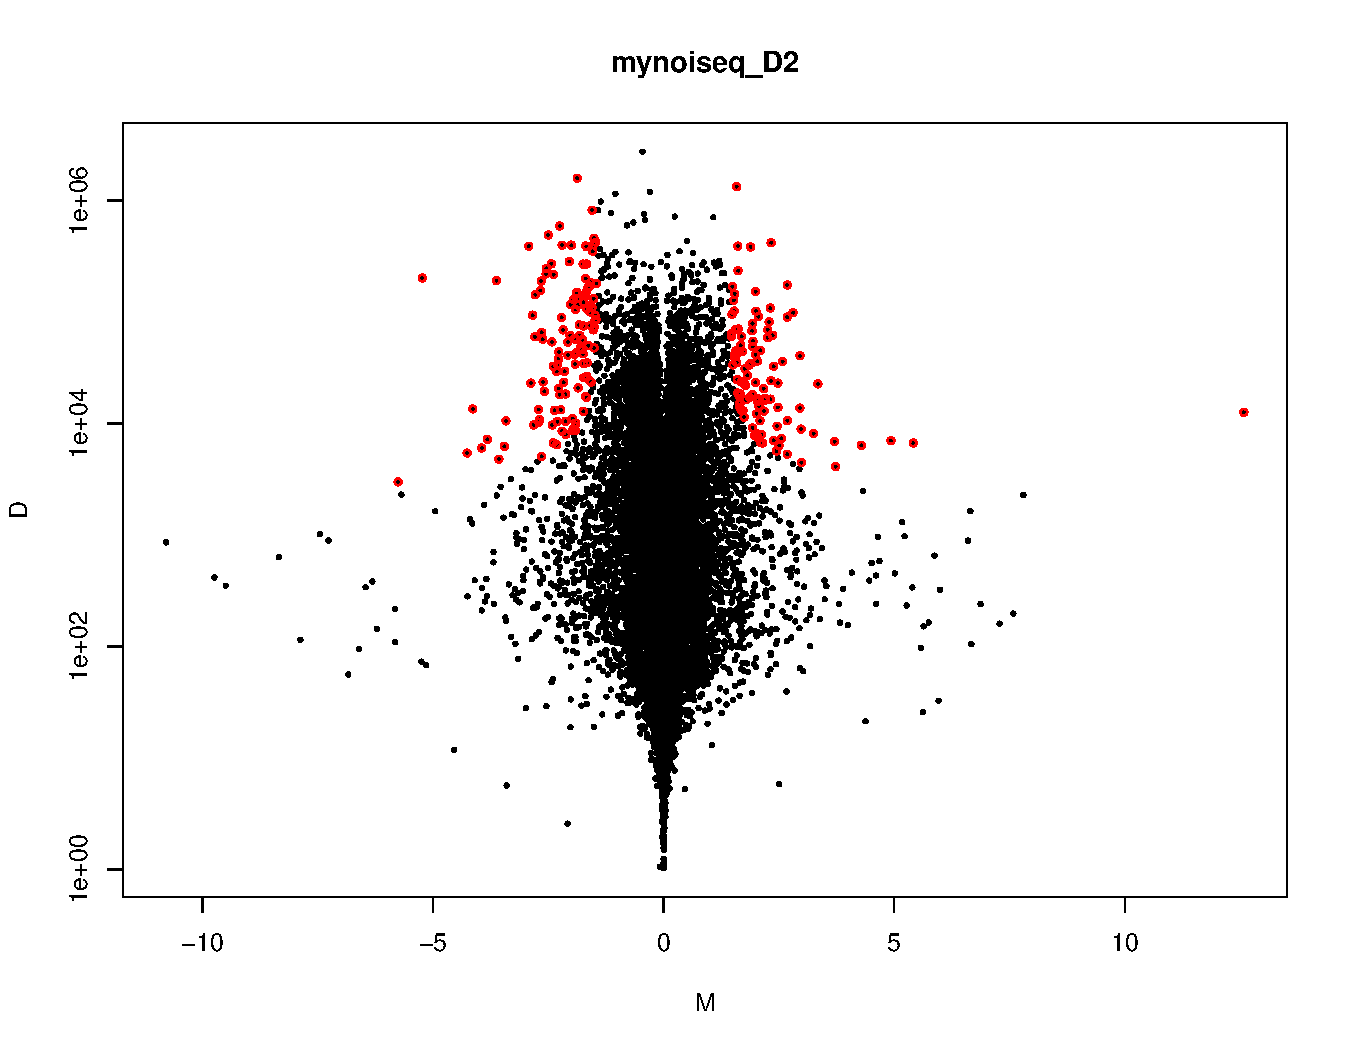
\includegraphics{Untitled_files/figure-latex/NOISeq-2.pdf}

\begin{verbatim}
## [1] "252 differentially expressed features"
\end{verbatim}

\begin{Shaded}
\begin{Highlighting}[]
\NormalTok{mynoiseq_D3 =}\StringTok{ }\KeywordTok{noiseq}\NormalTok{(NoiseqD3,}\DataTypeTok{factor =} \StringTok{"Groups"}\NormalTok{,}\DataTypeTok{norm=}\StringTok{"tmm"}\NormalTok{)}
\end{Highlighting}
\end{Shaded}

\begin{verbatim}
## [1] "Computing (M,D) values..."
## [1] "Computing probability of differential expression..."
\end{verbatim}

\begin{Shaded}
\begin{Highlighting}[]
\NormalTok{NoiseqD3_res <-}\StringTok{ }\KeywordTok{degenes}\NormalTok{(mynoiseq_D3, }\DataTypeTok{q =} \FloatTok{0.80}\NormalTok{, }\DataTypeTok{M =} \OtherTok{NULL}\NormalTok{)}
\end{Highlighting}
\end{Shaded}

\begin{verbatim}
## [1] "267 differentially expressed features"
\end{verbatim}

\begin{Shaded}
\begin{Highlighting}[]
\KeywordTok{write.csv}\NormalTok{(NoiseqD3_res,}\StringTok{'NoiseqD3_res.csv'}\NormalTok{)}
\KeywordTok{DE.plot}\NormalTok{(mynoiseq_D3, }\DataTypeTok{q =} \FloatTok{0.8}\NormalTok{, }\DataTypeTok{graphic =} \StringTok{"MD"}\NormalTok{, }\DataTypeTok{main=}\StringTok{"mynoiseq_D3"}\NormalTok{)}
\end{Highlighting}
\end{Shaded}

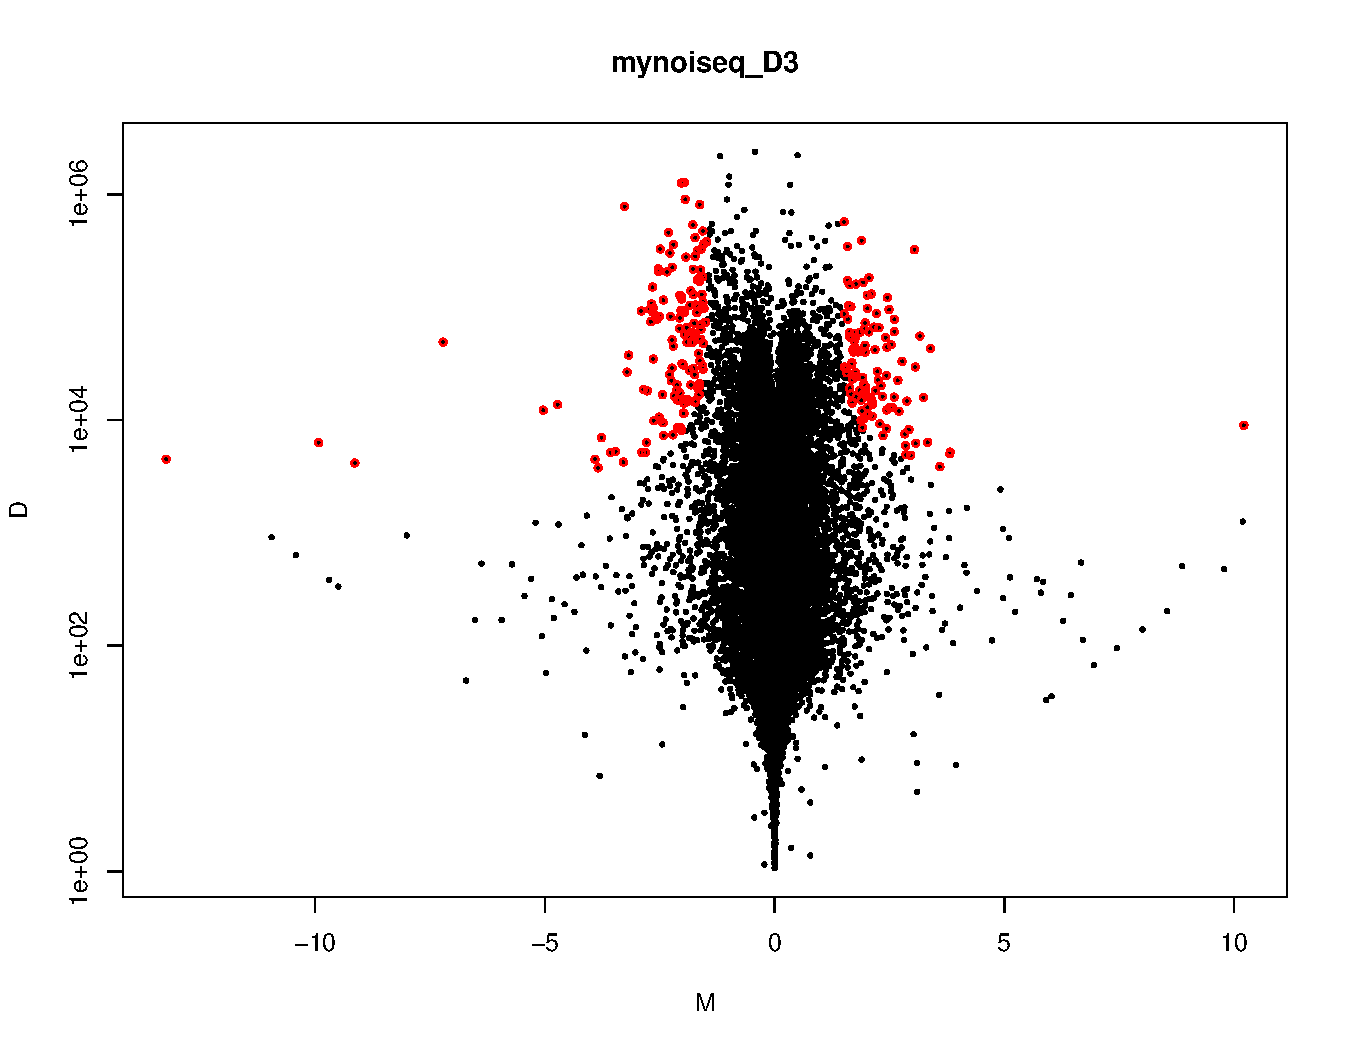
\includegraphics{Untitled_files/figure-latex/NOISeq-3.pdf}

\begin{verbatim}
## [1] "267 differentially expressed features"
\end{verbatim}

\begin{Shaded}
\begin{Highlighting}[]
\NormalTok{mynoiseq_D4 =}\StringTok{ }\KeywordTok{noiseq}\NormalTok{(NoiseqD4,}\DataTypeTok{factor =} \StringTok{"Groups"}\NormalTok{,}\DataTypeTok{norm=}\StringTok{"tmm"}\NormalTok{)}
\end{Highlighting}
\end{Shaded}

\begin{verbatim}
## [1] "Computing (M,D) values..."
## [1] "Computing probability of differential expression..."
\end{verbatim}

\begin{Shaded}
\begin{Highlighting}[]
\NormalTok{NoiseqD4_res <-}\StringTok{ }\KeywordTok{degenes}\NormalTok{(mynoiseq_D4, }\DataTypeTok{q =} \FloatTok{0.80}\NormalTok{, }\DataTypeTok{M =} \OtherTok{NULL}\NormalTok{)}
\end{Highlighting}
\end{Shaded}

\begin{verbatim}
## [1] "254 differentially expressed features"
\end{verbatim}

\begin{Shaded}
\begin{Highlighting}[]
\KeywordTok{write.csv}\NormalTok{(NoiseqD4_res,}\StringTok{'NoiseqD4_res.csv'}\NormalTok{)}
\KeywordTok{DE.plot}\NormalTok{(mynoiseq_D4, }\DataTypeTok{q =} \FloatTok{0.8}\NormalTok{, }\DataTypeTok{graphic =} \StringTok{"MD"}\NormalTok{, }\DataTypeTok{main=}\StringTok{"NOISeq_D4"}\NormalTok{)}
\end{Highlighting}
\end{Shaded}

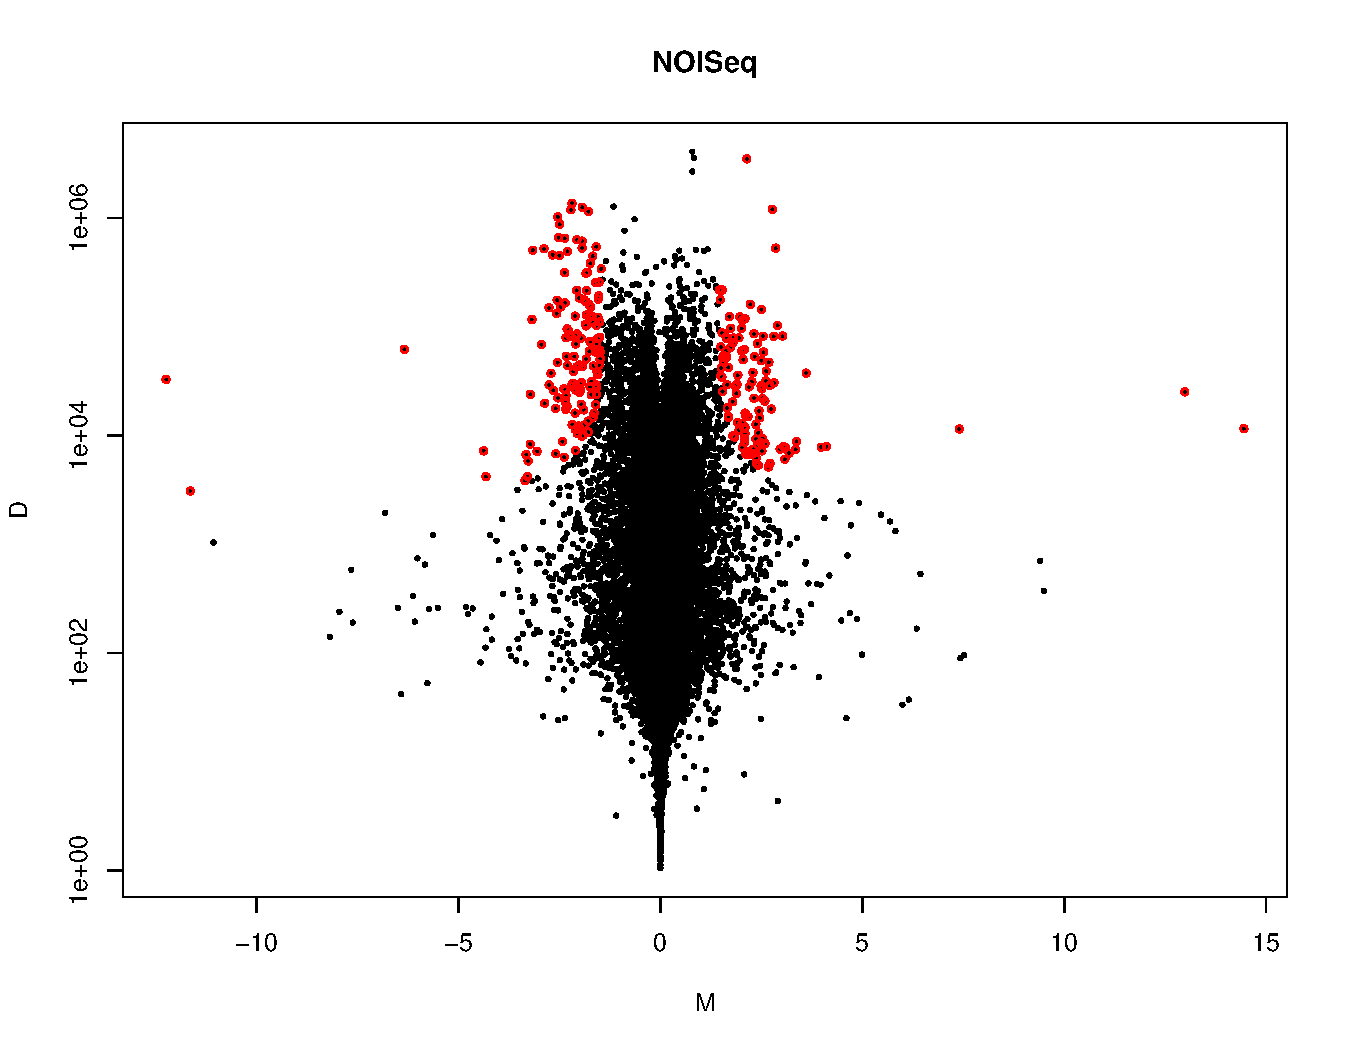
\includegraphics{Untitled_files/figure-latex/NOISeq-4.pdf}

\begin{verbatim}
## [1] "254 differentially expressed features"
\end{verbatim}

\begin{Shaded}
\begin{Highlighting}[]
\KeywordTok{nrow}\NormalTok{(NoiseqD1_res)}
\end{Highlighting}
\end{Shaded}

\begin{verbatim}
## [1] 233
\end{verbatim}

\begin{Shaded}
\begin{Highlighting}[]
\KeywordTok{nrow}\NormalTok{(NoiseqD2_res)}
\end{Highlighting}
\end{Shaded}

\begin{verbatim}
## [1] 252
\end{verbatim}

\begin{Shaded}
\begin{Highlighting}[]
\KeywordTok{nrow}\NormalTok{(NoiseqD3_res)}
\end{Highlighting}
\end{Shaded}

\begin{verbatim}
## [1] 267
\end{verbatim}

\begin{Shaded}
\begin{Highlighting}[]
\KeywordTok{nrow}\NormalTok{(NoiseqD4_res)}
\end{Highlighting}
\end{Shaded}

\begin{verbatim}
## [1] 254
\end{verbatim}

\begin{Shaded}
\begin{Highlighting}[]
\KeywordTok{write.csv}\NormalTok{(}\KeywordTok{rownames}\NormalTok{(NoiseqD1_res),}\StringTok{'NoiseqD1_T1.csv'}\NormalTok{)}
\KeywordTok{write.csv}\NormalTok{(}\KeywordTok{rownames}\NormalTok{(NoiseqD2_res),}\StringTok{'NoiseqD1_T2.csv'}\NormalTok{)}
\KeywordTok{write.csv}\NormalTok{(}\KeywordTok{rownames}\NormalTok{(NoiseqD3_res),}\StringTok{'NoiseqD1_T3.csv'}\NormalTok{)}
\KeywordTok{write.csv}\NormalTok{(}\KeywordTok{rownames}\NormalTok{(NoiseqD4_res),}\StringTok{'NoiseqD1_T4.csv'}\NormalTok{)}
\end{Highlighting}
\end{Shaded}

\hypertarget{results}{%
\subsection{Results}\label{results}}

The simulated reads depicted the characteristic distribution observed of
RNA-seq count data.

\hypertarget{performance-meassures}{%
\subsection{Performance meassures}\label{performance-meassures}}

The performance of the tools were based on three measures; Prescision,
Recall (specificity) and F1-score.

\(Prescision= \frac{True Postive}{True Positives + False Positives}\)

\(Recall= \frac{True Postive}{True Positives + False Negatives}\)

\(F1 Score = 2*\frac{Recall * Precision}{Recall + Precision}\)

Overall, DEseq2 producded the best performance (F1-score) with a good
levareage between prescision and recall (specificity). DEGseq recorded
the highest recall with the least prescision. The high fasle positive
calls by DEGseq is responsible for the degraded prescision and
subsequently the least F1-score. Although NOISeq was equally presice as
DEseq2, the poor recall lead to a degraded F1-score.

\begin{Shaded}
\begin{Highlighting}[]
\KeywordTok{par}\NormalTok{(}\DataTypeTok{mfrow=}\KeywordTok{c}\NormalTok{(}\DecValTok{2}\NormalTok{,}\DecValTok{2}\NormalTok{))}
\NormalTok{knitr}\OperatorTok{::}\KeywordTok{include_graphics}\NormalTok{(}\KeywordTok{c}\NormalTok{(}\KeywordTok{here}\NormalTok{(}\StringTok{"Project"}\NormalTok{,}\StringTok{"D1venn_result.png"}\NormalTok{),}\KeywordTok{here}\NormalTok{(}\StringTok{"Project"}\NormalTok{,}\StringTok{"D2venn_result.png"}\NormalTok{),}\KeywordTok{here}\NormalTok{(}\StringTok{"Project"}\NormalTok{,}\StringTok{"D3venn_result.png"}\NormalTok{),}\KeywordTok{here}\NormalTok{(}\StringTok{"Project"}\NormalTok{,}\StringTok{"D4venn_result.png"}\NormalTok{)))}
\end{Highlighting}
\end{Shaded}

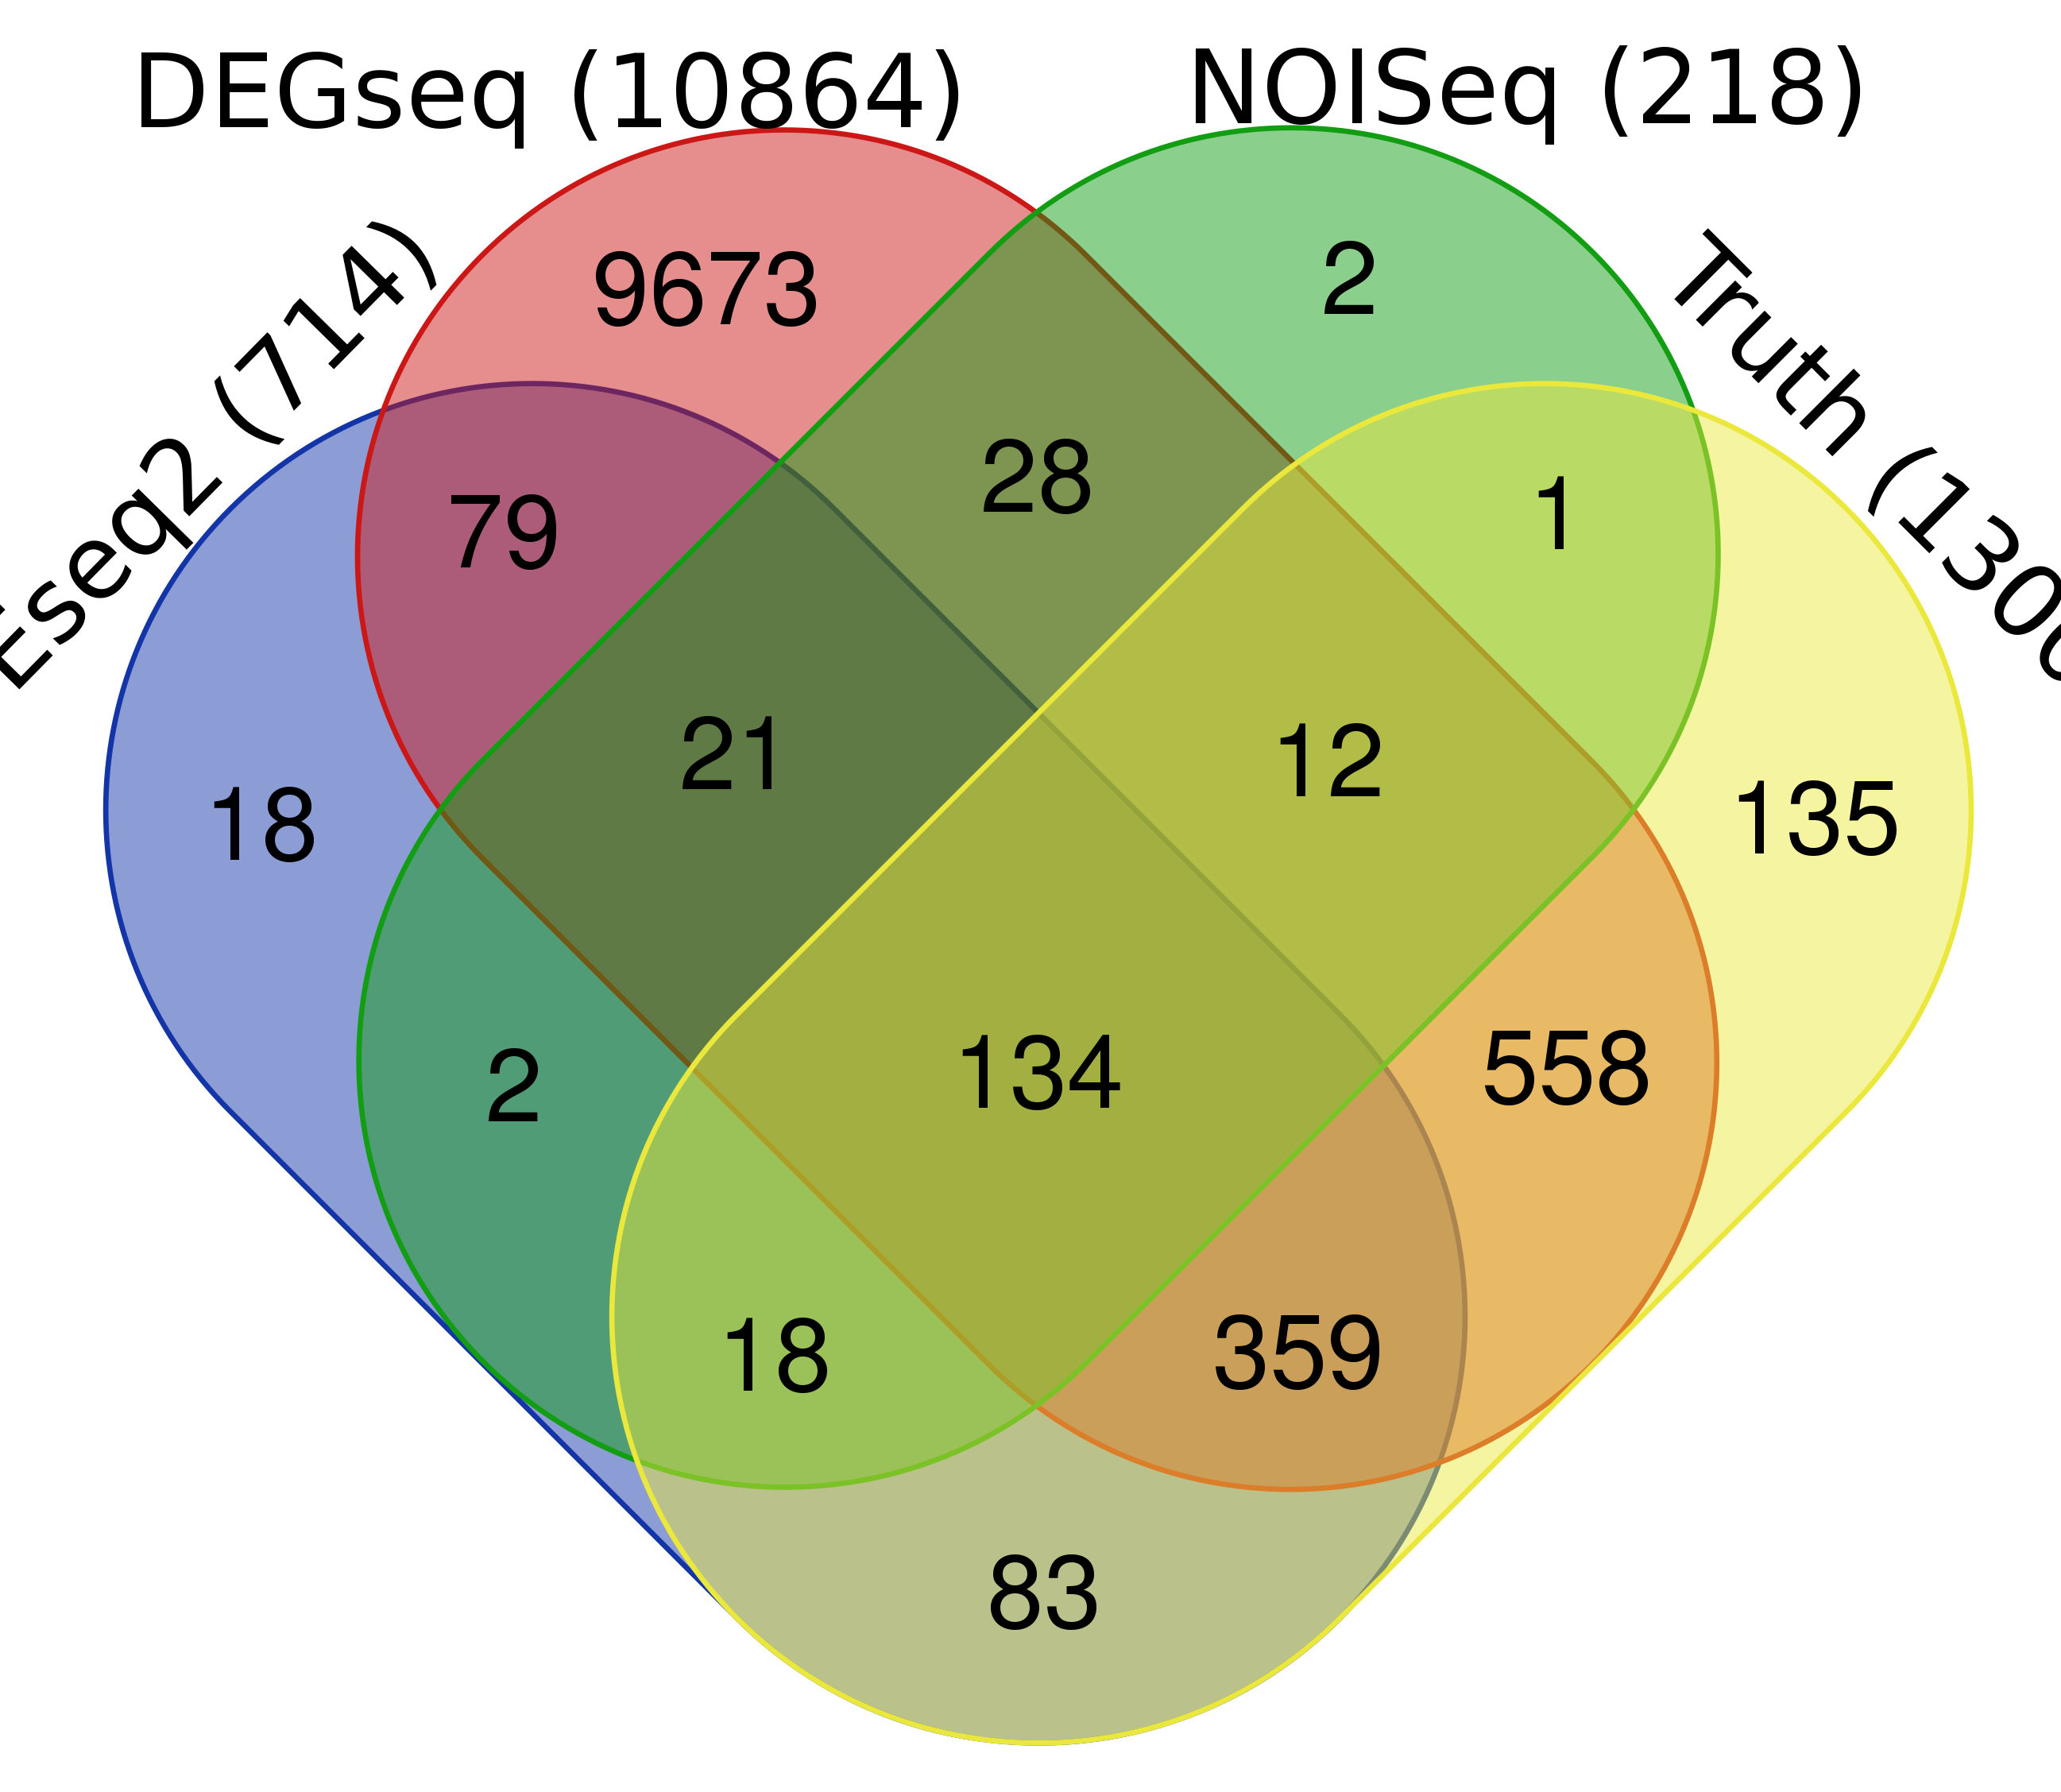
\includegraphics[width=0.33\linewidth]{/Users/abdul-rahmanbukari/Documents/BIOSTATS/Project/D1venn_result}
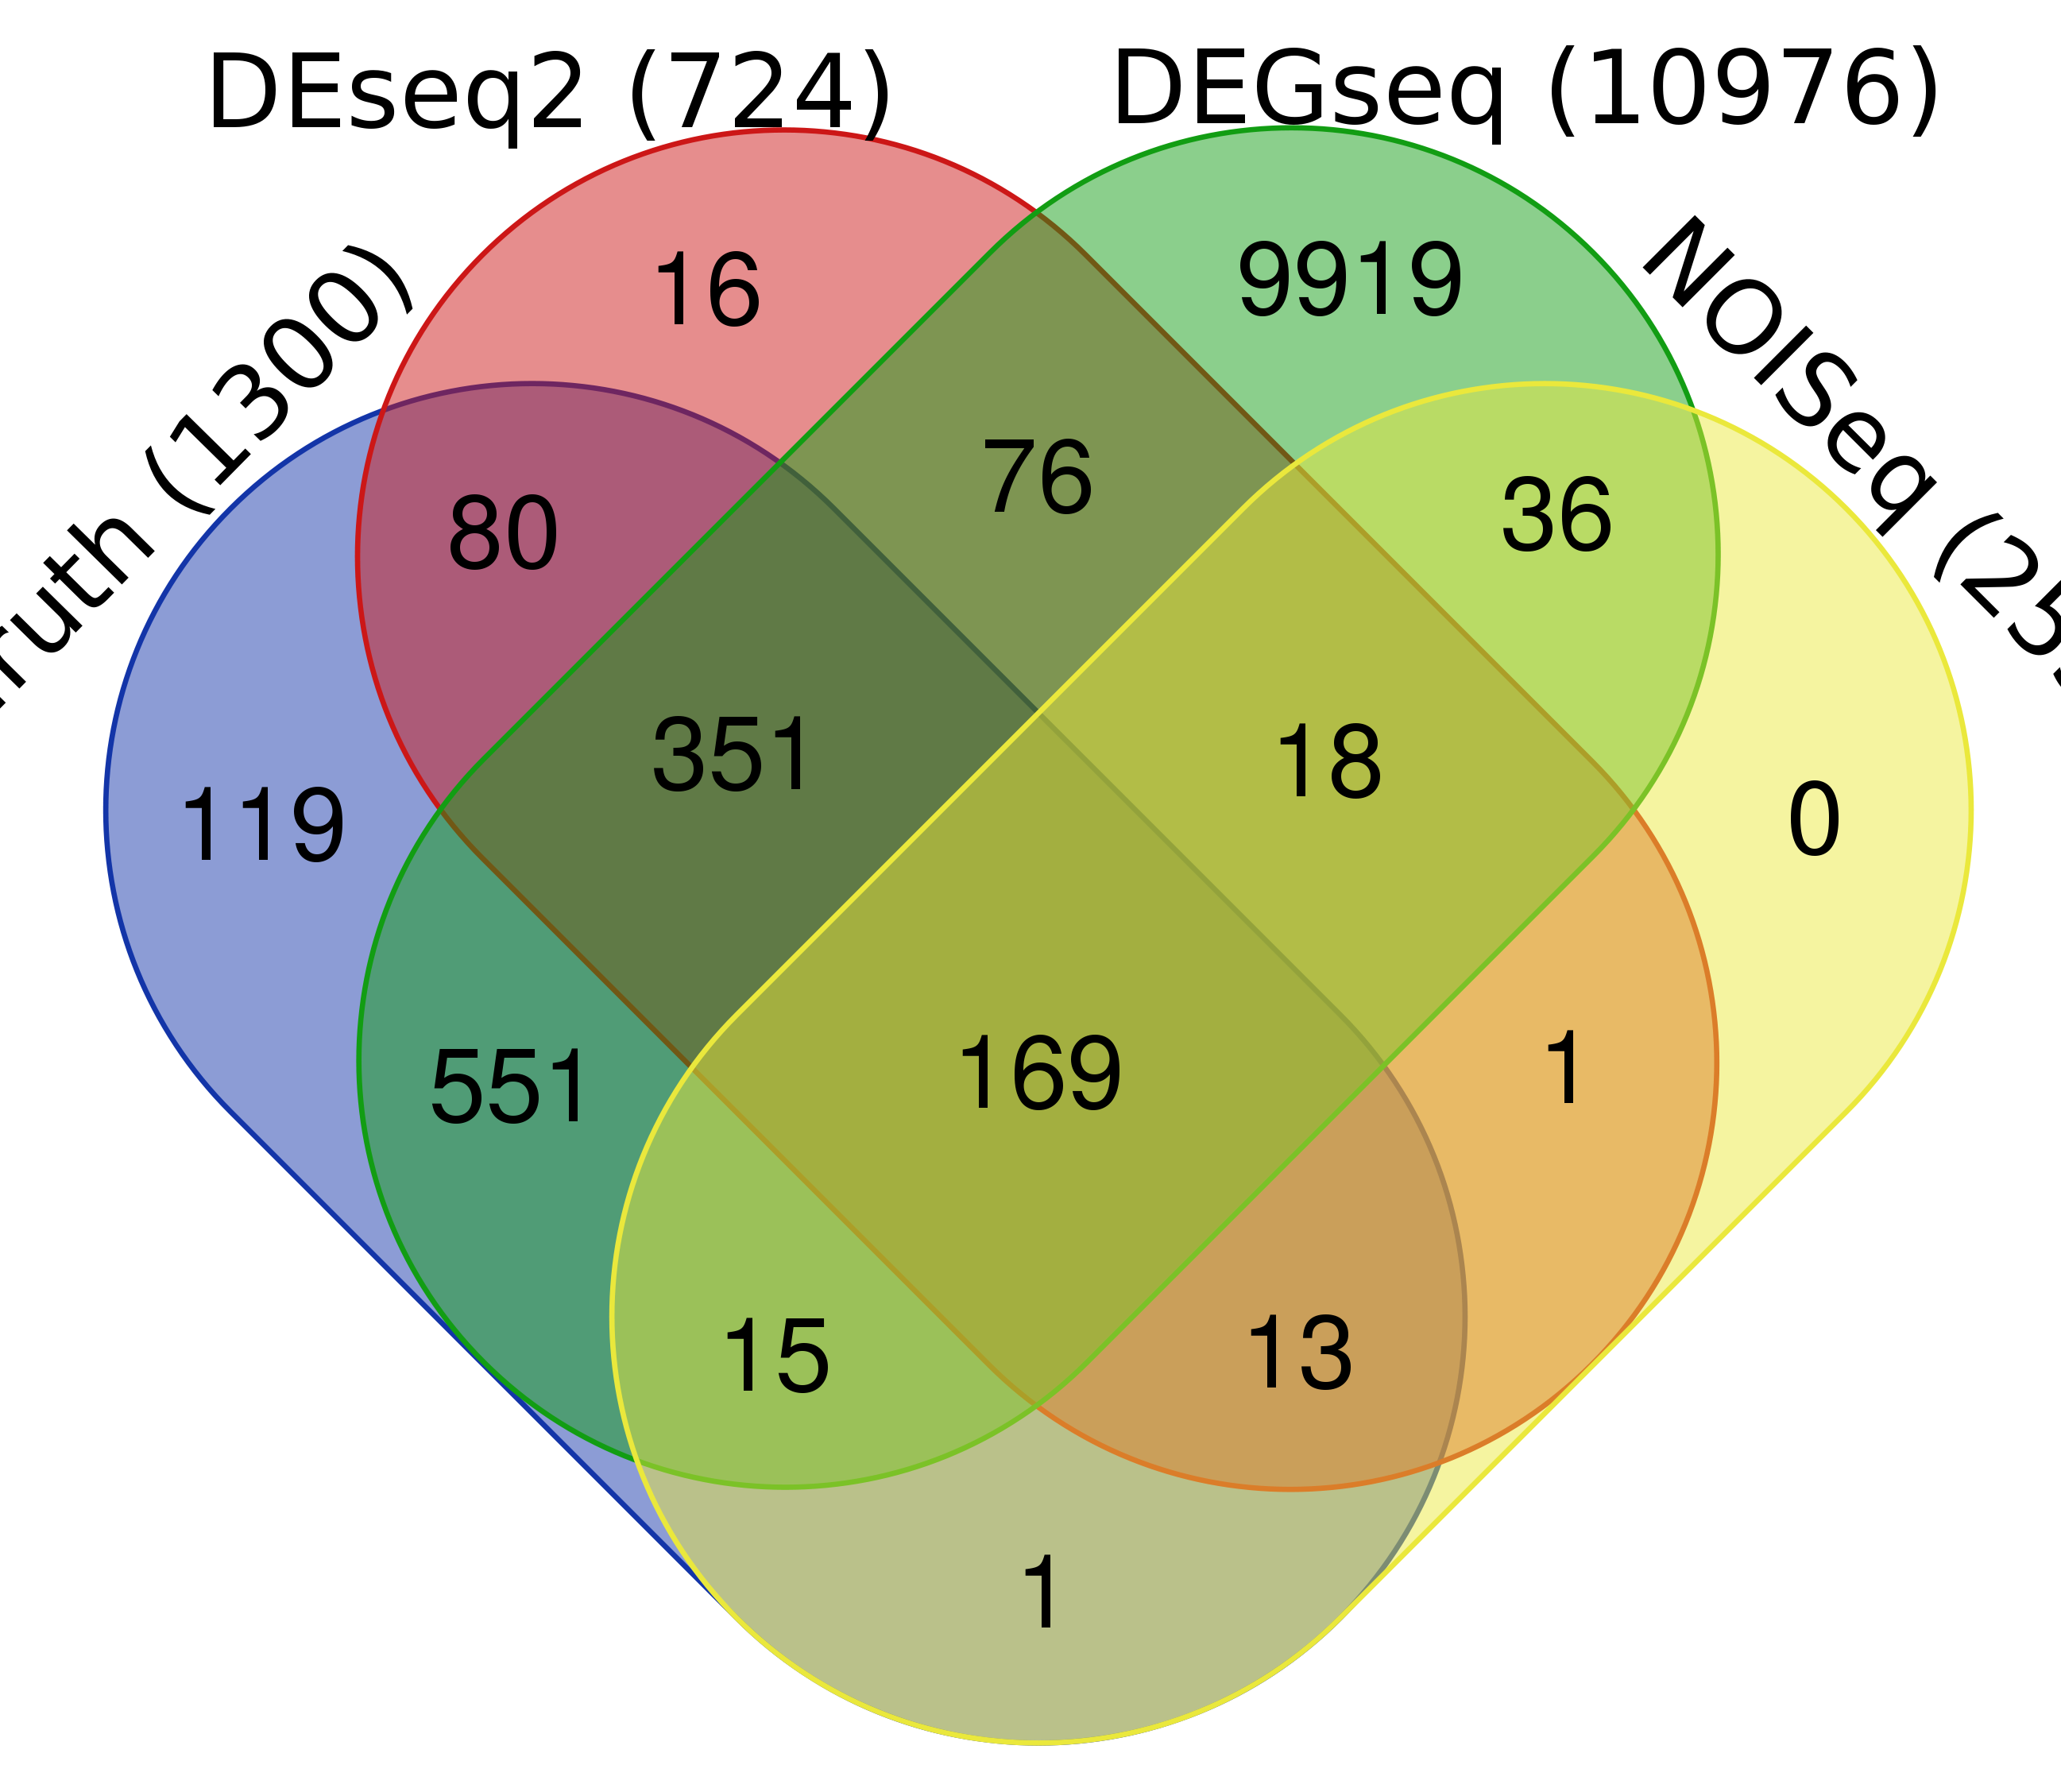
\includegraphics[width=0.33\linewidth]{/Users/abdul-rahmanbukari/Documents/BIOSTATS/Project/D2venn_result}
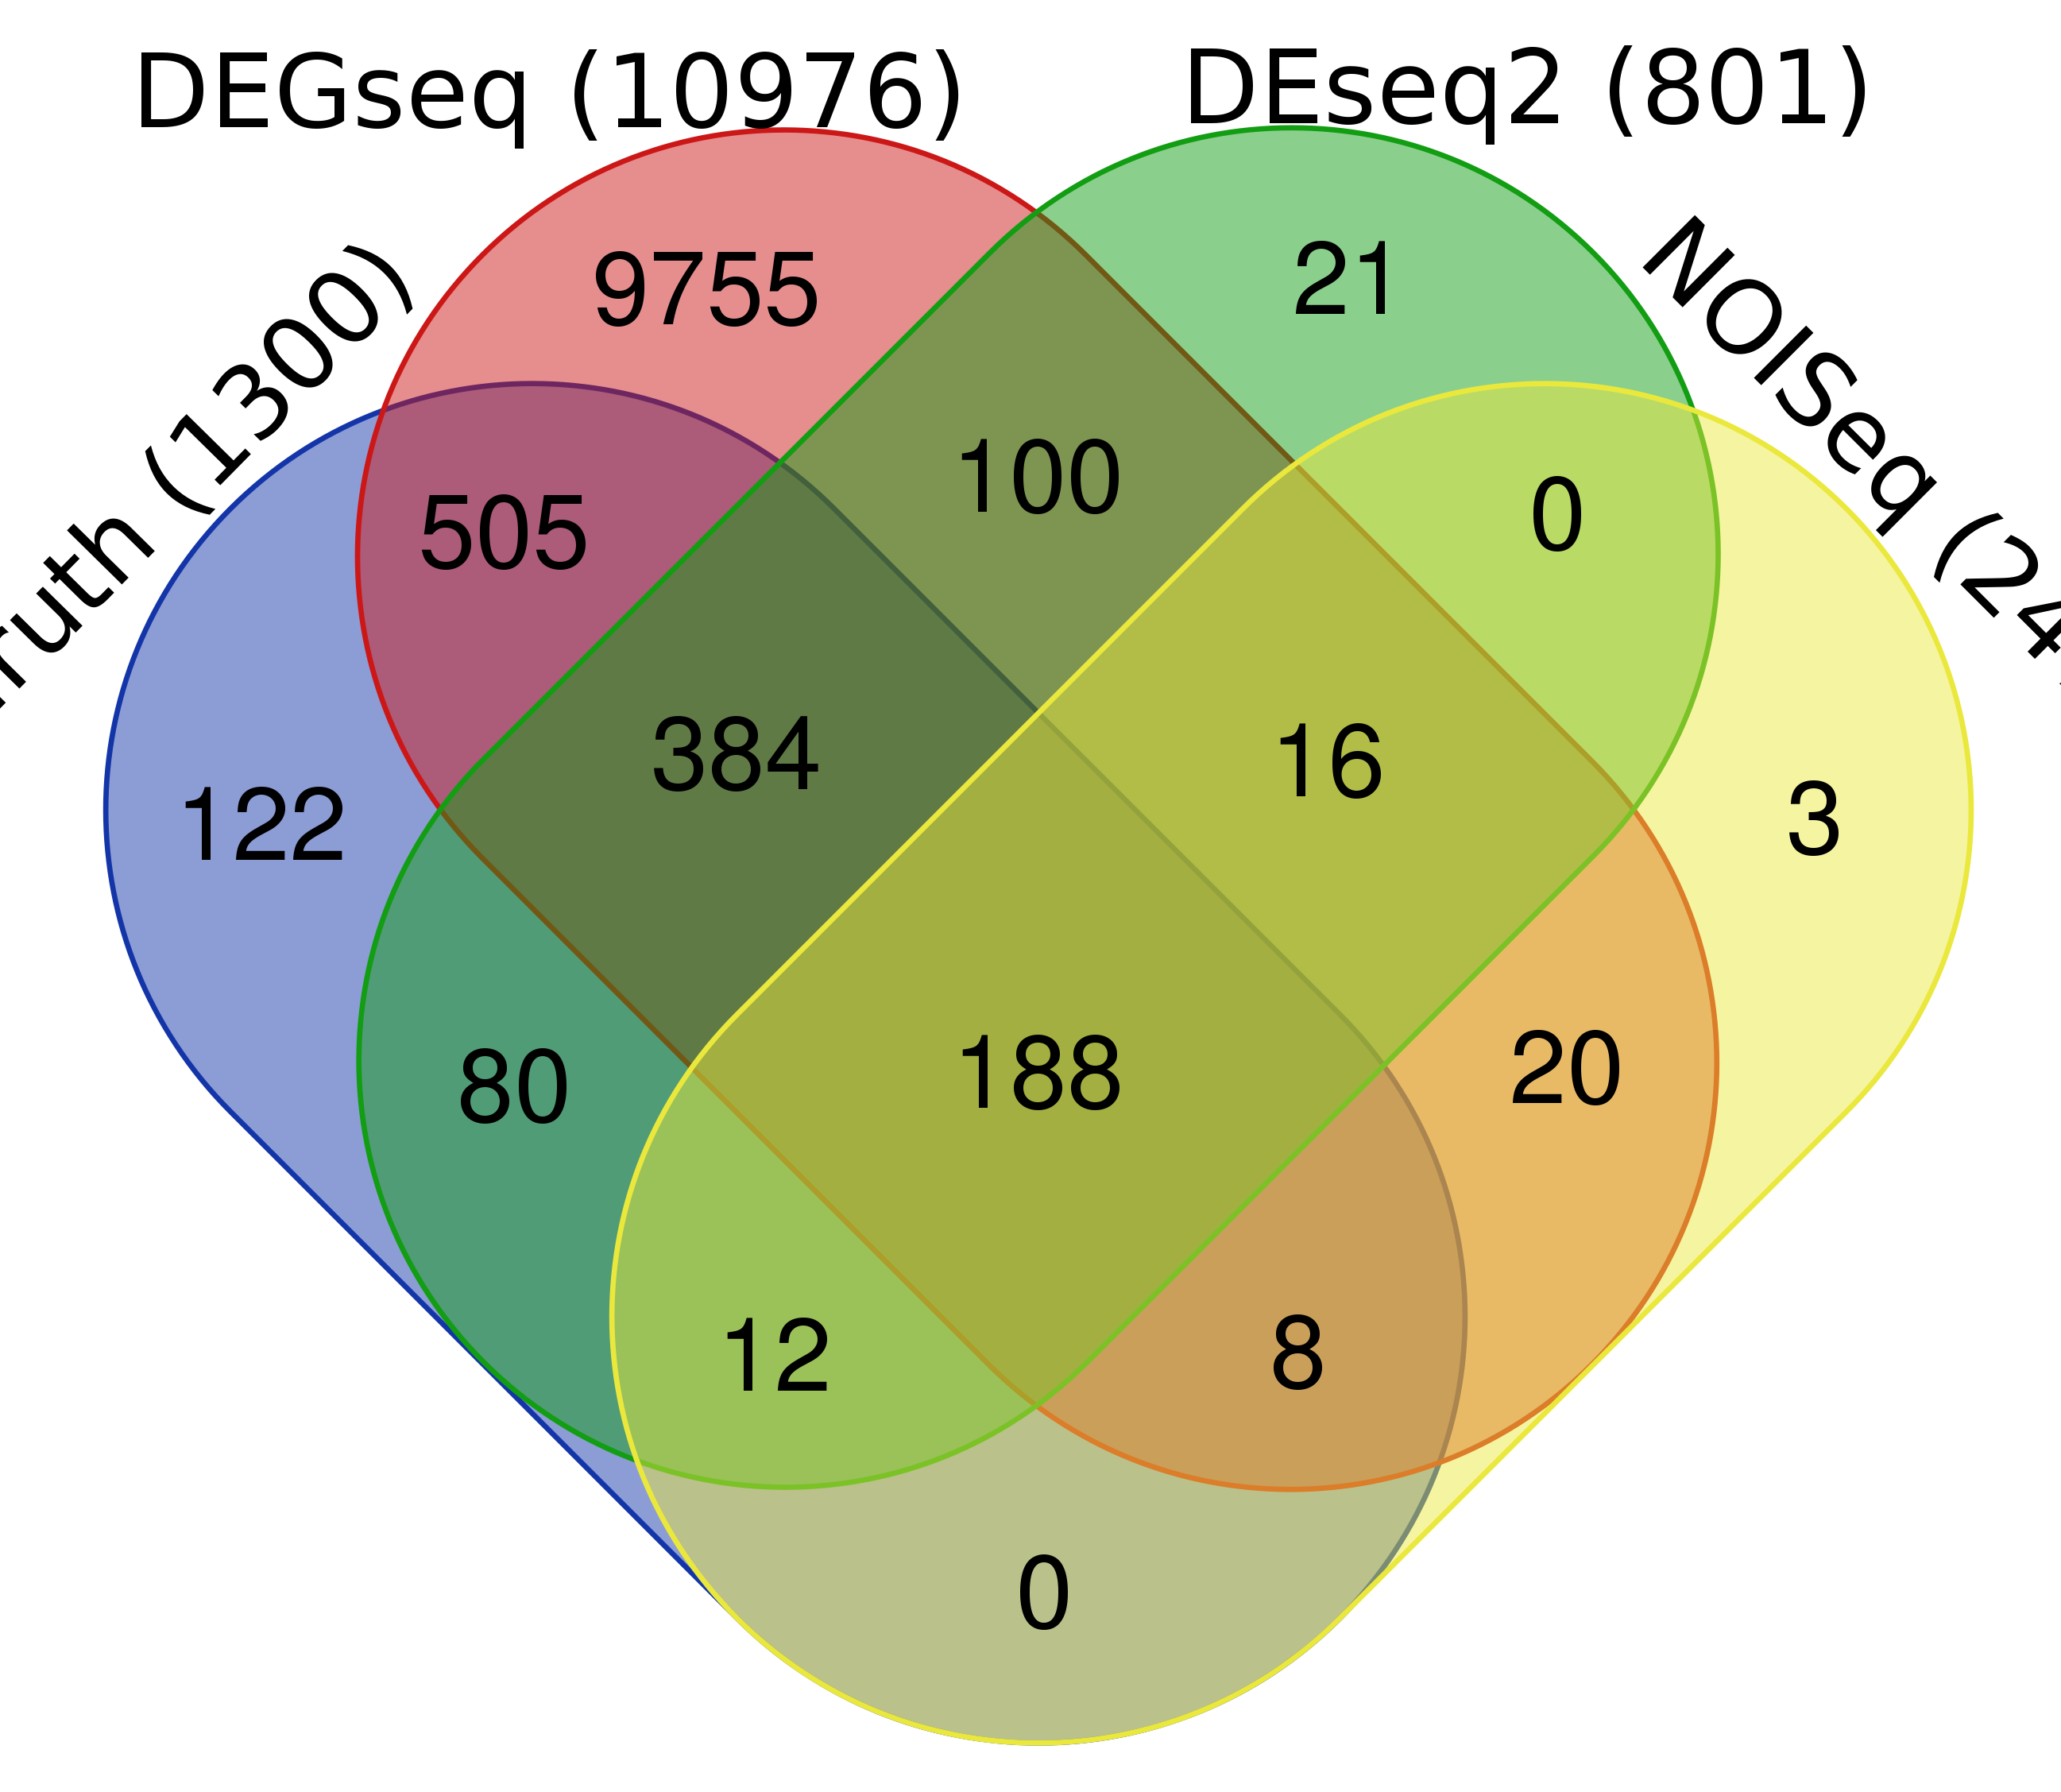
\includegraphics[width=0.33\linewidth]{/Users/abdul-rahmanbukari/Documents/BIOSTATS/Project/D3venn_result}
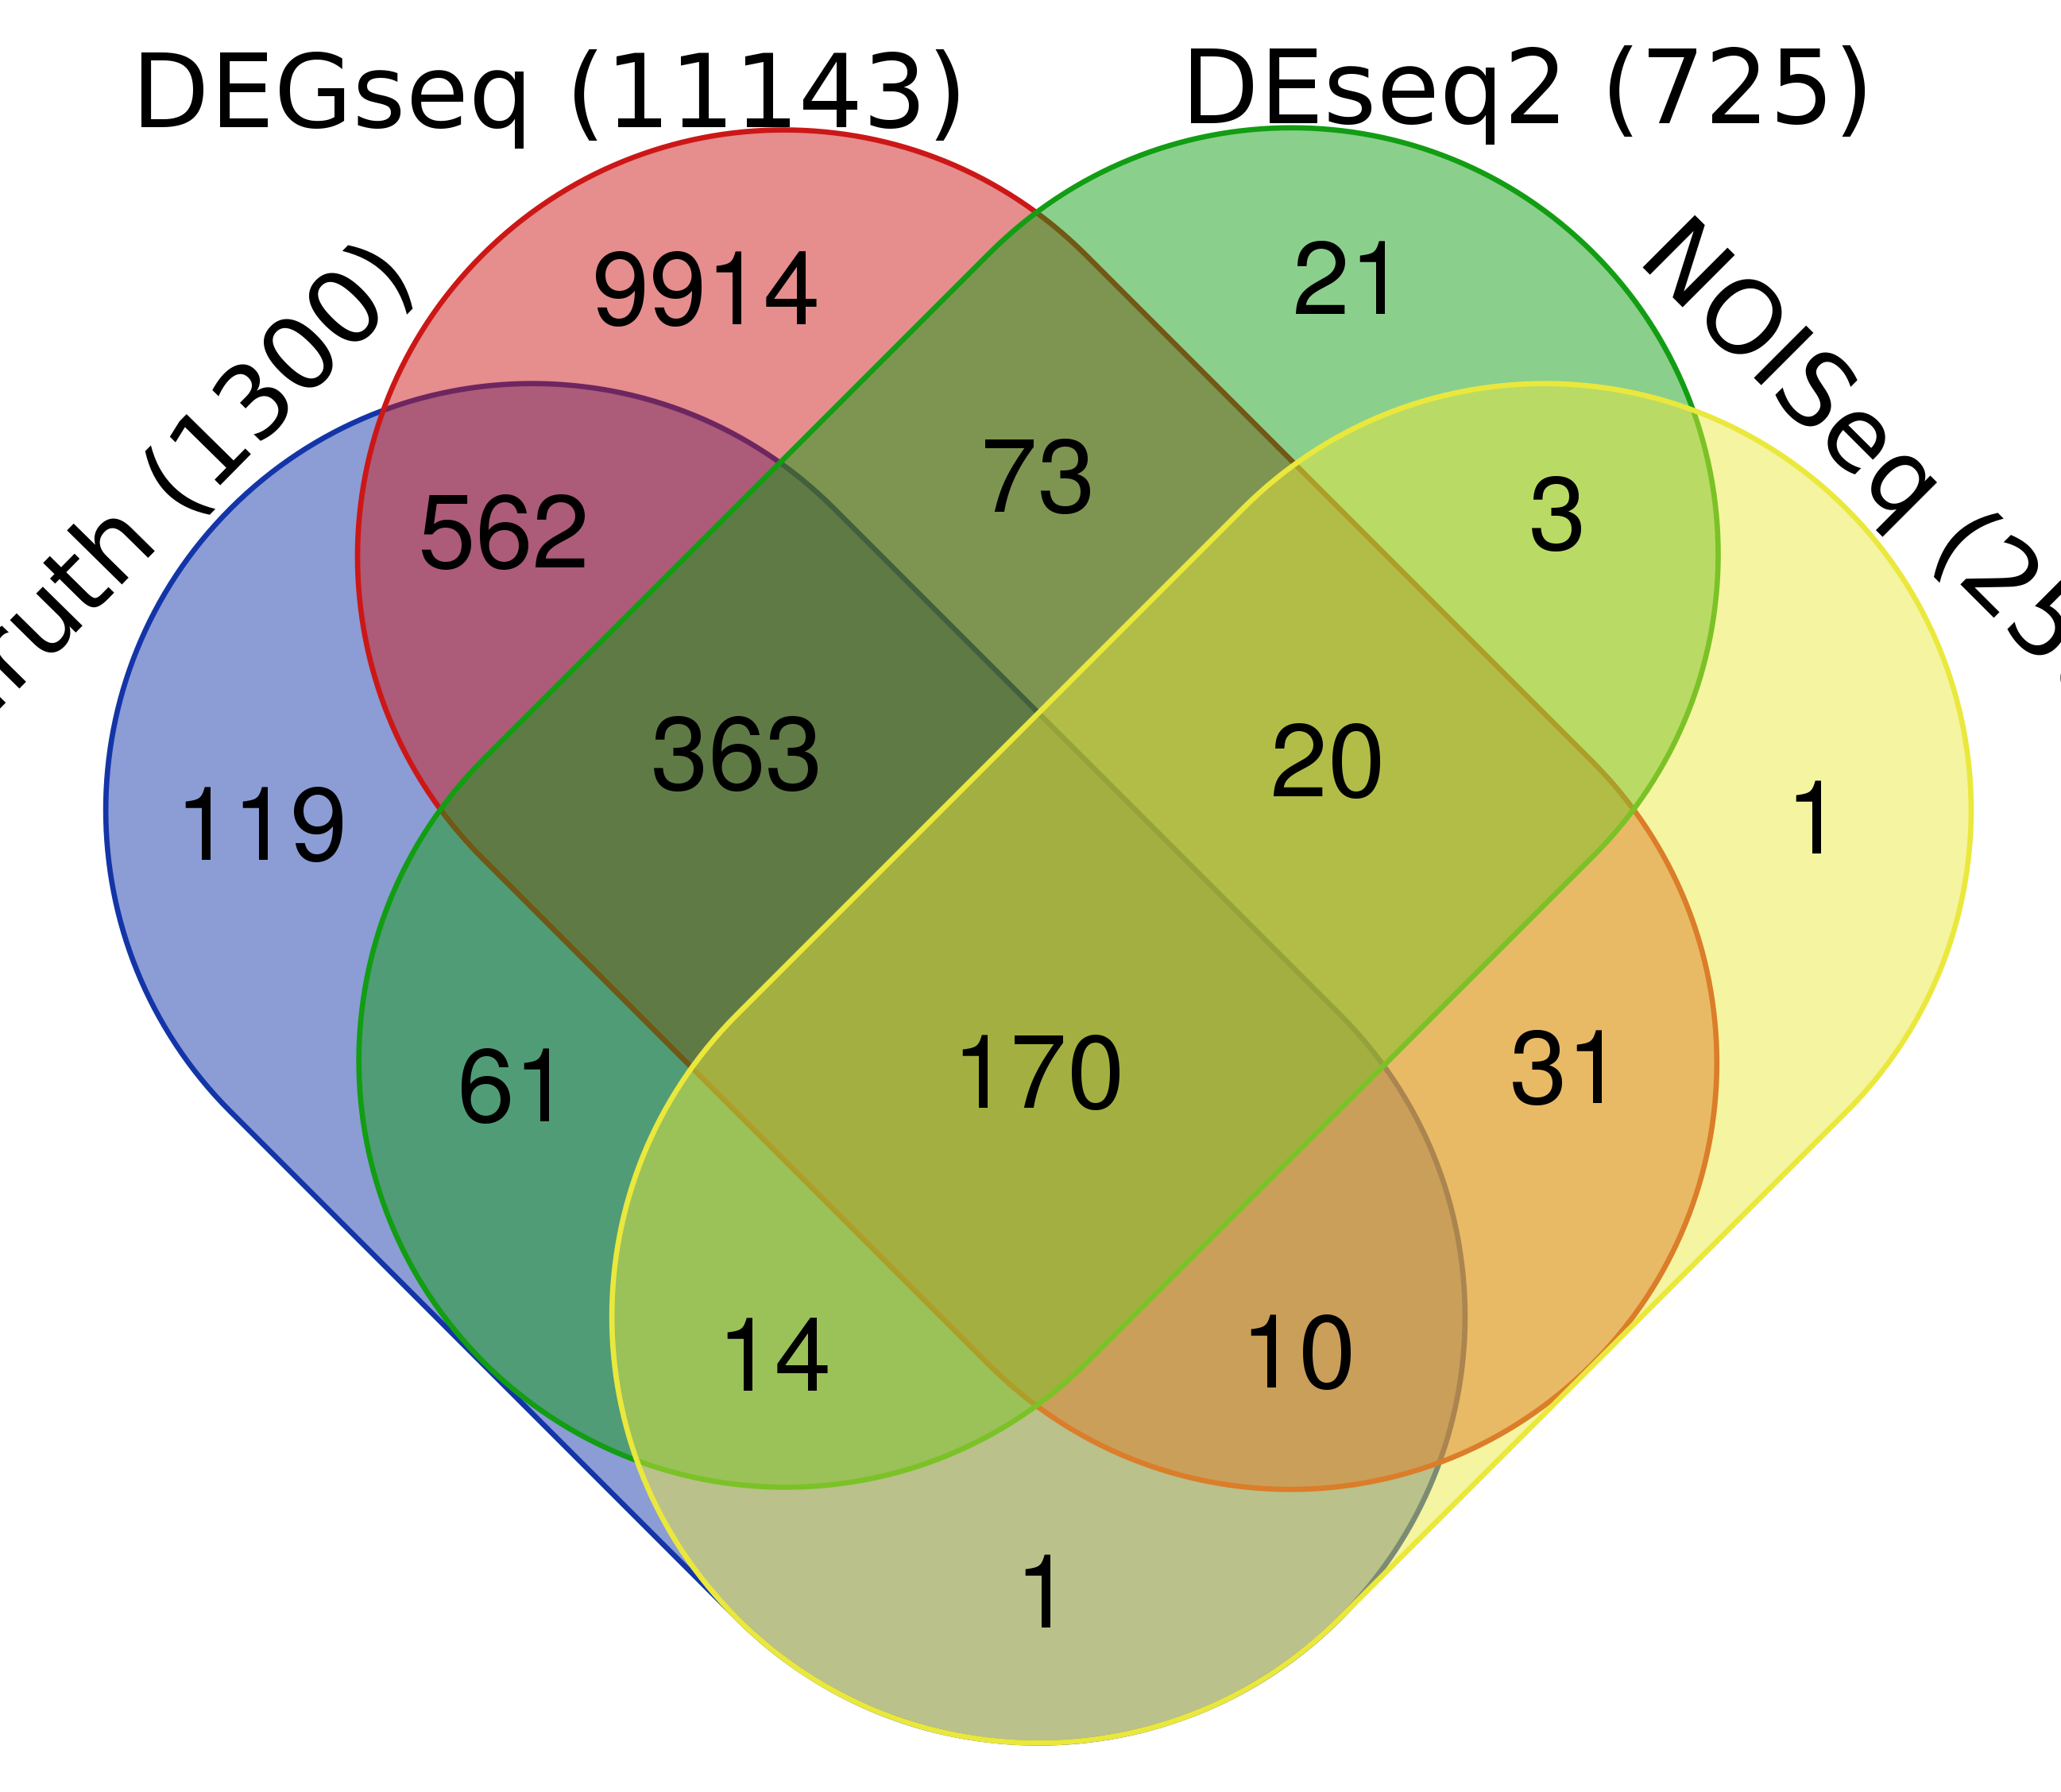
\includegraphics[width=0.33\linewidth]{/Users/abdul-rahmanbukari/Documents/BIOSTATS/Project/D4venn_result}

\begin{Shaded}
\begin{Highlighting}[]
\CommentTok{#Extract the true positives, false negatives and fasle positives to calculate the average prescision, recall and specificity using the venn diagrames}
\NormalTok{Tools =}\StringTok{ }\KeywordTok{rep}\NormalTok{(}\KeywordTok{c}\NormalTok{(}\StringTok{"DESeq2"}\NormalTok{,}\StringTok{"DEGseq"}\NormalTok{,}
              \StringTok{"NOISeq"}\NormalTok{),}\DecValTok{3}\NormalTok{)}


\NormalTok{Precision  =}\StringTok{ }\KeywordTok{c}\NormalTok{(}\FloatTok{0.836550585}\NormalTok{,}
\FloatTok{0.098348461}\NormalTok{,}
\FloatTok{0.790398673}\NormalTok{)}

\NormalTok{Recall =}\StringTok{ }\KeywordTok{c}\NormalTok{(}\FloatTok{0.47691982}\NormalTok{,}
\FloatTok{0.834744478}\NormalTok{,}
\FloatTok{0.147367798}\NormalTok{)}

\NormalTok{F1Score =}\StringTok{ }\KeywordTok{c}\NormalTok{(}\FloatTok{0.612968476}\NormalTok{,}
\FloatTok{0.1763581}\NormalTok{,}
\FloatTok{0.258616348}\NormalTok{)}

\NormalTok{Performace_measures <-}\KeywordTok{c}\NormalTok{(Precision, Recall, F1Score)}
\NormalTok{type <-}\KeywordTok{c}\NormalTok{(}\KeywordTok{rep}\NormalTok{(}\StringTok{"Precision"}\NormalTok{, }\DecValTok{3}\NormalTok{), }\KeywordTok{rep}\NormalTok{(}\StringTok{"Recall"}\NormalTok{, }\DecValTok{3}\NormalTok{),}\KeywordTok{rep}\NormalTok{(}\StringTok{"F1Score"}\NormalTok{, }\DecValTok{3}\NormalTok{))}
\NormalTok{mydata <-}\KeywordTok{data.frame}\NormalTok{(Tools, Performace_measures)}
\NormalTok{sdev <-}\StringTok{ }\KeywordTok{c}\NormalTok{(}\FloatTok{0.019350095}\NormalTok{,}
          \FloatTok{0.001178943}\NormalTok{,}
          \FloatTok{0.006497606}\NormalTok{, }\FloatTok{0.020722494}\NormalTok{,}
          \FloatTok{0.014285714}\NormalTok{,}
          \FloatTok{0.013458174}\NormalTok{, }\FloatTok{0.018337634}\NormalTok{,}
          \FloatTok{0.00219842}\NormalTok{,}
          \FloatTok{0.019011926}\NormalTok{)}

\NormalTok{mydata <-}\KeywordTok{data.frame}\NormalTok{(Tools, Performace_measures,sdev)}
\NormalTok{p <-}\KeywordTok{ggplot}\NormalTok{(mydata, }\KeywordTok{aes}\NormalTok{(Tools, Performace_measures))}
\NormalTok{p }\OperatorTok{+}\KeywordTok{geom_bar}\NormalTok{(}\DataTypeTok{stat =} \StringTok{"identity"}\NormalTok{, }\KeywordTok{aes}\NormalTok{(}\DataTypeTok{fill =}\NormalTok{ type), }\DataTypeTok{position =} \StringTok{"dodge"}\NormalTok{, }\DataTypeTok{width=}\FloatTok{0.7}\NormalTok{)}
\end{Highlighting}
\end{Shaded}

\begin{figure}
\centering
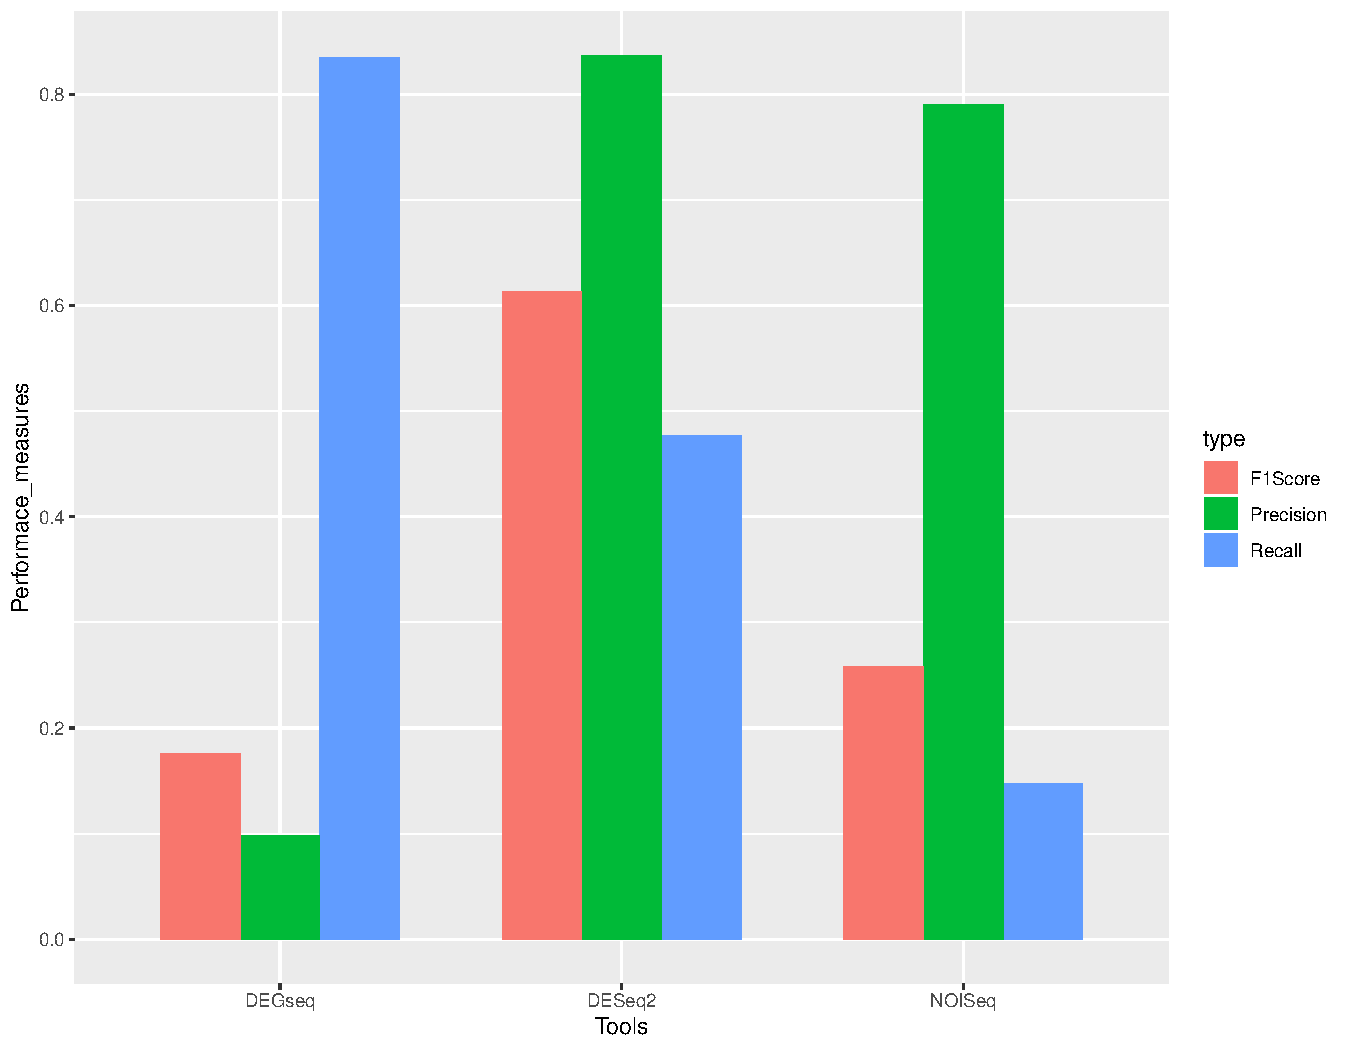
\includegraphics{Untitled_files/figure-latex/Performance measures-1.pdf}
\caption{Performance measures of the tools}
\end{figure}

\hypertarget{discussion}{%
\subsection{Discussion}\label{discussion}}

The differences seen with these three tools may be explained by the
different approaches taken by these tools in the individual steps of the
differential gene expression analyses. We explain the different
approaches employed by these tools in each of the tools. Differential
expression analysis is manily made up of three steps;

\begin{itemize}
\item
  Count Normalization
\item
  Parameter estimation of the statistical model
\end{itemize}

-Test for diffferential expresion

\hypertarget{count-normalization}{%
\subsection{Count Normalization}\label{count-normalization}}

The first step in the DE analysis workflow is count normalization, which
is necessary to make accurate comparisons of gene expression between
samples. Normalization is the process of scaling raw count values to
account for the ``uninteresting'' factors such as sequencing depth, gene
length and RNA composition. Normalization procedures attempt to account
for such differences to facilitate accurate comparisons between sample
groups. While this is essential for differential expression analyses, it
is also necessary for exploratory data analysis, visualization of data,
and whenever you are exploring or comparing counts between or within
samples.

Deseq2 employs the Median of ratios via the \emph{estimateSizeFactors()}
and \emph{sizeFactors()} functions which are automatically incorporated
in the \emph{DESeq} function. In it implementation, counts are are
divided by sample-specific size factors determined by median ratio of
gene counts relative to geometric mean per gene (Anders and Huber
(2010)).

\(\hat{s}_j = median_i \frac{k_{ij} } {(\prod_{v = 1}^{m}K_{iv})^ \frac{1}{m}}\)

Noiseq uses a sligthly different normalization scalling called the
Trimmed mean of M. This calculates a scaling factor between two
experiments by using the weighted average of the log expression ratios
of the subset of genes after excluding genes that exhibit high average
read counts and genes that have large differences in expression
(Robinson and Oshlack (2010)).

\(M_g = log_2 \frac{Y_gk/N_k} {Y_gk^,/N_k^,}\)

\(A_g = \frac{1}{2}log_2 {Y_gk/N_k}*{Y_gk^,/N_k^,}\)

Both approaches are based on strong assumptions that most genes are not
differentially expressed, and that for those differentially expressed
there is an approximately balanced proportion of over- and
under-expression. These two approaches to normalization have been found
to provide comparable performance (Dillies et al. (2013)).

With DEGseq, no normalization approach was selected per strong
recommendation by the developers. In fact specifying a trimmed mean of
count rather degraded the performance with extreamly high false
positives. The lack of a suitable normalization could explain the
degraded results obtained for DEGseq.

\hypertarget{parameter-estimation-of-the-statistical-model-and-test-for-diffferential-expresion}{%
\subsection{Parameter estimation of the statistical model and Test for
diffferential
expresion}\label{parameter-estimation-of-the-statistical-model-and-test-for-diffferential-expresion}}

The goal of a DE analysis is to highlight genes that have changed
significantly in abundance across experimental conditions. In general,
this means taking a table of summarized count data for each library and
performing statistical testing between samples of interest. The models
proposed by these tools is a way to approximate how the data behaves
given a set of parameters (i.e.~size factor, dispersion). This requires
that an assumptions of the distribution of the count data is made and
modelled accordinly to estimate the the parameters of the distribution.

Deseq2 models the normalized count data as a Generalized Linear Model of
a Negative Binomial distribution with a log link. The assumption of a NB
distribution inspired by the percieved overdispersion (variance
\textgreater{} mean) among biological replicates of count data. This
involves estimating the gene-wise dispersions and shrinking these
estimates to generate more accurate estimates of dispersion to model the
counts. The The Wald test is then used as a statistical test for
differenctial expression and the p values are adjusted for multiple
testing using the procedure of Benjamini and Hochberg (Benjamini and
Hochberg (1995)).

\(K_{ij}∼NB(μ_{ij},α_{i})\)

\(μ_{ij}=s_{j}q_{ij}\)

\(log_{2}(q_{ij})=x{j}.β{i}\)

\(Var(K_{ij})=μ_{ij}+α_iμ^2_{ij}\)

DEGseq on the other hand models the counts as a bionomial distribution
which can be approximated by a Poisson distribution (Jiang and Wong
(2009)). This is based on the assumption that RNA sequencing could be
modeled as a random sampling process, in which each read is sampled
independently and uniformly from every possible nucleotide in the
sample. The process is based on MA plots. Given that \(C1\) and \$C\$2
denote the counts of reads mapped to a specific gene obtained from two
replicates groups, with \(Ci ∼ binomial (ni, pi), i = 1, 2..n\) where
\(n_i\) denotes the total number of mapped reads and \(pi\) the
probability of a read coming from that gene; \(M = log2C1- log2C2\), and
\(A = (log_2C_1 + log_2C_2)/2\). Through a series of MA plots, a z-score
can be estimated which is futher used in calculating a p-value during
hypothesis testing via the likloihood ratio test. The binomial
distribution may not be optimal for RNAseq count data as the dispersion
parameter (standard deviation) may not be a good metric.

NOISeq adopts a nonparametric approach for detecting differentially
expressed genes from count data. NOISeq basically creates a null or
noise distribution of count changes by contrasting fold-change
differences (M) and absolute expression differences (D) for all the
genes in samples within the same condition. This reference distribution
is then used to assess whether the (M, D) values computed between two
conditions for a given gene are likely to be part of the noise or
represent a true differential expression

\begin{itemize}
\tightlist
\item
  Pseudocount generation and summarization
\end{itemize}

\(\tilde{y}_{gk}=y_{gk_i}×10^6/m_i\)

\(\tilde{y}_{gk}=∑i_{∈Ck}\tilde{y_{gi}}\)

Calculation of Log ratio (L) and Absolute value difference (D)

\(L = log_2 \frac {\tilde{y}_gC_1}{\tilde{y}_gC_2)}\)

\(D=|\tilde{y}_gC_1−\tilde{y}_gC_2|\)

where C1 and C2 denote group 1 and 2, respectively.

Null hypothesis: L and D values are no different than noise if not DE.
This is tested via the Wilcoxon test.

Probability distribution for random variables \(L*\) and \(D*\) are
estimated as noise

Probability of being differentially expresssed is estimated and a
predifined odds ratio used to decide whether a gene is differentially
expressed between the two conditions or not.

This approach makes NOISeq robust maintaining a high true-positive rate.
However, there is high positive rate (Huang, Niu, and Qin (2015)) at a
low count range leading to what was observed in our study.

\hypertarget{conclusion}{%
\subsection{Conclusion}\label{conclusion}}

Here, it is shown that the approached adopted by various differential
expression analyses tool at each stage of the analysis is crucial.
Reserchers indending to use these tools should have a good idea of the
normalization, distribution and hypothesis testing approach suitable for
their data. This knowledge in addition to the experimental design should
then inform the appropriate analysis packe to employ. This can be
achieved by doing a series of exploratory anaysis to analyze the
distribution of the data.

We have shown that count data from a pairwise experimental design with
replicates following a binomial distribution (as is often seen of
RNA-seq count data)

\hypertarget{references}{%
\subsection*{References}\label{references}}
\addcontentsline{toc}{subsection}{References}

\hypertarget{refs}{}
\leavevmode\hypertarget{ref-anders2010differential}{}%
Anders, Simon, and Wolfgang Huber. 2010. ``Differential Expression
Analysis for Sequence Count Data.'' \emph{Genome Biology} 11 (10).
BioMed Central: R106.

\leavevmode\hypertarget{ref-benjamini1995controlling}{}%
Benjamini, Yoav, and Yosef Hochberg. 1995. ``Controlling the False
Discovery Rate: A Practical and Powerful Approach to Multiple Testing.''
\emph{Journal of the Royal Statistical Society: Series B
(Methodological)} 57 (1). Wiley Online Library: 289--300.

\leavevmode\hypertarget{ref-dillies2013comprehensive}{}%
Dillies, Marie-Agnès, Andrea Rau, Julie Aubert, Christelle
Hennequet-Antier, Marine Jeanmougin, Nicolas Servant, Céline Keime, et
al. 2013. ``A Comprehensive Evaluation of Normalization Methods for
Illumina High-Throughput Rna Sequencing Data Analysis.'' \emph{Briefings
in Bioinformatics} 14 (6). Oxford University Press: 671--83.

\leavevmode\hypertarget{ref-huang2015differential}{}%
Huang, Huei-Chung, Yi Niu, and Li-Xuan Qin. 2015. ``Differential
Expression Analysis for Rna-Seq: An Overview of Statistical Methods and
Computational Software: Supplementary Issue: Sequencing Platform
Modeling and Analysis.'' \emph{Cancer Informatics} 14. SAGE Publications
Sage UK: London, England: CIN--S21631.

\leavevmode\hypertarget{ref-jiang2009statistical}{}%
Jiang, Hui, and Wing Hung Wong. 2009. ``Statistical Inferences for
Isoform Expression in Rna-Seq.'' \emph{Bioinformatics} 25 (8). Oxford
University Press: 1026--32.

\leavevmode\hypertarget{ref-robinson2010scaling}{}%
Robinson, Mark D, and Alicia Oshlack. 2010. ``A Scaling Normalization
Method for Differential Expression Analysis of Rna-Seq Data.''
\emph{Genome Biology} 11 (3). BioMed Central: R25.

\leavevmode\hypertarget{ref-robles2012efficient}{}%
Robles, José A, Sumaira E Qureshi, Stuart J Stephen, Susan R Wilson,
Conrad J Burden, and Jennifer M Taylor. 2012. ``Efficient Experimental
Design and Analysis Strategies for the Detection of Differential
Expression Using Rna-Sequencing.'' \emph{BMC Genomics} 13 (1). BioMed
Central: 484.

\leavevmode\hypertarget{ref-soneson2013comparison}{}%
Soneson, Charlotte, and Mauro Delorenzi. 2013. ``A Comparison of Methods
for Differential Expression Analysis of Rna-Seq Data.'' \emph{BMC
Bioinformatics} 14 (1). BioMed Central: 91.


\end{document}
